%% (Master) Thesis template
% Template version used: v1.4
%
% Largely adapted from Adrian Nievergelt's template for the ADPS
% (lecture notes) project.



%% We use the memoir class because it offers a many easy to use features.
\documentclass[11pt,a4paper,table,hidelinks]{memoir}  % Remove "hidelinks" for red boxes around hyperlinks

%% Packages
%% ========

%% LaTeX Font encoding -- DO NOT CHANGE
\usepackage[OT1]{fontenc}

%% Babel provides support for languages.  'english' uses British
%% English hyphenation and text snippets like "Figure" and
%% "Theorem". Use the option 'ngerman' if your document is in German.
%% Use 'american' for American English.  Note that if you change this,
%% the next LaTeX run may show spurious errors.  Simply run it again.
%% If they persist, remove the .aux file and try again.
\usepackage[english]{babel}

%% Input encoding 'utf8'. In some cases you might need 'utf8x' for
%% extra symbols. Not all editors, especially on Windows, are UTF-8
%% capable, so you may want to use 'latin1' instead.
\usepackage[utf8]{inputenc}

%% This changes default fonts for both text and math mode to use Herman Zapfs
%% excellent Palatino font.  Do not change this.
%\usepackage[sc]{mathpazo}

%% The AMS-LaTeX extensions for mathematical typesetting.  Do not
%% remove.
\usepackage{amsmath,amssymb,amsfonts,mathrsfs}

%% NTheorem is a reimplementation of the AMS Theorem package. This
%% will allow us to typeset theorems like examples, proofs and
%% similar.  Do not remove.
%% NOTE: Must be loaded AFTER amsmath, or the \qed placement will
%% break
\usepackage[amsmath,thmmarks]{ntheorem}

%% LaTeX' own graphics handling
\usepackage{graphicx}

%% We unfortunately need this for the Rules chapter.  Remove it
%% afterwards; or at least NEVER use its underlining features.
\usepackage{soul}

%% This allows you to add .pdf files. It is used to add the
%% declaration of originality.
\usepackage{pdfpages}

\newenvironment{conditions}
  {\par\vspace{\abovedisplayskip}\noindent\begin{tabular}{>{$}l<{$} @{${}={}$} l}}
  {\end{tabular}\par\vspace{\belowdisplayskip}}

%% Some more packages that you may want to use.  Have a look at the
%% file, and consult the package docs for each.
%% See the TeXed file for more explanations

%% [OPT] Multi-rowed cells in tabulars
%\usepackage{multirow}

%% [REC] Intelligent cross reference package. This allows for nice
%% combined references that include the reference and a hint to where
%% to look for it.
\usepackage{varioref}

%% [OPT] Easily changeable quotes with \enquote{Text}
%\usepackage[german=swiss]{csquotes}

%% [REC] Format dates and time depending on locale
\let\ordinal\relax %% prevent warning
\usepackage{datetime}

%% [OPT] Provides a \cancel{} command to stroke through mathematics.
%\usepackage{cancel}

%% [NEED] This allows for additional typesetting tools in mathmode.
%% See its excellent documentation.
\usepackage{mathtools}

%% [NEED] Conditional commands
\usepackage{ifthen}

%% [OPT] Manual large braces or other delimiters.
%\usepackage{bigdelim, bigstrut}

%% [REC] Alternate vector arrows. Use the command \vv{} to get scaled
%% vector arrows.
\usepackage[h]{esvect}

%% [NEED] Some extensions to tabulars and array environments.
\usepackage{array}

%% [OPT] Postscript support via pstricks graphics package. Very
%% diverse applications.
%\usepackage{pstricks,pst-all}

%% [?] This seems to allow us to define some additional counters.
%\usepackage{etex}

%% [ADV] XY-Pic to typeset some matrix-style graphics
%\usepackage[all]{xy}

%% [OPT] This is needed to generate an index at the end of the
%% document.
%\usepackage{makeidx}

%% [OPT] Fancy package for source code listings.  The template text
%% needs it for some LaTeX snippets; remove/adapt the \lstset when you
%% remove the template content.
\usepackage{listings}
% \lstset{language=TeX,basicstyle={\normalfont\ttfamily}}

%% [REC] Fancy character protrusion.  Must be loaded after all fonts.
%\usepackage[activate]{pdfcprot}

%% [REC] Nicer tables.  Read the excellent documentation.
\usepackage{booktabs}

%% [OPT] Package for adding TODOs.
\usepackage{todonotes}

%% [OPT] Package to define and use acronyms
\usepackage[nolist,nohyperlinks,smaller]{acronym}
 

%% Our layout configuration.  DO NOT CHANGE.
%% Memoir layout setup

%% NOTE: You are strongly advised not to change any of them unless you
%% know what you are doing.  These settings strongly interact in the
%% final look of the document.

% Dependencies
%\usepackage{ETHlogo}

% use helvetica as default font:
\usepackage[scaled]{helvet}
%\renewcommand\familydefault{\sfdefault} 

% Turn extra space before chapter headings off.
\setlength{\beforechapskip}{0pt}

\nonzeroparskip
\parindent=0pt
\defaultlists

% Chapter style redefinition
\makeatletter

\makepagestyle{headerWPageNr}% Create headerWPageNr style
\if@twoside
  \copypagestyle{headerWPageNr}{Ruled}
  \copypagestyle{chapter}{Ruled}
\else
  \copypagestyle{headerWPageNr}{ruled}
  \copypagestyle{chapter}{ruled}
\fi
% chapter pages have no header and center page number in footer:
\makeoddhead{chapter}{}{}{}
\makeevenhead{chapter}{}{}{}
\makeoddfoot{chapter}{}{\thepage}{}
\makeevenfoot{chapter}{}{\thepage}{}
\makeheadrule{chapter}{\textwidth}{0pt}

% all other pages have page number and chapter or section name in header without footer:
\makeoddhead{headerWPageNr}{\rightmark}{}{\thepage}
\makeevenhead{headerWPageNr}{\thepage}{}{\leftmark}
\makeoddfoot{headerWPageNr}{}{}{}
\makeevenfoot{headerWPageNr}{}{}{}
\pagestyle{headerWPageNr}% Set page style to headerWPageNr


\makechapterstyle{bianchimod}{%
  \copypagestyle{abstract}{empty}
  \chapterstyle{default}
  \renewcommand*{\chapnamefont}{\normalfont\Large\sffamily}
  \renewcommand*{\chapnumfont}{\normalfont\Large\sffamily}
  \renewcommand*{\printchaptername}{%
    \chapnamefont\centering\@chapapp}
  \renewcommand*{\printchapternum}{\chapnumfont {\thechapter}}
  \renewcommand*{\chaptitlefont}{\normalfont\huge\sffamily}
  \renewcommand*{\printchaptertitle}[1]{%
    \hrule\vskip\onelineskip \centering \chaptitlefont\textbf{\vphantom{gyM}##1}\par}
  \renewcommand*{\afterchaptertitle}{\vskip\onelineskip \hrule\vskip
    \afterchapskip}
  \renewcommand*{\printchapternonum}{%
    \vphantom{\chapnumfont {9}}\afterchapternum}}
  
\makechapterstyle{bianchimod2}{%
  \renewenvironment{abstract}{\chapter*{\abstractname}}{}
  \chapterstyle{default}
  \definecolor{ChapGrey}{rgb}{0.6,0.6,0.6}
  \newcommand{\LargeFont}{% Needs a ’stretchable’ font
  	\usefont{\encodingdefault}{\sfdefault}{b}{n}%
    \fontsize{100}{0}\selectfont\color{ChapGrey}}
  \renewcommand*{\chapnumfont}{\LargeFont}
  \renewcommand*{\printchaptername}{\raggedleft}
  \renewcommand*{\printchapternum}{\chapnumfont {\thechapter}}
  \renewcommand*{\chaptitlefont}{\normalfont\Huge\sffamily\color{black}}
  \renewcommand*{\printchaptertitle}[1]{%
    \raggedleft \chaptitlefont\textbf{\vphantom{gyM}##1}\par}}

% Use the newly defined style
\chapterstyle{bianchimod2}

\setsecheadstyle{\Large\bfseries\sffamily}
\setsubsecheadstyle{\large\bfseries\sffamily}
\setsubsubsecheadstyle{\bfseries\sffamily}
\setparaheadstyle{\normalsize\bfseries\sffamily}
\setsubparaheadstyle{\normalsize\itshape\sffamily}
\setsubparaindent{0pt}

% Set captions to a more separated style for clearness
\captionnamefont{\sffamily\bfseries\footnotesize}
\captiontitlefont{\sffamily\footnotesize}
\setlength{\intextsep}{16pt}
\setlength{\belowcaptionskip}{1pt}

% Set section and TOC numbering depth to subsection
\setsecnumdepth{subsection}
\settocdepth{subsection}

% definitions for titlepage
\def\@advisor{}
\newcommand{\advisor}[1]{\def\@advisor{#1}}
\def\@supervisor{}
\newcommand{\supervisor}[1]{\def\@supervisor{#1}}
\def\@group{}
\newcommand{\group}[1]{\def\@group{#1}}
\def\@institute{}
\newcommand{\institute}[1]{\def\@institute{#1}}
\def\@department{}
\newcommand{\department}[1]{\def\@department{#1}}
\def\@school{}
\newcommand{\school}[1]{\def\@school{#1}}
\def\@thesistype{}
\newcommand{\thesistype}[1]{\def\@thesistype{#1}}
\def\@email{}
\newcommand{\email}[1]{\def\@email{#1}}

%% Title page adjustments
% the following definition (either 0 or 1) controls the title page's layout:
\def\centeredtitlepage{0}
\if\centeredtitlepage1
	% default title page from cadmo template
	\newcommand{\maketitlepage}{
		\begin{titlingpage}
  			\calccentering{\unitlength}
  			\begin{adjustwidth*}{\unitlength-24pt}{-\unitlength-24pt}
    		\maketitle
  			\end{adjustwidth*}
		\end{titlingpage}
	}
	\pretitle{\vspace{0pt plus 0.7fill}\begin{center}\HUGE\sffamily\bfseries}
	\posttitle{\end{center}\par}
	\preauthor{\par\begin{center}\let\and\\\Large\sffamily}
	\postauthor{\end{center}}
	\predate{\par\begin{center}\Large\sffamily}
	\postdate{\end{center}}

	\renewcommand{\maketitlehooka}{\noindent\ETHlogo[2in]}

	\renewcommand{\maketitlehookb}{\vspace{1in}%
  		\par\begin{center}\Large\sffamily\@thesistype\end{center}}

	\renewcommand{\maketitlehookd}{%
  		\vfill\par
  			\begin{flushright}
    			\sffamily
    			Advisors: \@supervisor, \@advisor\par
    			\@department, \@school
  			\end{flushright}
	}

\else
	% alternative title page (right-aligned)
	\newcommand{\maketitlepage}{
		\begin{titlingpage}
			\titlestyleright
		\end{titlingpage}
	}
	\newcommand*\titlestyleright{
		\thispagestyle{empty}
		\begin{minipage}[c]{0.35\linewidth}
			\vspace{0pt}
			\hfuzz=5.0pt
			
\includegraphics[width=0.9\linewidth]{images/ost_logo_de_rgb-eps-converted-to}
		\end{minipage}
		%
		\begin{minipage}[c]{0.4\linewidth}
			\vspace{0pt}
			\-\
		\end{minipage}
		%
		\begin{minipage}[c]{0.25\linewidth}
			\vspace{0pt}
			\hfuzz=5.0pt
			    \hspace*{-1cm} 
			        
\includegraphics[width=1.3\linewidth]{images/onway_logo}
		\end{minipage}
		\vspace{2cm}
		\sffamily
		\vspace*{\stretch{6}}
		\begin{flushright}
		{\Huge\sffamily\bfseries\@title\par}
		\par\noindent\rule[-1ex]{\linewidth}{2pt}\par
		\vspace{0.5cm}
		\emph{\huge\sffamily\@thesistype}
		\vspace{2cm}\par
		{\LARGE\sffamily\bfseries Florian Baumgartner}\par
		{\sffamily\ \href{mailto:florian.baumgartner@ost.ch}{florian.baumgartner@ost.ch}}\par
		\vspace{0.5cm}
		{\LARGE\sffamily\bfseries Luca Jost}\par
		{\sffamily\ \href{mailto:luca.jost@ost.ch}{luca.jost@ost.ch}}\par
		\vspace{1cm}
    	{\large\textbf{Advisor}\par
    		\@advisor\par}
    	\vspace{0.5cm}
    	{\large\textbf{Examiner}\par
    		\@supervisor\par}
    	\vspace{1cm}
    	{\@institute\par
        	\@school\par}
    	\vspace{1cm}
    	{\normalsize\@date\par}
		\end{flushright}
		\vspace{\stretch{1}}
		\noindent
		\pagebreak 
    	\sffamily
    	\thispagestyle{empty} 
	}
\fi

%Change margins
\setlrmarginsandblock{3.5cm}{3cm}{*}
\setulmarginsandblock{3cm}{*}{1}
\checkandfixthelayout

\setlength{\droptitle}{-48pt}

\makeatother

% This defines how theorems should look. Best leave as is.
\theoremstyle{plain}
\setlength\theorempostskipamount{0pt}

%%% Local Variables:
%%% mode: latex
%%% TeX-master: "thesis"
%%% End:


%% Theorem environments.  You will have to adapt this for a German
%% thesis.
%% Theorem-like environments

%% This can be changed according to language. You can comment out the ones you
%% don't need.

\numberwithin{equation}{chapter}

%% German theorems
%\newtheorem{satz}{Satz}[chapter]
%\newtheorem{beispiel}[satz]{Beispiel}
%\newtheorem{bemerkung}[satz]{Bemerkung}
%\newtheorem{korrolar}[satz]{Korrolar}
%\newtheorem{definition}[satz]{Definition}
%\newtheorem{lemma}[satz]{Lemma}
%\newtheorem{proposition}[satz]{Proposition}

%% English variants
\newtheorem{theorem}{Theorem}[chapter]
\newtheorem{example}[theorem]{Example}
\newtheorem{remark}[theorem]{Remark}
\newtheorem{corollary}[theorem]{Corollary}
\newtheorem{definition}[theorem]{Definition}
\newtheorem{lemma}[theorem]{Lemma}
\newtheorem{proposition}[theorem]{Proposition}

%% Proof environment with a small square as a "qed" symbol
\theoremstyle{nonumberplain}
\theorembodyfont{\normalfont}
\theoremsymbol{\ensuremath{\square}}
\newtheorem{proof}{Proof}
%\newtheorem{beweis}{Beweis}


%% Helpful macros.
%% Custom commands
%% ===============

%% Special characters for number sets, e.g. real or complex numbers.
\newcommand{\C}{\mathbb{C}}
\newcommand{\K}{\mathbb{K}}
\newcommand{\N}{\mathbb{N}}
\newcommand{\Q}{\mathbb{Q}}
\newcommand{\R}{\mathbb{R}}
\newcommand{\Z}{\mathbb{Z}}
\newcommand{\X}{\mathbb{X}}

%% Fixed/scaling delimiter examples (see mathtools documentation)
\DeclarePairedDelimiter\abs{\lvert}{\rvert}
\DeclarePairedDelimiter\norm{\lVert}{\rVert}

%% Use the alternative epsilon per default and define the old one as \oldepsilon
\let\oldepsilon\epsilon
\renewcommand{\epsilon}{\ensuremath\varepsilon}

%% Also set the alternate phi as default.
\let\oldphi\phi
\renewcommand{\phi}{\ensuremath{\varphi}}


%% This allow the usage of dashed and dotted lines in tables
\usepackage{arydshln}
\usepackage{hhline}
\usepackage{mathrsfs}
\usepackage{lscape}
\usepackage{siunitx}
\usepackage{caption}
%\usepackage{subcaption}  % Removed this because of subfig
\usepackage{subfig}
\usepackage{textcomp}

\DeclareCaptionFont{fcaption}{\footnotesize}
%\captionsetup{labelfont={sf, bf}, textfont=sf, font=fcaption}
%\captionsetup[sub]{font=fcaption,labelfont={sf}}

%% Make document internal hyperlinks wherever possible. (TOC, references)
%% This MUST be loaded after varioref, which is loaded in 'extrapackages'
%% above.  We just load it last to be safe.
\usepackage[linkcolor=black,colorlinks=false,citecolor=black,filecolor=black]{hyperref}
\usepackage[capitalize, noabbrev]{cleveref}

%\usepackage[showframe]{geometry}% http://ctan.org/pkg/geometry
%\usepackage{lipsum}% http://ctan.org/pkg/lipsum
%\usepackage{graphicx}% http://ctan.org/pkg/graphicx

\usepackage{setspace}
\usepackage{parskip}
\usepackage{wrapfig}
\usepackage{verbatimbox}
\usepackage{bold-extra}
\usepackage{graphbox}
\usepackage{setspace}
\usepackage{framed}
\usepackage{bm}

\NewDocumentCommand{\codeword}{v}{%
\texttt{\textcolor{black}{#1}}%
}
\lstset{language=C,keywordstyle={\bfseries \color{blue}}}

%% Suppress warnings, kind of hack..
\usepackage{silence}
\WarningFilter{glossaries}{Overriding \printglossary}
\WarningFilter{glossaries}{Overriding `theglossary'}
%% Important: Must be last import package, otherwise hyperlinks do not work?!
\usepackage[acronym]{glossaries}

%% Document information
%% ====================

\title{Audio-Beamformer}
\author{}
\email{}
\thesistype{Bachelor's Thesis}
\advisor{Hannes Badertscher}
\supervisor{Gabriel Sidler}
\group{}
\institute{Interdisciplinary Center for Artificial Intelligence}
\department{Department of Computer Science}
\school{Eastern Switzerland University of Applied Sciences}
\date{June 2022}

\makeglossaries
\pagenumbering{Roman}
\apptocmd{\sloppy}{\hbadness 4000\relax}{}{}  %% Suppress Underfull \vbox warning for bibliography
\begin{document}
\frontmatter

%% Title page is autogenerated from document information above.  DO
%% NOT CHANGE.
\hfuzz=6.0pt \maketitlepage

%% The abstract of your thesis.  Edit the file as needed.
\begin{abstract}
Naturally, sound waves propagate in an omnidirectional pattern. However, in some cases, a directional pattern would be preferred. In comparison to light or electromagnetic waves, it turns out to be a very difficult task to focus audio waves in a specific direction. The underlying reason for this behavior comes from the physical long wavelength of the
audible spectrum. \\
This bachelor's thesis concentrates on how to overcome this effect by using higher frequencies in the ultrasonic spectrum and therefore be able to create a highly directional audio beam. In addition, beam-steering methods are applied to change the direction and focus point by software.

In order to achieve a directional sound beam, a linear phased array has been developed, consisting of 19 rows of 8 ultrasonic transducers each. For this, a single PCB, consisting of over 1300 components was specially designed. Two FPGAs modulate the baseband audio signal onto a 40 kHz ultrasonic carrier. First-order Sigma-Delta-Modulators perform the analog conversation in combination with a Class-D amplifier output stage. In addition, each channel can be delayed and attenuated individually. A Raspberry Pi Compute Module 4 is used to apply real-time digital signal processing techniques to further improve the audio quality. Advanced face-detection algorithms are used to locate a target and therefore be able to direct the sound in its direction. As input sources, Bluetooth$^{\circledR}$ and AirPlay$^{\circledR}$ streaming are supported, as well as other input devices, such as USB-Microphones.

The directivity, beam-steering capability, and overall audio quality have been determined in a comprehensive human expertise test. The Audio-Beamformer performs well in all categories and satisfies the project's goals. Especially the range of up to 50 meters is awe-inspiring. \\
The Audio-Beamformer could lead to a real alternative to conventional loudspeakers with some further improvements.
\end{abstract}

\begin{acknowledgement}
We take this opportunity to express gratitude to all of the people that supported us in this bachelor's thesis.

Especially to Hannes Badertscher for the supervision, Dr. Guido Schuster for his theoretical explanations in the field of digital signal processing, Dr. Hans-Dieter Lang for his comprehensive support in designing high-speed electronics, Dorian Amiet for answering questions about the FPGA implementation, Luca Jost for developing the face-tracking algorithm, Caspar Naef for his endurance, Anne Marie O'Neill for the proofreading and all participants of the human expertise test.

We also thank Elvis for the unceasing encouragement and support throughout the entire project.
\end{acknowledgement}
%% reset acronym usage:

%% TOC with the proper setup, do not change.
\cleartorecto
{
    \linespread{1.03}\selectfont{}
    \tableofcontents*       % This asterisk is important to prevent listing "Contents" in the table of contents
}
\mainmatter
\renewcommand{\thefigure}{\thechapter.\arabic{figure}}

\newglossaryentry{esp32}
{
        name=ESP32,
        description={Is a series of low-cost, low-power \acrlong{soc} microcontrollers with integrated Wi-Fi}
}

\newglossaryentry{canopen}
{
        name=CANOpen,
        description={Is a communication protocol and device profile specification for embedded systems used in automation}
}

\newglossaryentry{devicenet}
{
        name=DeviceNet,
        description={Is a network protocol used in the automation industry to interconnect control devices for data exchange}
}

\newglossaryentry{unix}
{
        name=Unix,
        description={Is a system for describing a point in time. It is the number of seconds that have elapsed since the Unix epoch}
}

\newglossaryentry{arduino}
{
        name=Arduino,
        description={Is an open-source company providing software libraries and microcontroller kits}
}

\newglossaryentry{esp-idf}
{
        name=ESP-IDF,
        description={Is Espressif's official \acrshort{iot} development framework for the \gls{esp32} lineup}
}

\newglossaryentry{platformio}
{
        name=PlatformIO,
        description={Is a professional collaborative platform for embedded development}
}

\newglossaryentry{openai-codex}
{
        name=OpenAI Codex,
        description={Is an artificial intelligence model developed by OpenAI. It parses natural language and generates code in response}
}

\newacronym{wlan}{WLAN}{Wireless LAN}
\newacronym{lan}{LAN}{Local Area Network}
\newacronym{nac}{NAC}{Network Access Control}
\newacronym{iot}{IoT}{Internet of Things}
\newacronym{fms}{FMS}{Fleet Management System}
\newacronym{ip}{IP}{Internet Protocol}
\newacronym{can}{CAN}{Controller Area Network}
\newacronym{twai}{TWAI}{Two Wire Automotive Interface}
\newacronym{usb}{USB}{Universal Serial Bus}
\newacronym{imu}{IMU}{Inertial Measurement Unit}
\newacronym{pcb}{PCB}{Printed Circuit Board}
\newacronym{soc}{SoC}{System on a Chip}
\newacronym{led}{LED}{Light-emitting Diode}
\newacronym{gnss}{GNSS}{Global Navigation Satellite System}
\newacronym{sae}{SAE}{Society of Automotive Engineers}
\newacronym{ptc}{PTC}{Positive Temperature Coefficient}
\newacronym{dfu}{DFU}{Device Firmware Update}
\newacronym{jtag}{JTAG}{Joint Test Action Group}
\newacronym{rf}{RF}{Radio Frequency}
\newacronym{phy}{PHY}{Physical Layer}
\newacronym{tcp}{TCP}{Transmission Control Protocol}
\newacronym{ip}{IP}{Internet Protocol}
\newacronym{spi}{SPI}{Serial Peripheral Interface}
\newacronym{cad}{CAD}{Computer Aided Design}
\newacronym{mit}{MIT}{Massachusetts Institute of Technology}
\newacronym{fat}{FAT}{File Allocation Table}
\newacronym{msc}{MSC}{Mass Storage Controller}
\newacronym{cdc}{CDC}{Communications Device Class}
\newacronym{vcp}{VCP}{Virtual COM Port}
\newacronym{json}{JSON}{JavaScript Object Notation}
\newacronym{ssid}{SSID}{Service Set Identifier}
\newacronym{ap}{AP}{Access Point}
\newacronym{rtr}{RTR}{Remote Transmission Request}
\newacronym{crc}{CRC}{Cyclic Redundancy Check}
\newacronym{pgn}{PGN}{Parameter Group Number}
\newacronym{http}{HTTP}{Hypertext Transfer Protocol}
\newacronym{udp}{UDP}{User Datagram Protocol}
\newacronym{ascii}{ASCII}{American Standard Code for Information Interchange}
\newacronym{ppm}{ppm}{parts per million}
\newacronym{gui}{GUI}{Graphical User Interface}
\newacronym{ide}{IDE}{Integrated Development Environment}
\newacronym{i2c}{I\textsuperscript{2}C}{Inter-Integrated Circuit}
\newacronym{din}{DIN}{Deutsches Institut für Normung}
\newacronym{dc}{DC}{Direct Current}
\newacronym{cm}{CM}{Common-Mode}
\newacronym{cpu}{CPU}{Central Processing Unit}
\newacronym{ieee}{IEEE}{Institute of Electrical and Electronic Engineers}
\newacronym{iso}{ISO}{International Organization for Standardization}
\newacronym{iot}{IoT}{Internet of Things}
\newacronym{dhcp}{DHCP}{Dynamic Host Configuration Protocol}
\newacronym{led}{LED}{Light-Emitting Diode}
\newacronym{rgb}{RGB}{Red Green Blue}
\newacronym{wpa}{WPA}{Wi-Fi Protected Access}
\newacronym{wep}{WEP}{Wired Equivalent Privacy}
\newacronym{pdu}{PDU}{Protocol Data Unit}
\newacronym{oem}{OEM}{Original Equipment Manufacturer}
\newacronym{ai}{AI}{Artificial Intelligence}
\newacronym{csv}{CSV}{Comma-separated values}
\newacronym{url}{URL}{Uniform Resource Locator}
\newacronym{pc}{PC}{Personal Computer}
\newacronym{ota}{OTA}{Over-the-Air}
{
    \linespread{0.7}\selectfont{}
    \glsnogroupskiptrue
    \printglossary[type=\acronymtype]
}
\printglossary


%% Your real content!
%%\input{sections/1_task}
% Some commands used in this file
\newcommand{\package}{\emph}

\chapter{Introduction}
\section{Background}
The omnidirectionality of loudspeakers is not always something to aspire to but rather something that should be suppressed. This can be done by using nonlinear characteristics of air in a phenomenon known as \textit{Sound from Ultrasound}. With this principle, a highly directional steerable audio beam can be created. 

Until now, many studies have been conducted in the field of \textit{Sound from Ultrasound} and the theory of its inner workings has been mostly understood. Nevertheless, no commercially available product has yet been developed. Due to this, we decided to apply this theory gained from years of research and combine it with our ideas to create a fully functional device, the Audio-Beamformer. 

There are many potential use cases for such loudspeakers. Be it as a possibility to direct the sound of a phone call to only the person sitting right in front of a computer and mitigating the need of wearing headphones or the possibility to sit with foreign friends on the same couch and watch a movie in different languages. 
\section{Scope}
Around the task given, which can be seen in Appendix \ref{definition_of_task}, the goals of this thesis have been defined by our own.
Our first goal is to dive deep into the theory of how to generate a highly directional and steerable audio beam and get a good overview of the different technologies and ideas implemented. 
The second goal is to design a fully functioning product. For this, we set ourselves several requirements. Developing not only a working \textit{Sound from Ultrasound} loudspeaker, but also making it highly professional and easy to use. A device which is ideal for demonstration purposes.
\newpage

\section{Approach}
To achieve our goals, we started by researching different theories on creating directional sound.
We decided right from the start that the \textit{Sound from Ultrasound} principle is the way to go, mainly because of the higher directivity.
To get familiar with this kind of loudspeaker, we've searched for hardware that was ready to use. However, as there exists no commercially available product, we had to develop the hardware ourselves.
For this, we made multiple iterations of prototypes, which can be seen in Figure \ref{fig:prototype_revisions}, starting with a basic buildup on a breadboard, then soldering everything to a perfboard. After that, we designed and ordered a prototype \acrshort{pcb} and, in the end, redesigned the prototype once again and ordered the final \acrshort{pcb}.  
To test everything and quantify the obtained results, we measured everything extensively with a dedicated ultrasound microphone and conducted human expertise tests.

\begin{figure}[h!]
	\centering
	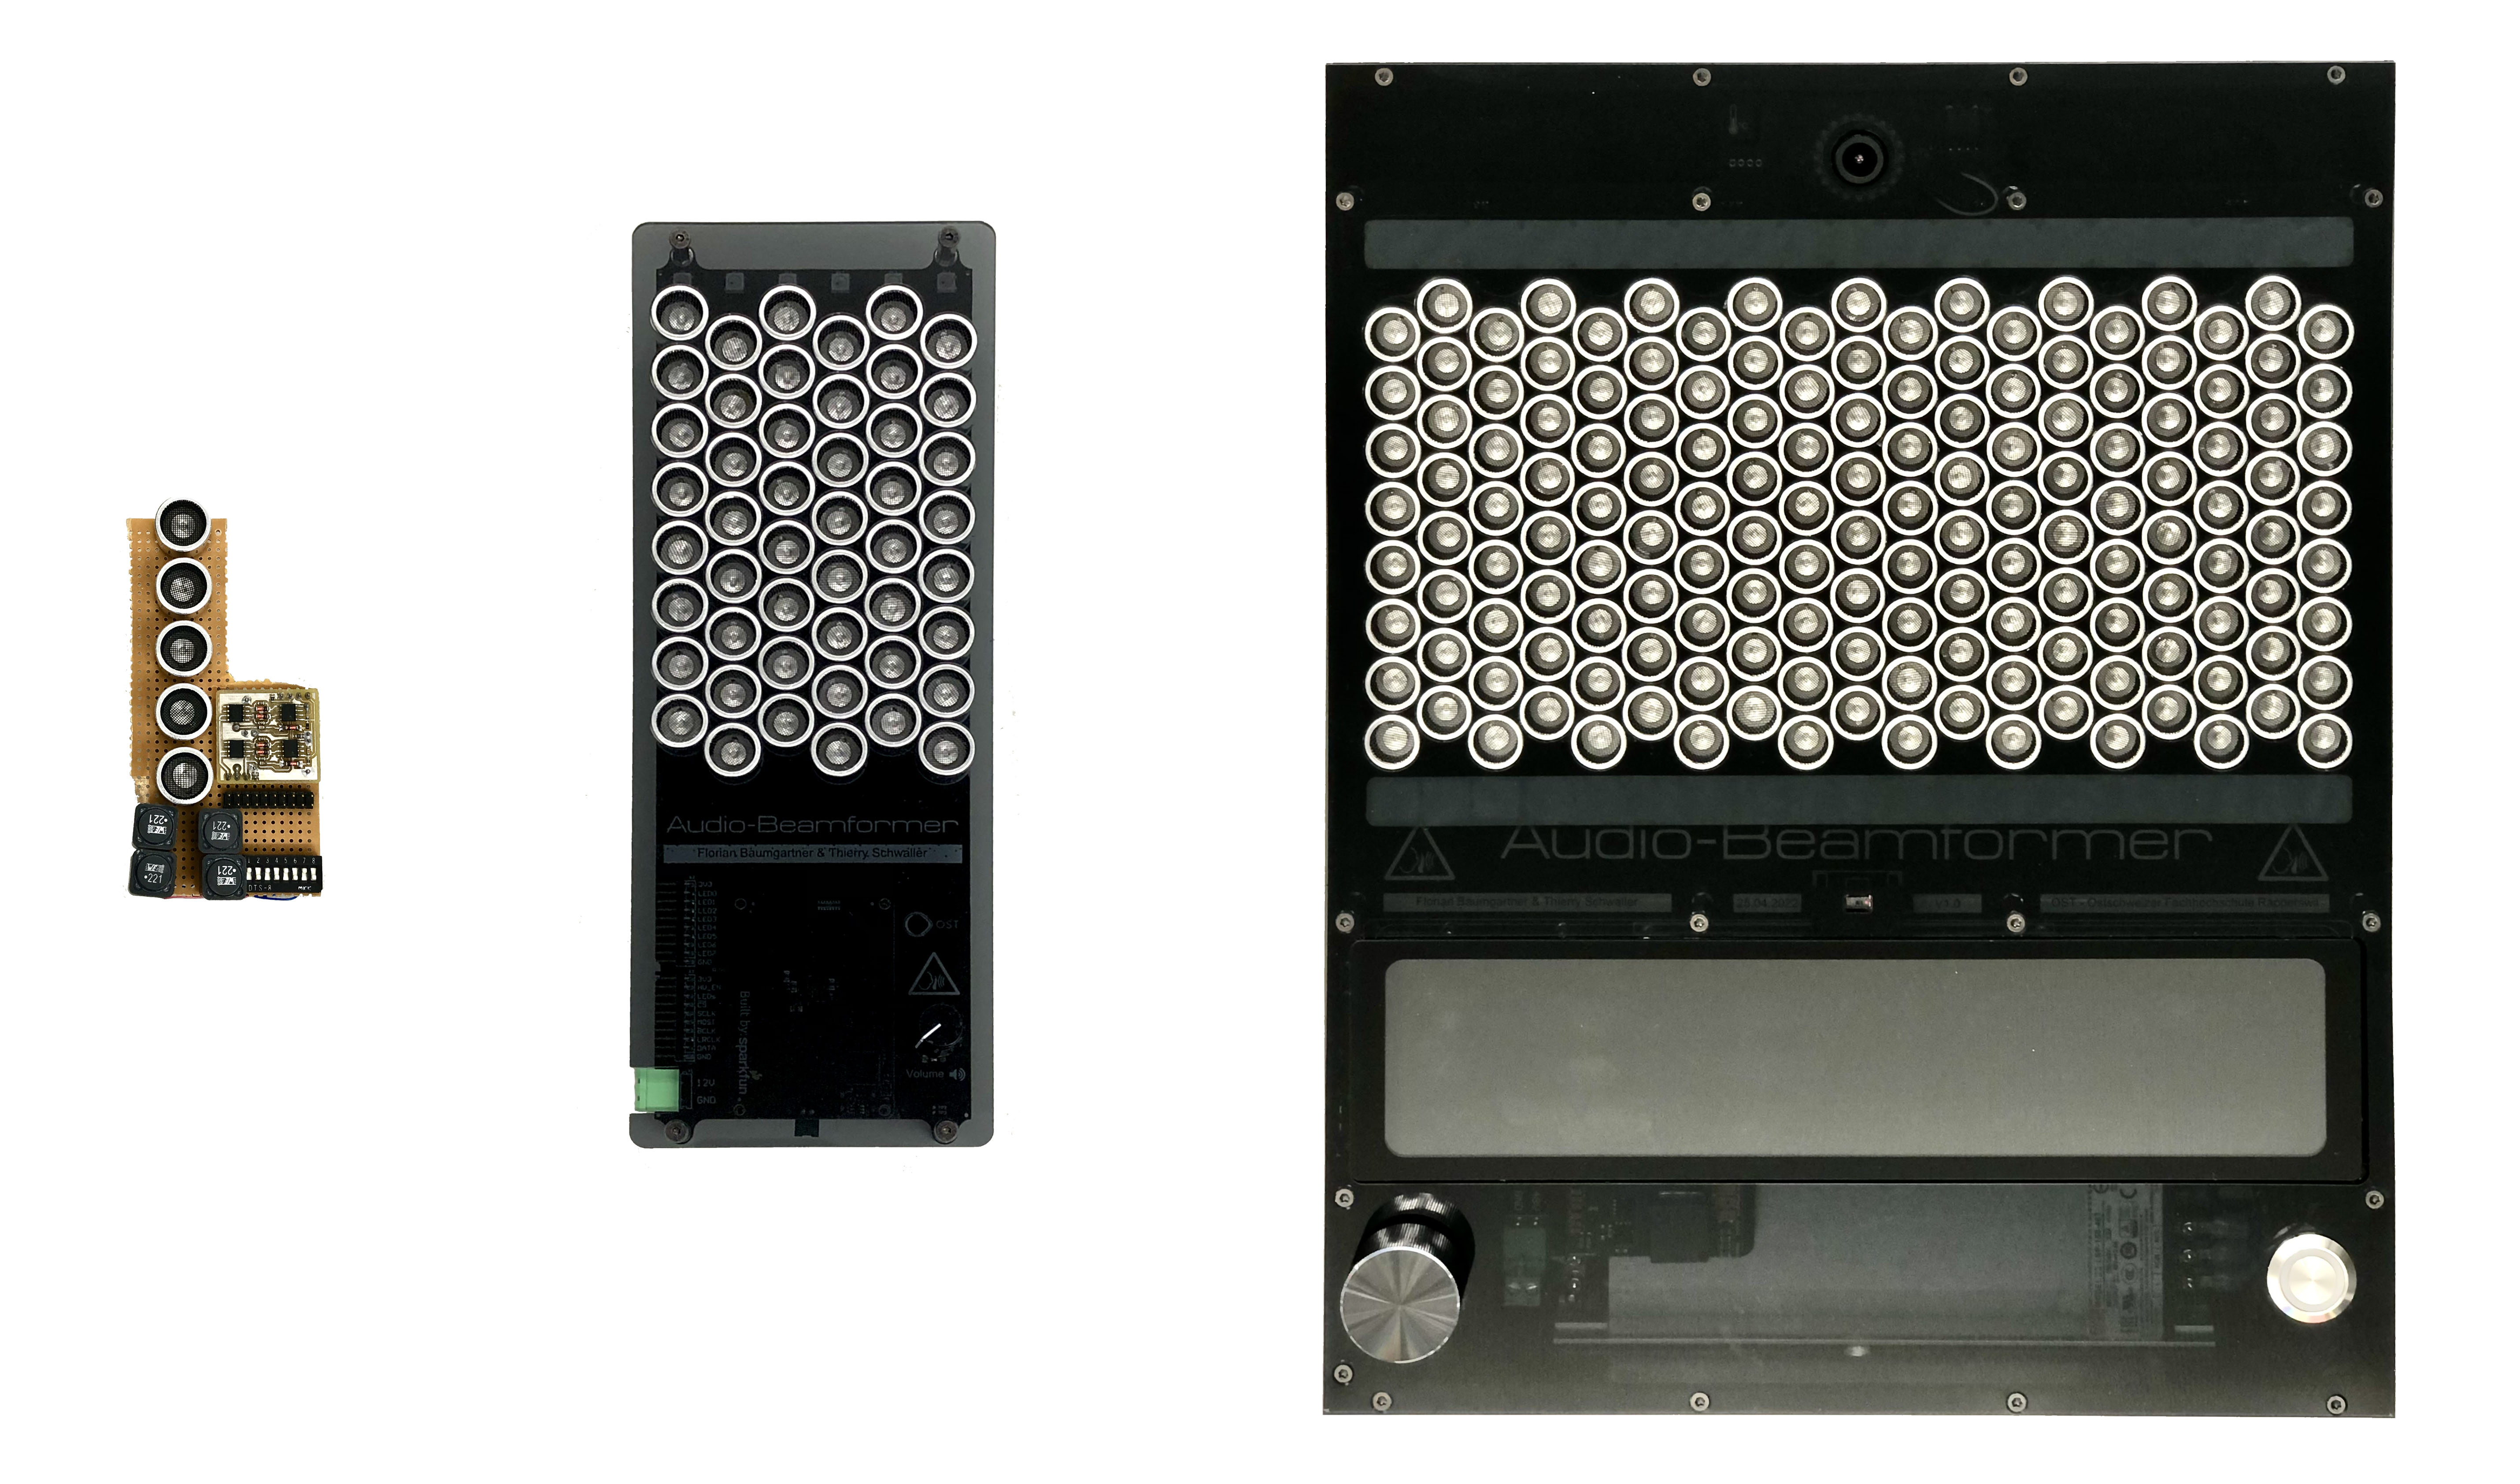
\includegraphics[width=\textwidth]{images/1_Introduction/Approach.jpg}
	\vspace{-0.4cm}
    \caption{Hardware Prototype Revisions}
    \label{fig:prototype_revisions}
\end{figure}


\section{Open Source}
Right from the start it was decided that everything about the project would be released under an open source license. Both of us are huge supporters of open source and believe it will be the future of engineering. Building upon existing libraries and code under open source licenses, allowed us to accelerate the design process. Sometimes open source is considered an act of charity, but in our case, the benefits of using it outweigh any closed source processes. All documents and files for this project can be found on our GitHub page. A short description of all the repositories can be found in the Appendix \ref{Data Archive}.

\chapter{Preliminaries}
\section{Class-D Amplifier}
A Class-D Amplifier, also known as "digital-amplifier" is a very efficient design of a power amplifier most commonly used in audio applications. The main principal is based on a switching output stage (often constructed with \acrshort{mosfet}s) that is driven by a \acrfull{pwm} signal. The switching frequency is much higher than the bandwith of the amplified signal (typically one order of magnitude higher or even more). The most common modulator scheme uses a saw-tooth shaped signal and a comparator to generate the \acrshort{pwm} signal.\\
The output signal then must be low-pass filtered, in order no suppress the high switching noise. This is most usually be done by using a second order LC-Filter at the output. Class-D amplifiers benefit from a low component count and the very high efficiency of up to 90\% and above.

\begin{figure}[h!]
	\centering
	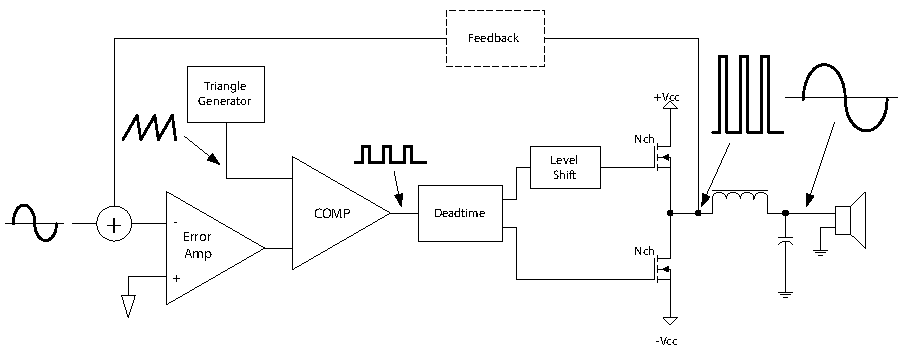
\includegraphics[width=\textwidth]{images/2_Preliminaries/Class-D Amplifier.pdf}
	\vspace{-0.2cm}
    \caption{Typical Class-D Amplifier \cite{analog_class_d_Basics}}
    \label{fig:class_d_amplifier}
\end{figure}
\newpage

\section{Quadrature Amplitude Modulation}\label{2_QAM_sec:QAM}
\acrfull{qam} \cite{nat_skript} is a modulation scheme where an in-phase component $I(t)$ and a quadrature component $Q(t)$ are mixed with orthogonal carriers and then added together, as shown in Figure \ref{2_fig:qam_diagram}. 
\begin{figure}[h!]
    \centering
    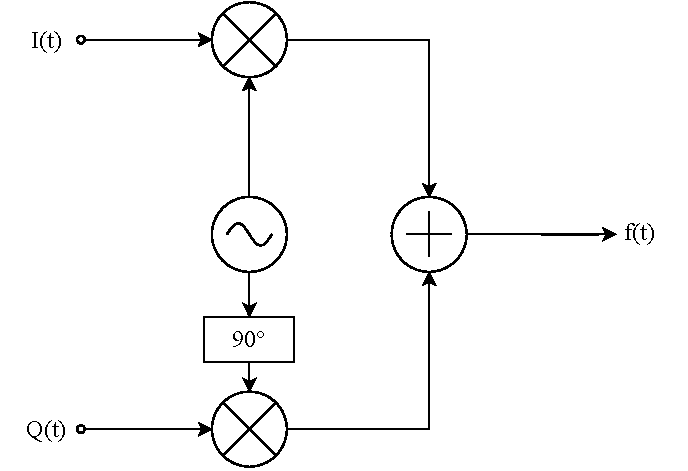
\includegraphics[width=0.5\textwidth]{images/2_Preliminaries/QAM.pdf}
    \caption{Block diagram \acrshort{qam}}
    \label{2_fig:qam_diagram}
\end{figure}

The output signal $f(t)$ can be calculated as 
\begin{equation}
    f(t) = I(t) \sin \left ( \omega_0 t\right ) + Q(t)\underbrace{\sin \left ( \omega_0 t + \frac{\pi}{2} \right)}_{\cos{(\omega_0 t)}}.
\end{equation}
Through the use of some trigonometric identities this can be simplified to 
\begin{equation}
    f(t) = \sqrt{I^2(t) + Q^2(t)} \sin{\left(\omega_0 t + \arctan{ \left ( \frac{Q(t)}{I(t)} \right )}. \right )}
\end{equation}
\section{Piezoelectric Ultrasonic Transducer}
\acrfull{put} emit sound by using the reciprocal piezoelectric effect \cite{air_coupled_ultraonic}. By applying an electric voltage to piezoelectric material it is deformed and therefore produces ultrasound. Electrically a \acrshort{put} is best described by using the Butterworth Van Dyke model, which is shown in Figure \ref{2_fig:butt_dyke_model}.
Of which the impedance response looks like Figure \ref{2_fig:impedance_put}.
\begin{figure}[h!]
    \centering
    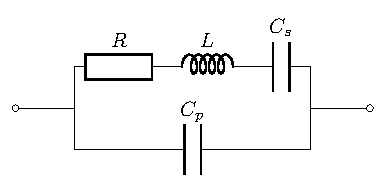
\includegraphics[width=0.5\textwidth]{sections/Van_Dyke_Circuit.pdf}
    \caption{Butterworth van Dyke model}
    \label{2_fig:butt_dyke_model}
\end{figure}
\begin{figure}
    \centering
    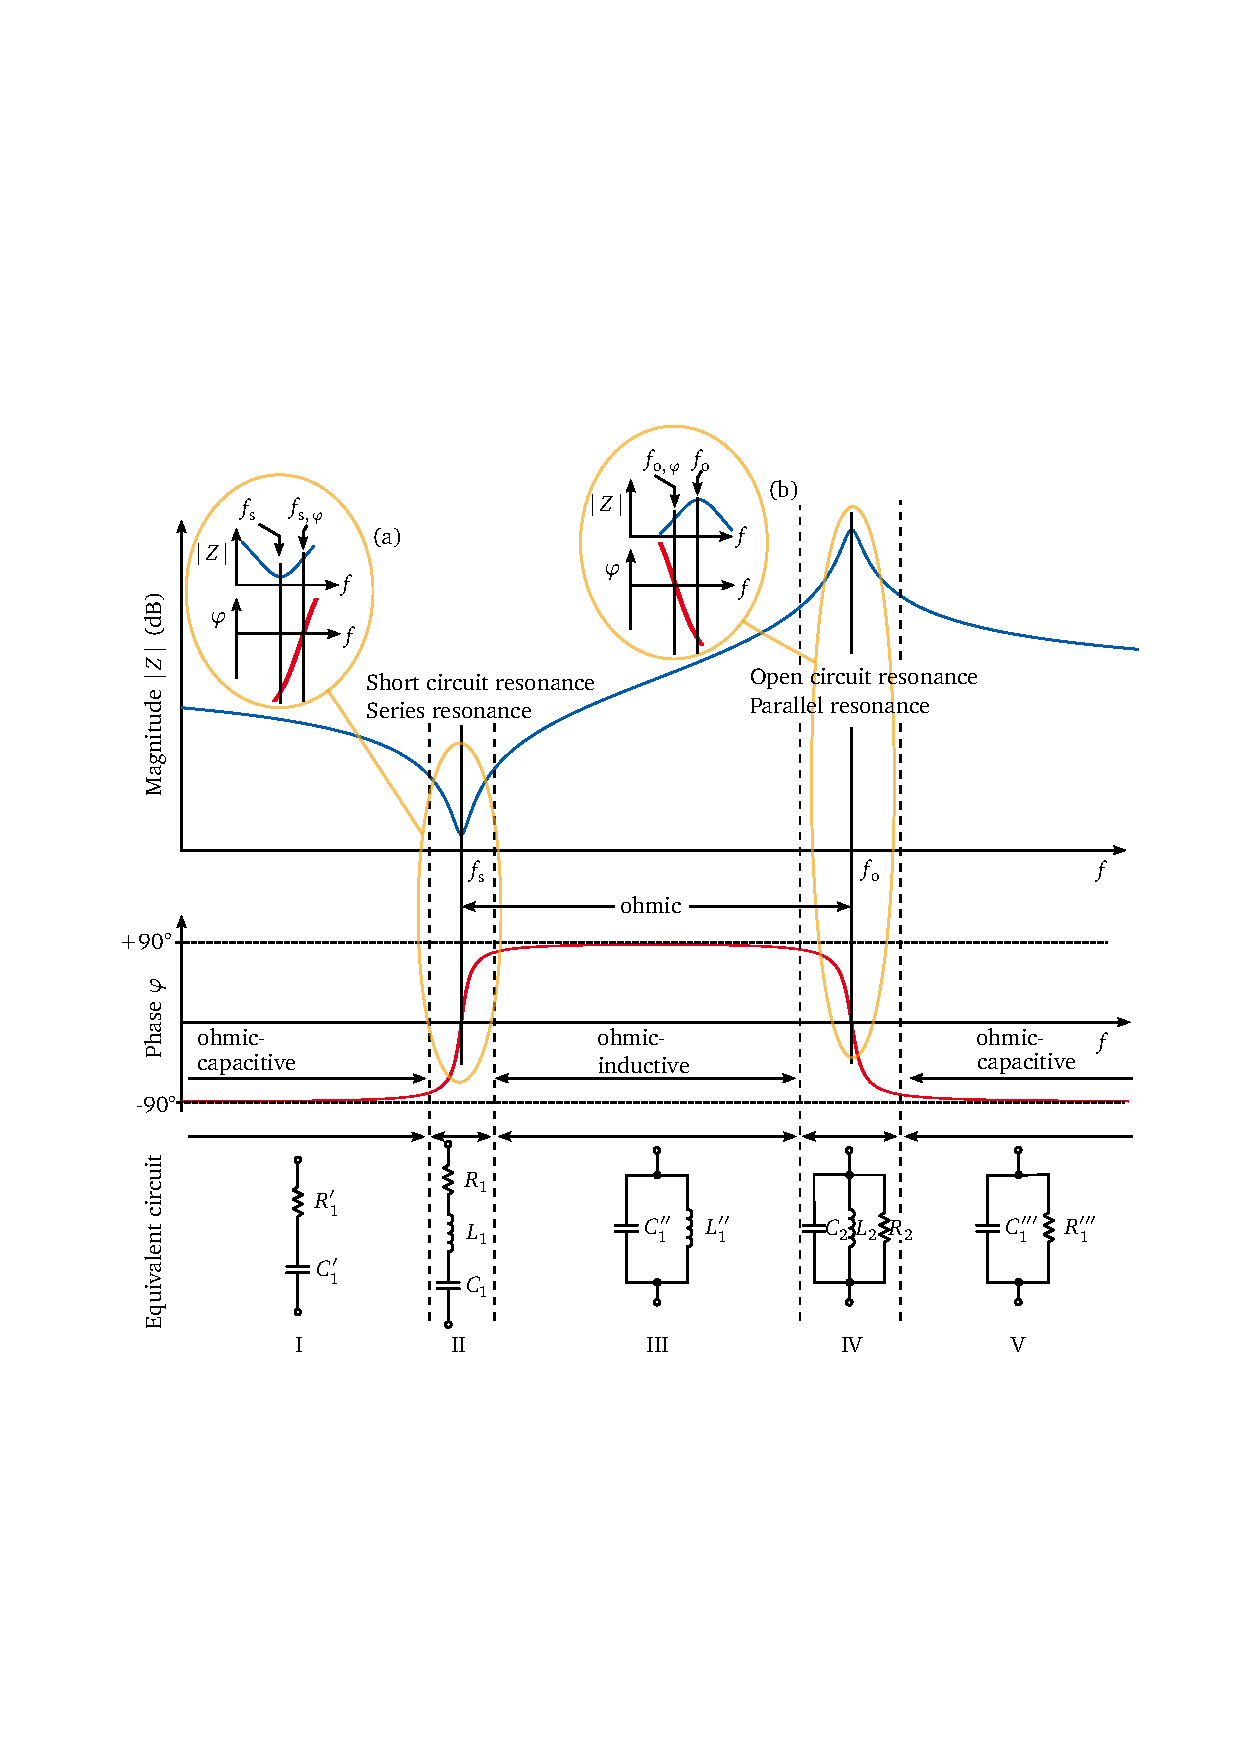
\includegraphics[width=0.85\textwidth]{images/2_Preliminaries/Impedance_PUT.pdf}
    \caption{Magnitude of the impedance response \cite{air_coupled_ultraonic}}
    \label{2_fig:impedance_put}
\end{figure}


\section{Diffraction from slits}
The principle of Huygens-Fresnel \cite{physik_skript} states that every element on a wave surface can be viewed as a center of a spherical wave. Even if this is physically viewed not entirely correct, this provides a good model through which the wave changes in time can be calculated. This principle will be used to calculate the diffraction of waves on slits.

The calculations for the diffraction are only made in the far-field. 
\subsection{Single-Slit Diffraction}\label{2_subsec:single_slit}
All the points inside of the slits are viewed, accordingly to the huygens-fresnel principle, as centers of spherical waves. 
If we now want to know the pressure of a wave of frequency $\omega$ at a certain point in space, with distance r and angle $\phi$ to the slit, one can superposition all the points inside of the slit \cite{physik_skript}
\begin{equation}
    p(r, \phi, \omega)  
    = 
    \frac{A}{rs}\int_0^s \cos \left ( \omega t - k r + k x \sin\left ( \phi\right )\right) dx.
\end{equation}
Where A is the amplitude of the wave at the slit, s is the size of the slit and k is the wave number given as
\begin{equation}
    k 
    = 
    \frac{\omega}{c}
\end{equation}
This can be simplified to be
\begin{equation}
     p(r, \phi, \omega) 
     = 
     \frac{A}{r}  \underbrace{\frac{\sin \left ( \frac{ks \sin \phi}{2}\right )}{ \frac{ks \sin \phi}{2}}}_{A_s(\phi,k,s)} \cos \left ( \omega t - k r_s\right ).
     \label{2_eq:single_slid_final}
\end{equation}
The function $A_s(\phi,\omega,s)$ shows how the amplitude varies according to the angle, the frequency and the size of the slid. 

In Figure \ref{2_subfig:single_slid_amp} it is shown how the amplitude over the angle changes with different frequency while the slit size is hold constant at $s = 0.016 \,$m for waves with the speed $343 \,$m/s (speed of sound at 22 degrees Celsius). Additionally Figure \ref{2_subfig:single_slid_pow} shows the power. 
\begin{figure}
    \begin{minipage}{0.49\textwidth}
    \centering
    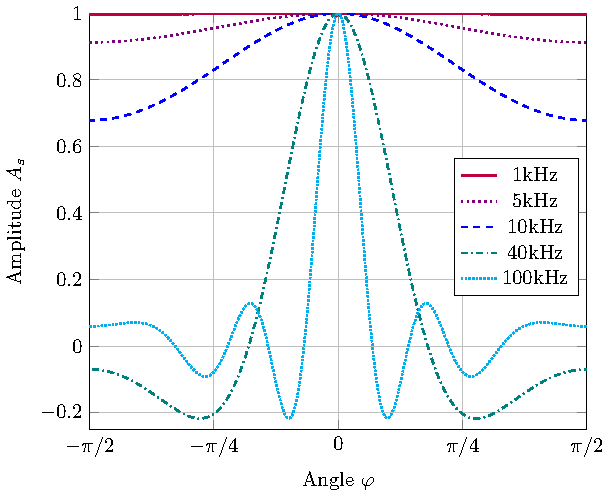
\includegraphics[width=\textwidth]{images/2_Preliminaries/Single_Slid_Frequency.pdf}
    \caption{Amplitude of waves with different frequencies}
    \label{2_subfig:single_slid_amp}
    \end{minipage}
    \begin{minipage}{0.49\textwidth}
    \centering
    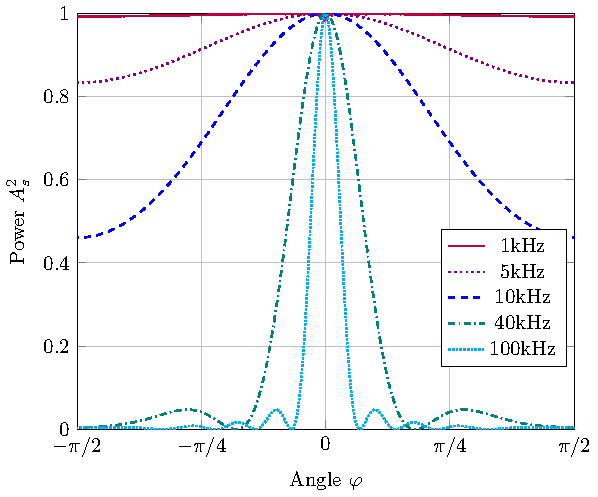
\includegraphics[width=\textwidth]{images/2_Preliminaries/Single_Slid_Frequency_Power.pdf}
    \caption{Amplitude of waves with different frequencies}
     \label{2_subfig:single_slid_pow}
    \end{minipage}
\end{figure}

\subsection{Diffraction on Slits \& Fourier-Transform}\label{2_Acoustics_sec:diffraction_fourier}
Another way to calculate the diffraction pattern of a sound wave on slits is to take a kind of Fourier transform of this slits if the frequency is assume to be $\frac{k x}{2 \pi z}$.

For example in the case with one slit, which has a size of $s$ and and its middle is at the point $(0,0)$ and edges at $(0,\pm s/2)$ the "slit function" $a_s$ would look like
\begin{equation}
     a_s(x) =
    \begin{cases}
      1 & \text{$|x| < \frac{s}{2}$}\\
      0 & \text{else}
     \end{cases}
\end{equation}
Of which the Fourier transform would be
\begin{equation}
    \mathcal{F}\left \{ a_s(x) \right \} = A_s\left ( 2\pi\frac{f x}{c z} \right ) = s\frac{\sin{\left(  \frac{\pi f x s}{c z} \right )}}{\frac{\pi f x s}{c z}} 
\end{equation}
Near the x axis this can be simplified to
\begin{equation}
    \frac{x}{z} = \sin{(\varphi)}
\end{equation}
can be made. This leads to the same formula for the amplitude as seen before in \ref{2_eq:single_slid_final}
\begin{equation}
    A_s(\phi, k, s) = \frac{\sin \left ( \frac{ks \sin \phi}{2}\right )}{ \frac{ks \sin \phi}{2}}.
\end{equation}
\subsection{Multiple Slits Diffraction}
With the fourier transform idea, explained in \ref{2_Acoustics_sec:diffraction_fourier}, the amplitude and power of any multi-slit layout can now easily be calculated. For Z equally sized, $s$, and equally spaced, $d$, grid the pattern can be easily calculated to be
\begin{equation}
     A_s(\phi, k, s, d, Z)
     =
     \frac{\sin \left ( \frac{ks \sin \phi}{2}\right )}{ \frac{ks \sin \phi}{2}} \frac{\sin^2\left( \frac{k d \sin{\varphi}}{2}Z\right )}{\sin^2\left( \frac{k d \sin{\varphi}}{2}\right )}
\end{equation}
Where Z is the number of slits and d is their distance. In Figure \ref{6_fig:multiple_diffraction} an example of a diffraction at multiple slits with different spacing between them is shown.
\begin{figure}
    \centering
    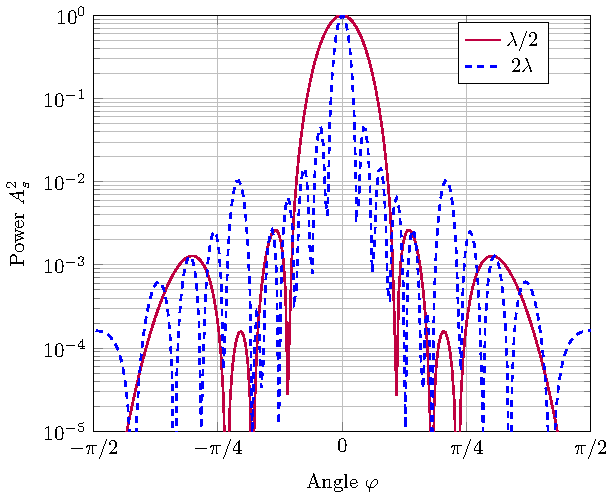
\includegraphics[width=0.7\textwidth]{images/2_Preliminaries/Multiple_Slid_Count.pdf}
    \caption{Diffraction on multiple slits}
    \label{6_fig:multiple_diffraction}
\end{figure}

\newpage
\section{Acoustics}
\subsection{Basics}
A sound wave is a disturbance propagated through  a material (mostly air in acoustics) which causes a variation in pressure.
This disturbance in the ambient pressure is the sound pressure and is proportional to the inverse of the squared distance to the source.\cite{BERANEK20121}
\begin{equation}\label{2_Acoustics_eq:Pressure_sphere}
    p(r) \propto \frac{1}{r^2}.
\end{equation}
To get a better feeling for sound pressure in Table \ref{2_Acoustics_tab:Sound_pressure_level} are some examples of different sound sources, distances and their sound pressure. \cite{rossing1990science}
\begin{center}
\begin{table}[h!]
    \centering
    \begin{tabular}{| c | c | c | c |} 
     \hline 
     Sound source & Distance & Sound Pressure [Pa] & SPL [dB ref. 20$\mu$Pa] \\ 
     \hline
     Jet takeoff & 60$\,$m & 20 & 120 \\  
     Loud shouting & 1.5$\,$m & 2 & 100 \\
     Busy street & - & 0.2 & 80 \\
     Normal conversation & 1$\,$m & 0.02 & 60 \\
     Hearing threshold & - & 0.00002 & 0 \\
      \hline
    \end{tabular}
    \caption{Sound sources and their respective sound pressure (level)}
    \label{2_Acoustics_tab:Sound_pressure_level}
\end{table}
\end{center}
Additionally the sound pressure level (SPL) $L_p$ is displayed. It is the logarithmic measure of sound pressure $p$ relative to a reference value $p_0$.
\begin{equation}
    L_p 
    =
    20 \log_{10} \left ( \frac{p}{p_0} \right ) [dB].
\end{equation}
Mostly this reference value is picked to be $20 \, \mu\text{Pa}$ which is the hearing threshold for humans. \cite{rossing1990science}
\subsection{Sound Power}
The sound power is the total sound energy emitted by a loudspeaker. Often instead of the sound power the sound power level is used. This sound power level $L_W$ is the logarithmic measure of sound power $P$ relative to a reference power $P_0$
\begin{equation}
    L_W = 10\log_{10} \left (  \frac{P}{P_0} \right ) [dB].
\end{equation}
The reference power is often chosen to be $1 \, \text{pW}$. \cite{rossing1990science}
\subsection{Directivity}
In this application specially the directivity of a sound source is of high importance, due to the goal of creating a highly directional beam. 
The directivity of s a sound source is expressed as its directivity factor $Q_D$. It is definded as \cite{DirectivityIndices}
\begin{equation}\label{2_Acoustics_eq:Directivity}
    Q_D = \frac{|p_{axis}|^2}{\rho_0 c}\frac{4 \pi r^2}{W} = \frac{4 \pi p_{rms}^2}{2\pi\int_0^{\pi}p^2_{rms}(\theta)\sin{\theta}d\theta} 
\end{equation}
\subsection{Sound Power Level vs. Sound Pressure Level}
The sound pressure level at any point can be calculated through the distance to the source $r$, the sound power level of the source and the directivity and can be calculated, according to \cite{Relationship_Sound_pressure}, as
\begin{equation}\label{2_Acoustics_eq:SPLvSPL}
    L_p = L_W + 10\log_{10}\left( \frac{Q_D}{4 \pi r^2} + \frac{4}{R_c} \right ).
\end{equation}
Where $R_c$ is the room constant given as
\begin{equation}
    R_c = \frac{S\alpha_{av}}{1 - \alpha_{av}} [m^3].
\end{equation}
Here $S$ stands for the volume  and $\alpha_{av}$ is the average absorption coefficient of the room.  If the room is large enough ($S >> 1$) then $R_c >> 1$ follows which means Equation \ref{2_Acoustics_eq:SPLvSPL} can be simplified to
\begin{equation}
     L_p 
     = 
     L_W + 10\log_{10}\left( \frac{Q_D}{4 \pi r^2} \right ) 
     =
     L_W + 10\left ( \log_{10}(Q_D) - \log_{10}(r^2) - \underbrace{\log_{10}(4\pi)}_{\approx 1.1}  \right ). 
\end{equation}
\chapter{Parametric Phased Array}
%\clearpage
\section{Introduction}
Parametric loudspeaker arrays are linear phased transducer arrays, which use the demodulation of ultrasound in air to generate a highly directional and steerable sound source. This effect was first discovered by Westerveld \cite{doi:10.1121/1.1918525} and used in a loudspeaker, the Audio Spotlight, by Masahide Yoneyama and Jun‐ichiroh Fujimoto \cite{doi:10.1121/1.389414}.

Why ultrasound generates a higher directivity is shown in Section \ref{3_sec:directivity}, how the demodulation works in \ref{3_sec:demodulation} and how signal processing tricks can be used to make everything steerable and of better quality is shown in \ref{3_Parametric_array_Sec:Modulation} and \ref{3_Parametric_array_Sec:Array_signal_processing}.
\section{Directivity of Ultrasound Transducers}\label{3_sec:directivity}
As already mentioned ultrasonic transducer produce a highly directional beam. In this chapter the mathematical foundations for this effect will be laid. 
The simplest model of a transducer is to think of it as a slit on which a incoming planar sound wave is diffracted on.\cite{alma99116706330905515} 
The far-field air pressure of a transducer in relation to the angle and the distance to the transducer can therefore be calculated as
\begin{equation}
    p(\varphi,r) 
    = 
    \frac{A}{r} \underbrace{\frac{\sin \left ( \frac{ks \sin \phi}{2}\right )}{ \frac{ks \sin \phi}{2}}}_{D_T(\varphi)}.
\end{equation}
Where the sinc function is better known as the directivity of the transducer. 
\begin{equation}
    D_T(\varphi) = \frac{\sin \left ( \frac{ks \sin \phi}{2}\right )}{ \frac{ks \sin \phi}{2}}
\end{equation}
This directivity for a $k = \frac{40 \, \text{kHz}}{343 \, \text{m/s}}$ and loudspeaker size of $a = 16 \, \text{mm}$ is shown in Figure \ref{2_subfig:single_slid_amp}. It is important to keep in mind that this directivity is just a model and the true directivity of a transducer can vary massively depending on the geometry of the transducers, especially as the angle increases.
\section{Demodulation Process}\label{3_sec:demodulation}
The most fundamental equation for modeling the non linear behaviour of air is the KZK (Khokhlov, Zabalotskaya and Kuznetsov) equation \cite{MIT_Ultrasound} given as
\begin{equation}
    \frac{\partial^2 p}{\partial z \partial \tau} 
    = 
    \frac{c_0}{2} \nabla^2_rp
    + 
    \frac{\delta}{2c_0^3}\frac{\partial^3 p}{\partial \tau^3} 
    + 
    \frac{\beta}{2\rho_0c_0^3}\frac{\partial^2 p^2}{\partial \tau^2}.
\end{equation}
Of which the analytical solutions can not be calculated.
However the solution can be approximated by first solving for the linear ultrasonic field $p_1$ by setting the nonlinear term to zero $\beta = 0$ and then solve for the nonlinear solution $p_2$ the final solution is then the superposition of these two fields $p = p_1 + p_2$.
The ultrasonic field $p_1$ is described by 
\begin{equation}
     \frac{\partial^2 p_1}{\partial z \partial \tau} 
    = 
    \frac{c_0}{2} \nabla^2_rp_1 
    + 
    \frac{\delta}{2c_0^3}\frac{\partial^3 p_1}{\partial \tau^3} 
\end{equation}
and this can now analytically be solved. 
This solution then can be used as an approximation for the non linear part of the equation
\begin{equation}
     \frac{\partial^2 p_2}{\partial z \partial \tau} 
    = 
    \frac{c_0}{2} \nabla^2_rp_2 
    + 
    \frac{\delta}{2c_0^3}\frac{\partial^3 p_2}{\partial \tau^3} 
    + 
    \frac{\beta}{2\rho_0c_0^3}\frac{\partial^2 p_1^2}{\partial \tau^2}
\end{equation}
which can now be solved near the axis analytically.
The resulting function $p_2$ turns out to be 
\begin{equation}
    p_2 = \frac{\beta P_0^2 a^2}{16 \rho_0 \alpha c_0^4 a^2}\frac{d^2}{dt^2} E^2(t)
\end{equation}
Where $E^2(t)$ is the enveloping of the output signal of the transducers. 
This means that the  pressure of the wave in the farfield is proportional to the second derivative of the squared modulated signal.
\begin{equation}
    p_2 \propto \frac{d^2}{dt^2} E^2(t)
\end{equation}
If the pressure now should be the desired audio signal f(t) the envelope of the output signal of the transducers has to be
\begin{equation}
    E(t) = \sqrt{\left ( 1 + m \int \int f(t)dt^2 \right )} =  \sqrt{\left ( 1 +x^2 \right )}.
\end{equation}
But it turns out that this is  impossible to accomplish because of the bandwidth of the ultrasonic transducers.
If $E(t)$ is written as a taylor approximation
\begin{equation}\label{3_eq:ideal_envelope}
    E(t) 
    = 
    \frac{1}{A} \left ( 1 + \frac{1}{2}x - \frac{1}{8}x^2 + \frac{1}{16}x^3 - \dots \right ) 
    =
    1 - \sum_{k=0}^\infty \frac{2}{k+1} \left ( \binom{2k}{k} \right) \left ( -\frac{x}{4}\right )^{k+1}.
\end{equation}
The spectrum $E_T(\omega)$ of the optimal signal is
\begin{equation}
    E_T(\omega) = \frac{1}{A} \left ( 1 + \frac{1}{2}X(w) - \frac{1}{8}\left (X(w) * X(w)\right ) \pm \dots \right ).
\end{equation}
This shows that $E_T(\omega)$ has an infinite bandwidth, because each correlation in frequency, or multiplication in time, doubles the bandwidth.
So an approximation for the envelope has to be found.
\section{Modulation}\label{3_Parametric_array_Sec:Modulation}
\begin{center}
    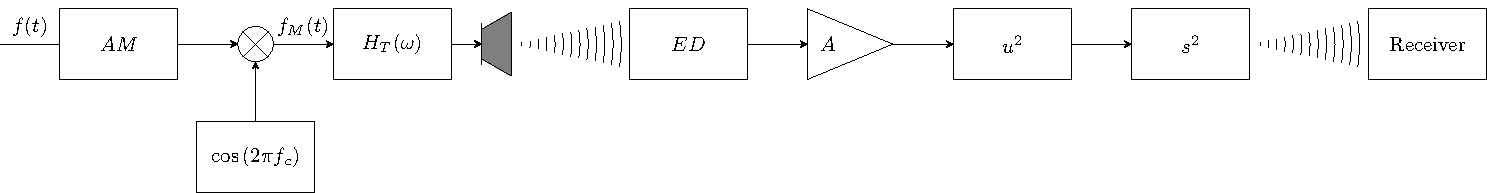
\includegraphics[width=\textwidth]{images/3_Parametric_array/Block_Diagram_Modulation.pdf}
\end{center}
As already mentioned if the ideal envelope, which can be seen in Equation \ref{3_eq:ideal_envelope}, should be emitted by the transducer they would have to have an infinite bandwidth because 
\begin{equation}
    U(\omega) = E_T(\omega) H_T(\omega).
\end{equation}
And because of this an approximation has to be made.
The two approximations that can be made for these envelope function discussed here are AM and MAM. 
\subsection{AM}
One possible approximation is to use normal amplitude modulation. The transmitted signal $g_{AM}(t)$ would be 
\begin{equation}
    g_{AM}(t) = h_T(t) * (1 + mf(t)).
\end{equation}
Often $H_T(\omega)$ is approximated to be $\frac{1}{s^2}$, which would cancel out the two derivatives
\begin{equation}
    f_{RX}(t) 
    = 
    Ag^2_{AM}(t) 
    =
    A(2mf + m^2f^2(t))
    =
   \underbrace{2Amf(t)}_{\text{Signal}} + \underbrace{2Am^2f^2(t)}_{\text{Distortion term}}.
\end{equation}
If the simplification of $H_T(\omega)$ is not made the spectrum of the received signal becomes
\begin{equation}
    F_{RX}(\omega) = 2A(mF(\omega)H(\omega) + m^2(F(\omega)*F(\omega))H(\omega))
\end{equation}
As one can see the modulation index $m$ is squared inside of the distortion term and only linear in the signal. This means that if the modulation index would be chosen small enough the distortion term would vanish, but the power of the signal would also be reduced significantly. 
\subsection{Modified Amplitude Modulation}
As seen if DSBAM is used there is a problematic distortion term. Modified Amplitude Modulation or MAM uses a similar idea to quadrature amplitude modulation to get rid of this problem \cite{MAM_Main_Paper} .
As the inphase component the input signal $1 + mf(t)$ with a DC offset is used and  as the quadrature component the signal $\sqrt{1 - m^2f^2(t)}$ is used. If now the output signal of the modulation $f_M(t)$ is calculated, as described in \ref{2_QAM_sec:QAM}, it turnes out to be
\begin{equation}
    f_M(t) = \sqrt{2 + 2mf(t)} \sin{\left(\omega_0 t + \arctan{ \left ( \frac{\sqrt{1 - m^2f^2(t)}}{1 + mf(t)} \right )} \right )}.
\end{equation}
If $H_T(\omega)$ is now again assumed to be $H_T(\omega) = \frac{1}{\omega^2}$ the signal turns out to be exactly what is should be. 

This would be a perfect modulation method but again because of the square root in the quadrature component this modulation can not be output by the transducers due to their limited bandwidth. However the basic idea still can be used. This is done by approximating the distortion terms with a taylor series
\begin{equation}
    Q(t) 
    = 
    \sqrt{1 - m^2f^2(t)}
    = 
    \sum_{i=0}^\infty \frac{(2i)!}{(1-2i) i!^2 4^i}m^{2i}g^{2i}(t) 
    \approx 
    \sum_{i=0}^m \frac{(2i)!}{(1-2i) i!^2 4^i}m^{2i}g^{2i}(t).
    \label{3_eq:mam_distortion_approx}
\end{equation}
Depending on the frequency response of the transducers the degree of the approximation $m$ can be chosen. The higher the degree of approximation gets the higher the bandwidth of the transducers have to be.
\newpage

\section{Array Signal Processing}\label{3_Parametric_array_Sec:Array_signal_processing}
The theory in this section is mostly taken from the book Fundamentals of Ultrasonic Phased Array \cite{alma99116706330905515}.
\subsection{Phased Array Beam Model}
To explain phenomena such as beamsteering and beamfocusing the phased array beam model has to be introduced.
 \begin{figure}[h!]
     \centering
     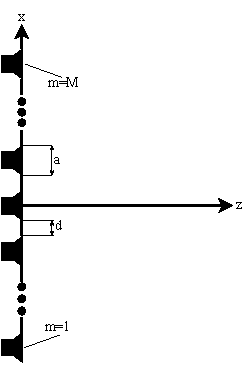
\includegraphics[width=0.4\textwidth]{images/3_Parametric_array/Loudspeaker_Arangement.pdf}
     \caption{Transducer arrangement}
     \label{3_Parametric_array_img:Transducer_Model}
 \end{figure}
Figure \ref{3_Parametric_array_img:Transducer_Model} shows the basic setup of a transducer array with M elements, where M is odd. Where the position of the mth element is given as \cite{alma99116706330905515} 
\begin{equation}\label{3.4_eq:simplified_xm}
    x_m 
    = 
    \left ( \frac{2m -1 - M}{2} \right ) \underbrace{(d + s)}_{c}
    =
    \left ( \frac{2m -1 - M}{2} \right ) c
\end{equation}
Where d is the distance between the transducers, a is the size of the transducers and c is known as the pinch of the array. 
The far field pressure of a single element can be calculated as \cite{alma99116706330905515}
\begin{equation}
    p_m(\textbf{x},\omega) 
    =
    \underbrace{\rho c V_0 \frac{k b}{N} \sqrt{\frac{2}{\pi i}}}_{C} D(\varphi_{m}) \frac{e^{j k b \Bar{r_m}}}{\sqrt{k b \Bar{r_m}}}  
\end{equation}
Where
\begin{equation}
    \Bar{r_m} 
    = 
    \sqrt{\left ( \frac{x}{b} - \frac{e_m}{b}\right )^2 + \left ( \frac{z}{b} \right )^2}
\end{equation}
and 
\begin{equation}
    \varphi_m = \sin^{-1}{\left ( \frac{x - e_m}{b \Bar{r_m}} \right )}
\end{equation}
If now each elements gets its own weighting factor $C_m$ and a phase delay $\Delta t_m$ the pressure at position $\Vec{x}$ of a wave with the frequency $\omega$ can be calulated as 
\begin{equation}
    p(\Vec{x},\omega) 
    = 
    \sum_{i=0}^M C_m e^{j\omega \Delta t_m} \underbrace{C D(\varphi_{m}) \frac{e^{j k b \Bar{r_m}}}{\sqrt{k b \Bar{r_m}}}}_{ p_m(\textbf{x},\omega)} 
\end{equation}
\subsubsection{Far Field}
If only the far field is of interest. Then $\Bar{r}_{m}$ can be simplified to \cite{alma99116706330905515}
\begin{equation}
    \Bar{r}_{m} = R - e_m \sin{\varphi}
\end{equation}
and $\varphi_m$ to
\begin{equation}
    \varphi_m = \varphi.
\end{equation}
So the pressure can be approximately written as
\begin{align}
    p(R,\varphi,\omega) 
    &= 
    C D(\varphi) \sum_{i=0}^M C_m e^{j\omega \Delta t_m} \underbrace{\frac{e^{j k R}}{\sqrt{k R}}}_{P(R)}e^{-jke_m\sin{(\varphi)}} \\
    &= 
    C D(\varphi) P(R) \sum_{i=0}^M C_m e^{j\omega \Delta t_m} e^{-jke_m\sin{(\varphi)}}
\end{align}
Or with \ref{3.4_eq:simplified_xm} as
\begin{equation}
    p(R,\varphi,\omega) 
    = 
    C D(\varphi) P(R) \underbrace{\sum_{i=0}^M C_m e^{j (\omega \Delta t_m -k \left ( \frac{2m -1 - M}{2} \right )s \sin{(\varphi)} )}}_{D_S(\bm{C}, \bm{\Delta t} , \varphi)}
    \label{3_eq:beam_model_final}
\end{equation}
This is the main model used to explain the directivity pattern of linear phased arrays and with using different weights $C_m$ and delays $t_m$ the behaviour can be explored. The sum can be understood as a directivity $D_s$ introduced by the delays and the weighting. 

As an example the weights $C_m = 1$ and $\Delta t_m = 0$ are set to which leads to
\begin{equation}
   D_s(\phi)
    = 
    e^{jks\left ( \frac{M+1}{2} \right )\sin{\phi} } \sum_{m=1}^M \left ( e^{-jks \sin{(\varphi)}} \right ) ^ m 
\end{equation}
This can be seen as a geometric series which can be written as 
\begin{align}
   \sum_{m=1}^M \left ( e^{-jks \sin{(\varphi)}} \right ) ^ m
    &= 
     e^{-jks \sin{(\varphi)}}\frac{1 - e^{-jks \sin{(\varphi) M }}}{1 - e^{-jks \sin{(\varphi)}}} \\
     &=
     e^{-jks\left ( \frac{M + 1}{2}\right ) \sin{(\varphi)}} \frac{\sin{\frac{Mks\sin{(\phi)}}{2}}}{\sin{\frac{ks\sin{(\varphi)}}{2}}}
\end{align}
So the array directivity  in relation to $R$,$\phi$ and $\omega$ can be described as
\begin{equation}
    D_s(\phi) 
    = 
    \frac{\sin{\frac{Mks\sin{(\phi)}}{2}}}{\sin{\frac{ks\sin{(\varphi)}}{2}}}
    \label{3_eq:directivity_no_delay}
\end{equation}
Since $k = \frac{2\pi}{\lambda}$, if $s = \lambda$ the directivity turnes out to be
\begin{equation}
    D_s(\phi) 
    = 
    \frac{\sin{\left ( M\pi\sin{(\phi)} \right )} }{ \sin{\left ( \pi\sin{(\varphi)}\right )}}
\end{equation}
in which the numerator and the denominator are only equal at zero and $2\pi$. So there is only one main lobe in the range between $-\pi/2$ and $\pi/2$. If this is not the case there are multiple lobes with the size of the main lobe.
\begin{figure}
    \begin{minipage}{0.49\textwidth}
    \centering
    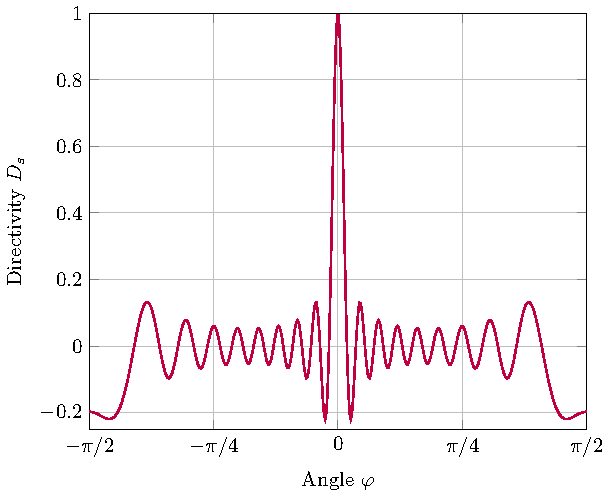
\includegraphics[width=\textwidth]{images/3_Parametric_array/Directivity_NoSteer_Lambda.pdf}
    \caption{Array directivity $s = \lambda$}
    \label{3_subfig:directivity_no_steer_lambda}
    \end{minipage}
    \begin{minipage}{0.49\textwidth}
    \centering
    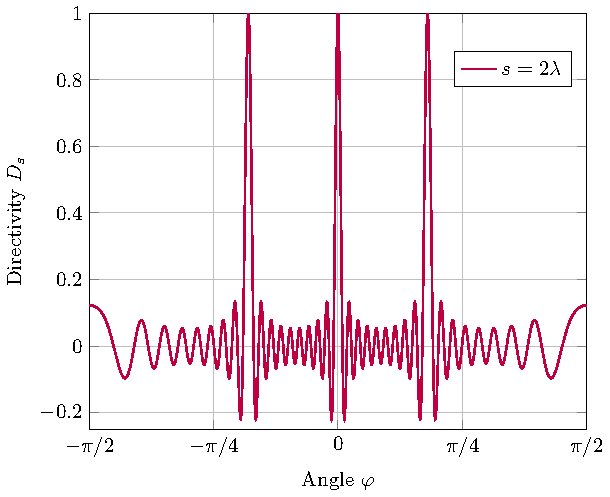
\includegraphics[width=\textwidth]{images/3_Parametric_array/Directivity_NoSteer_2Lambda.pdf}
    \caption{Array directivity $s = 2\lambda$}
     \label{3_subfig:directivity_no_steer_2lambda}
    \end{minipage}
\end{figure}

\subsection{Array Beamsteering}
The basic idea of beam steering is to delay the different channels in such a way that the wave fronts create a certain angle. This can be seen graphicaly in Figure \ref{3_fig:basic_idea_beamforming}.
\begin{figure}
    \centering
    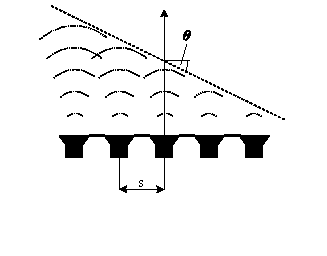
\includegraphics[trim=0mm 7mm 0mm 0mm, width=0.8\textwidth]{images/3_Parametric_array/Beamforming.pdf}
    \caption{Basic idea beamforming}
    \label{3_fig:basic_idea_beamforming}
\end{figure}
If the delays
\begin{equation}
    \Delta t_m = \frac{s \sin{\theta}}{c} \left ( \frac{2m - 1 - M}{2}\right ),
\end{equation}
where $\theta$ is the angle to steer and the weights $C_m = 1$ are inserted into Equation \ref{3_eq:beam_model_final}  
the array directivity $D_S$, after some algebra, is given as \cite{alma99116706330905515}
\begin{equation}
    D_S(1, \bm{\Delta t} , \varphi) 
    = 
    \frac{\sin{\frac{Mks(\sin{(\phi)} - \sin{(\theta)})}{2}}}{M\sin{\frac{ks(\sin{(\varphi)} - \sin{(\theta)})}{2}}}.
\end{equation}
This shows that the beamsteering just moves the the directivity calculated in \ref{3_eq:directivity_no_delay} around.  
This can be seen in Figure \ref{3_fig:directivity_beamsteering} for different steering angles.  
\begin{figure}
    \centering
    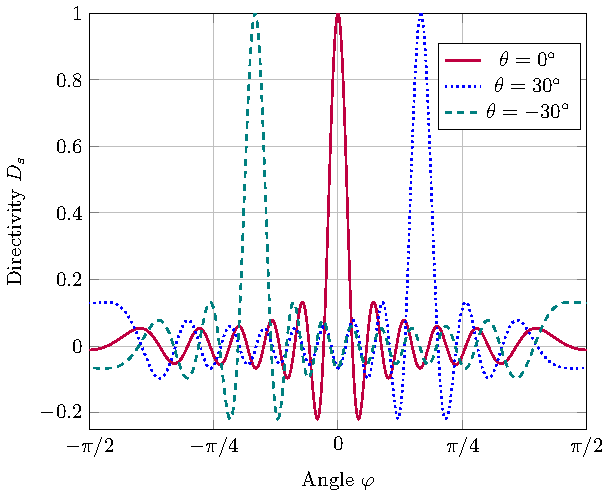
\includegraphics[width=0.7\textwidth]{images/3_Parametric_array/Directivity_Steer.pdf}
    \caption{Array directivity with different steering angles}
    \label{3_fig:directivity_beamsteering}
\end{figure}
\subsection{Beamfocusing}
To focus the beam at a certain radius $R_0$ the delays have to be chosen as
\begin{equation}
    \Delta t_m = \frac{s^2}{2R_0c}(m-1)(M-m).
\end{equation}
This generates delays which are shaped like a parabolic mirror which ensure that the waves exactly meet at the focus point, like shown in Figure \ref{3_fig:beamfocusing}.
\begin{figure}
    \centering
    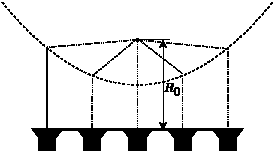
\includegraphics[width=0.7\textwidth]{images/3_Parametric_array/Beamfocusing.pdf}
    \caption{Basic idea beam focusing}
    \label{3_fig:beamfocusing}
\end{figure}
\subsection{Array Amplitude Weighting}
As explained in \ref{2_Acoustics_sec:diffraction_fourier} the diffraction process of a grid can be calculated via the fourier transform. If an array of transducers are used the function f(x) is a rectangular sequence. If this rectangular sequence is now sampled with a sampling width of $d$ then the signal is a rectangular window known from FIR filters. The main difference is now that the time axis was replaced by a spatial axis.
If now weights are applied to the different channels the rectangular window can be changed to other known windowing function, such as Hamming or Hann, and the same theories will hold for the main and side lobes. However the most used window in array signal processing is the dolph-chebyshev window.  
\subsubsection{Dolph-Chebyshev Window}
The Dolph-Chebyshev Window is a special window which minimizes the so called Chebyshev norm of the side lobes for a given main lobe width. The chebyshev norm is the maximum absolute value
\begin{equation}
    \min_{\omega, \sum \omega = 1} \left \{ \max \left[ | \text{Sidelobes}(W(\omega))\right | ]\right \}.
\end{equation}
The transform of the window can be written as
\begin{equation}
    W(\omega_k) = \frac{\cos{ \left [ M \cos^{-1}{\left ( \beta \cos{ \left (\frac{\pi k}{M} \right )} \right)}\right ]}}{\cosh{\left [ M \cosh^{-1}{\left ( \beta \right ) }\right ]}} \qquad k = 0,1,2, \dots, M-1
\end{equation}
Where M is the number of taps of the window and $\beta$ can be used to control the side lobe level.
The  \acrfull{idft} of $W(\omega_k)$ is now the Dolph-Chebyshev window $w(n)$.
The controlling of the side lobe level is often done by introducing another variable $\alpha$ which is connected to $\beta$ in the following way
\begin{equation}
    \beta = \cosh{\left [ \frac{1}{M} \cosh^{-1}{\left ( 10^{\alpha} \right ) } \right ]}.
\end{equation}
The maximum side lobe level is now given as
\begin{equation}
    \text{Side lobe level} = L_s =  -20\alpha [dB]
\end{equation}
Whereas the main lobe width is given as
\begin{equation}
    \omega_c = 2 \cos^{-1}{ \left ( \frac{1}{x_0} \right )} \qquad x_0 = \cosh{ \left [ \frac{\cosh^{-1}{\left ( 10^{\alpha} \right )}}{M-1}\right ]}.
\end{equation}
One can see that the higher the $\alpha$ is chosen the lower the maximum of the side lobes get, but the main lobe gets wider. \todo{Plot}






\chapter{Design}
\section{Overview}
This section covers the complete development process including the hardware, gateware, software and mechanical design of the project. Important to note is, that the following documentation concentrates only on the final version of the device. Earlier hardware prototypes are not covered due to the lack of relevance.

\subsection{Key Requirements}
The main focus of the development is to design a professional looking, easy to use and eye-catching device for demonstration purposes such as info days. The project name \textit{Audio-Beamformer} has been chosen as it is easy to remember and has potential to be seen as a trademark. 

The following key requirements have been set:
\begin{itemize}
    \item Single power adapter or power cable (e.g. no need of labor power supplies) 
    \item Easy to install (e.g. montage on a camera tripod)
    \item Intuitive to operate via state-of-the-art graphical user interface
    \item Multiple audio streaming sources such as Bluetooth and USB input devices
    \item Great scalability and flexibility of the hardware and software design
\end{itemize}

\subsection{Key Decisions}
In the conceptional phase of the development, several key decisions had to be felt. This contains mainly the signal flow and the division between the processing part on the Raspberry Pi and the \acrshort{fpga}. Further, the question had to be evaluated, if a built-in power supply or an external power adapter is preferred. And most importantly, which type of ultrasonic transducer should be used in the design.
In addition, the overall dimension and scale of the final product had to be discussed. 
In general, most of these decisions were felt by the result of simulations, physical measurements and after extensive discussions.
In the following sections, each part of the project is explained in more detail.


\newpage
\section{Hardware Design}
The hardware of the Audio-Beamformer was designed using Altium Designer 22. The integrated 3D \acrshort{cad} functionality simplified the overall development and lowered the possibility of errors in the design.
The hardware has been improved over several iterations until a final version could be built.\\
The 2-Layer \acrfull{pcb} with the size of 300.0\,mm\;x\;376.0\,mm has been manufactured and assembled by JLCPCB.\\

\begin{figure}[h!]
	\centering
	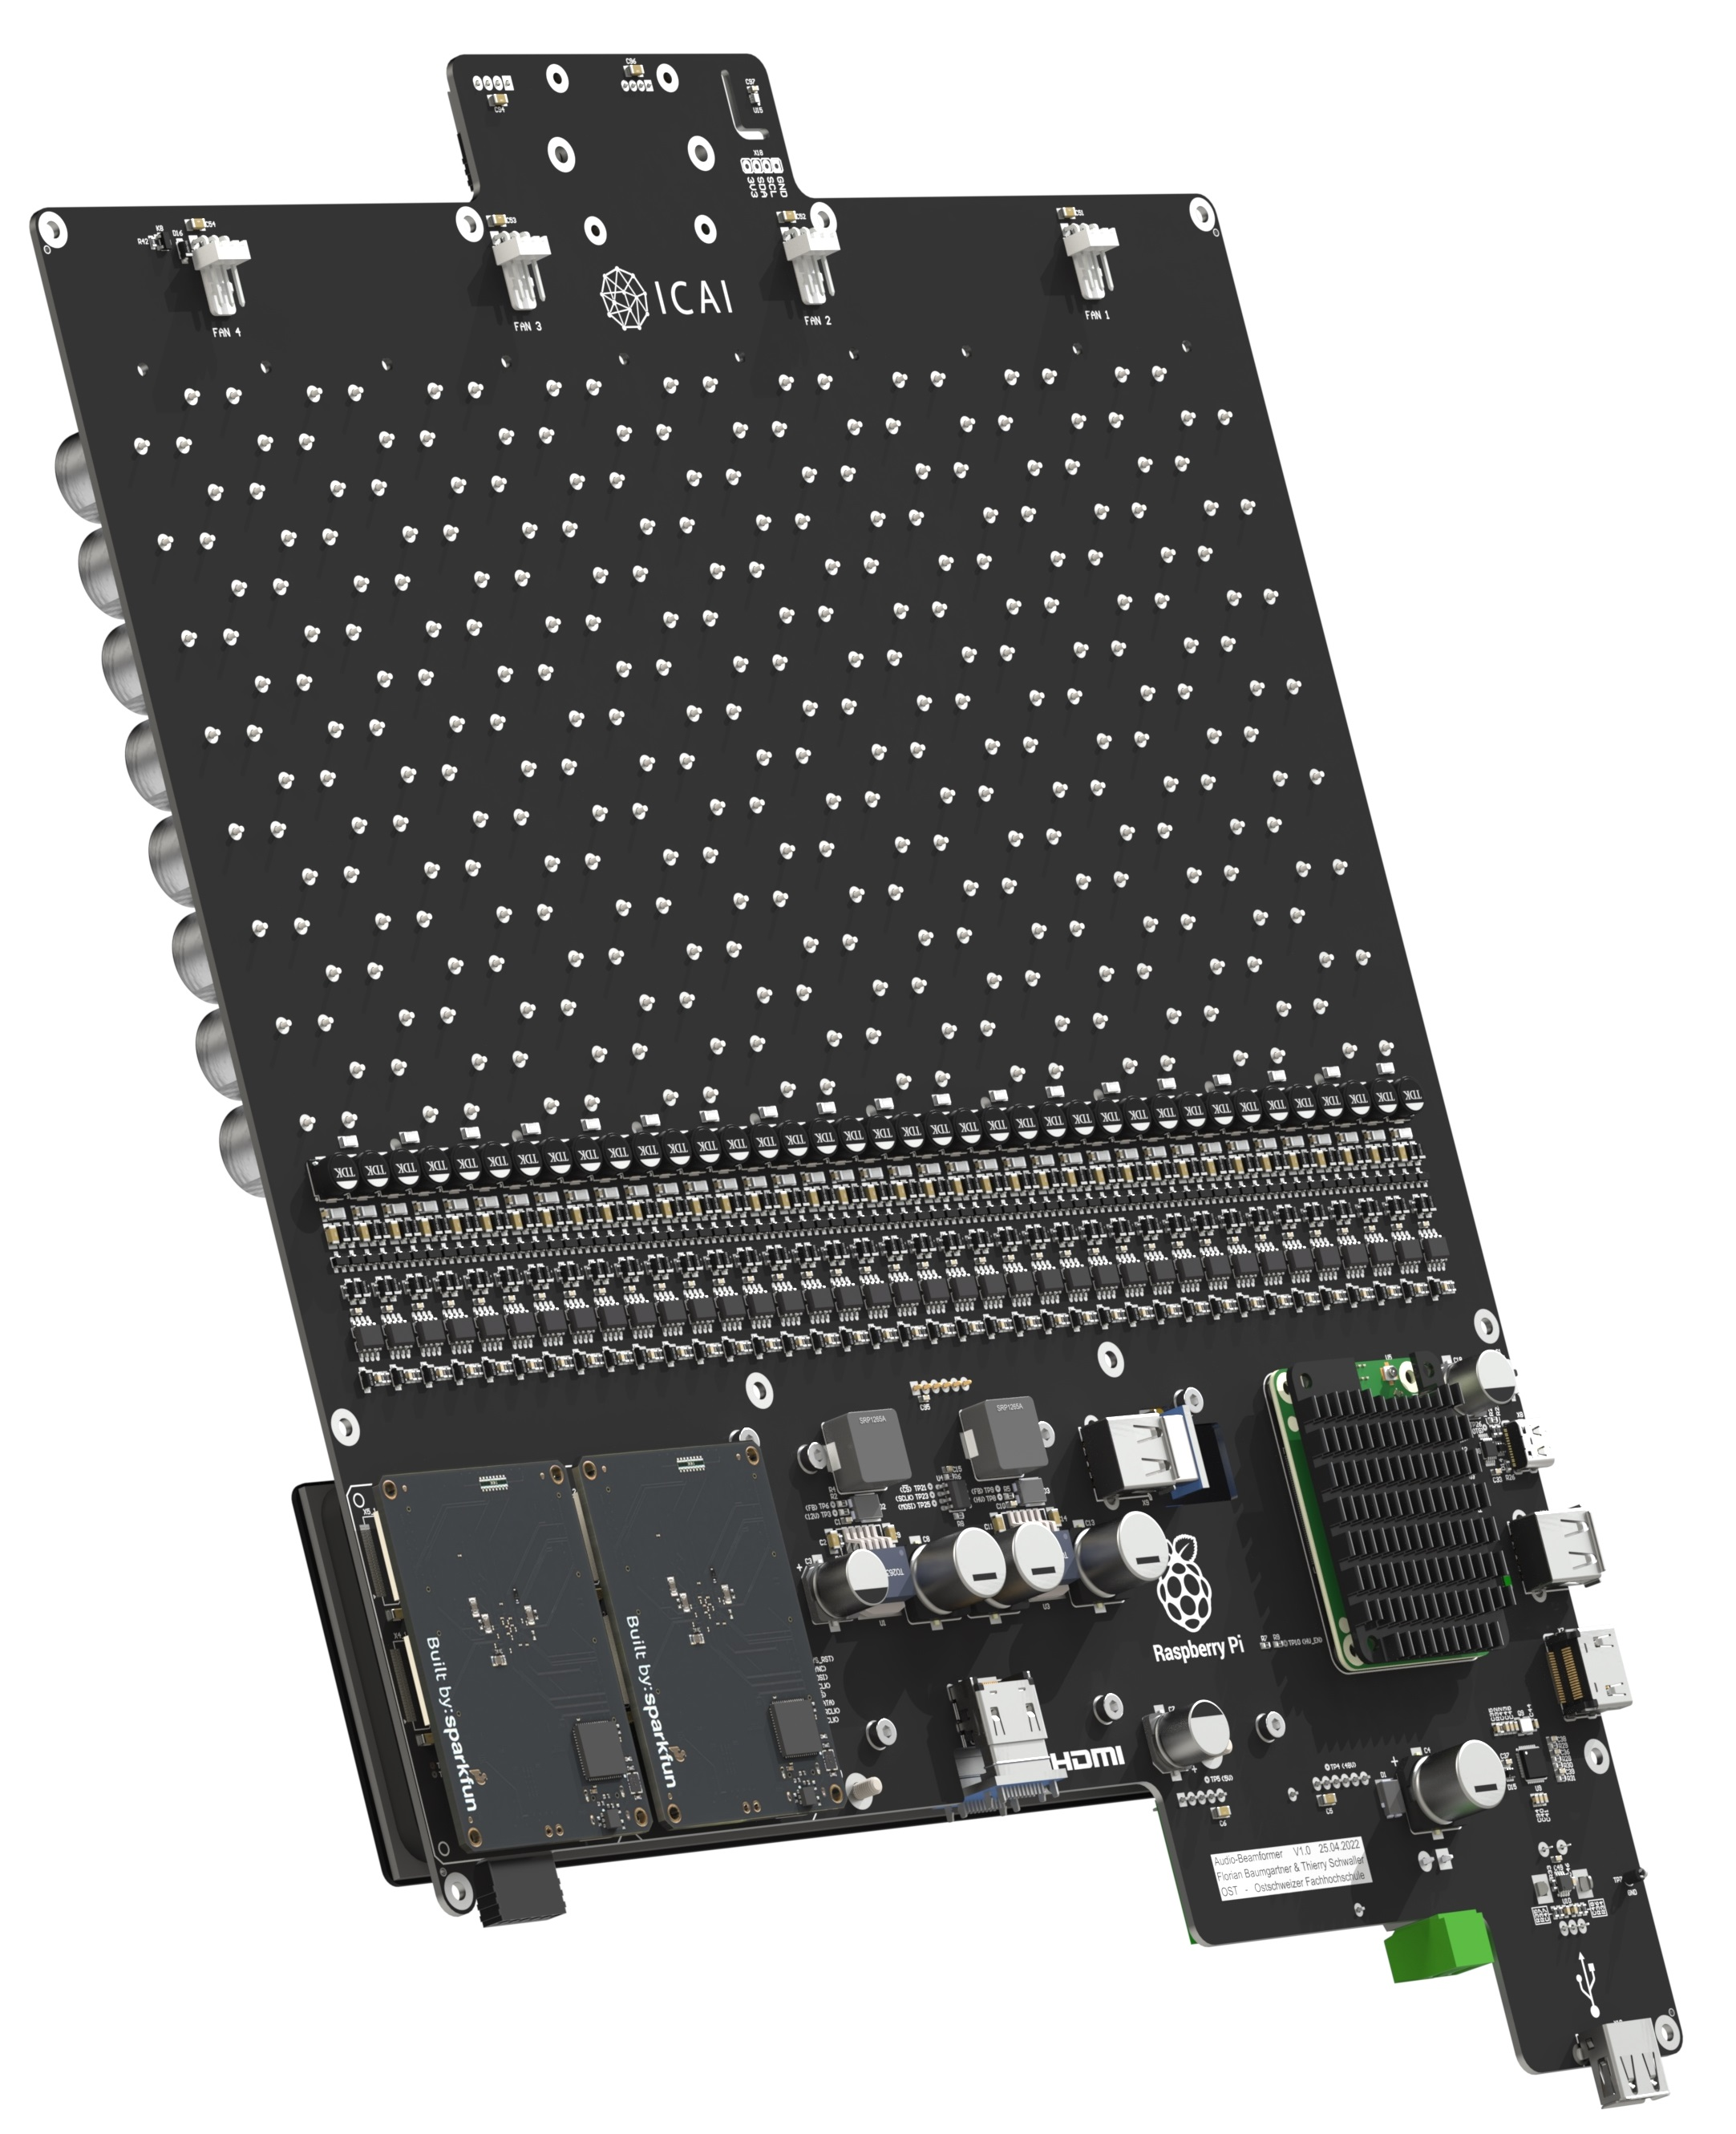
\includegraphics[width=14cm]{images/4_Design/Hardware/Audio-Beamformer_PCB.jpg}
	\vspace{-0.2cm}
    \caption{3D-Render of \acrshort{pcb}}
    \label{fig:pcb_render}
\end{figure}
\newpage

\subsection{Block Diagram}
\begin{figure}[h!]
	\centering
	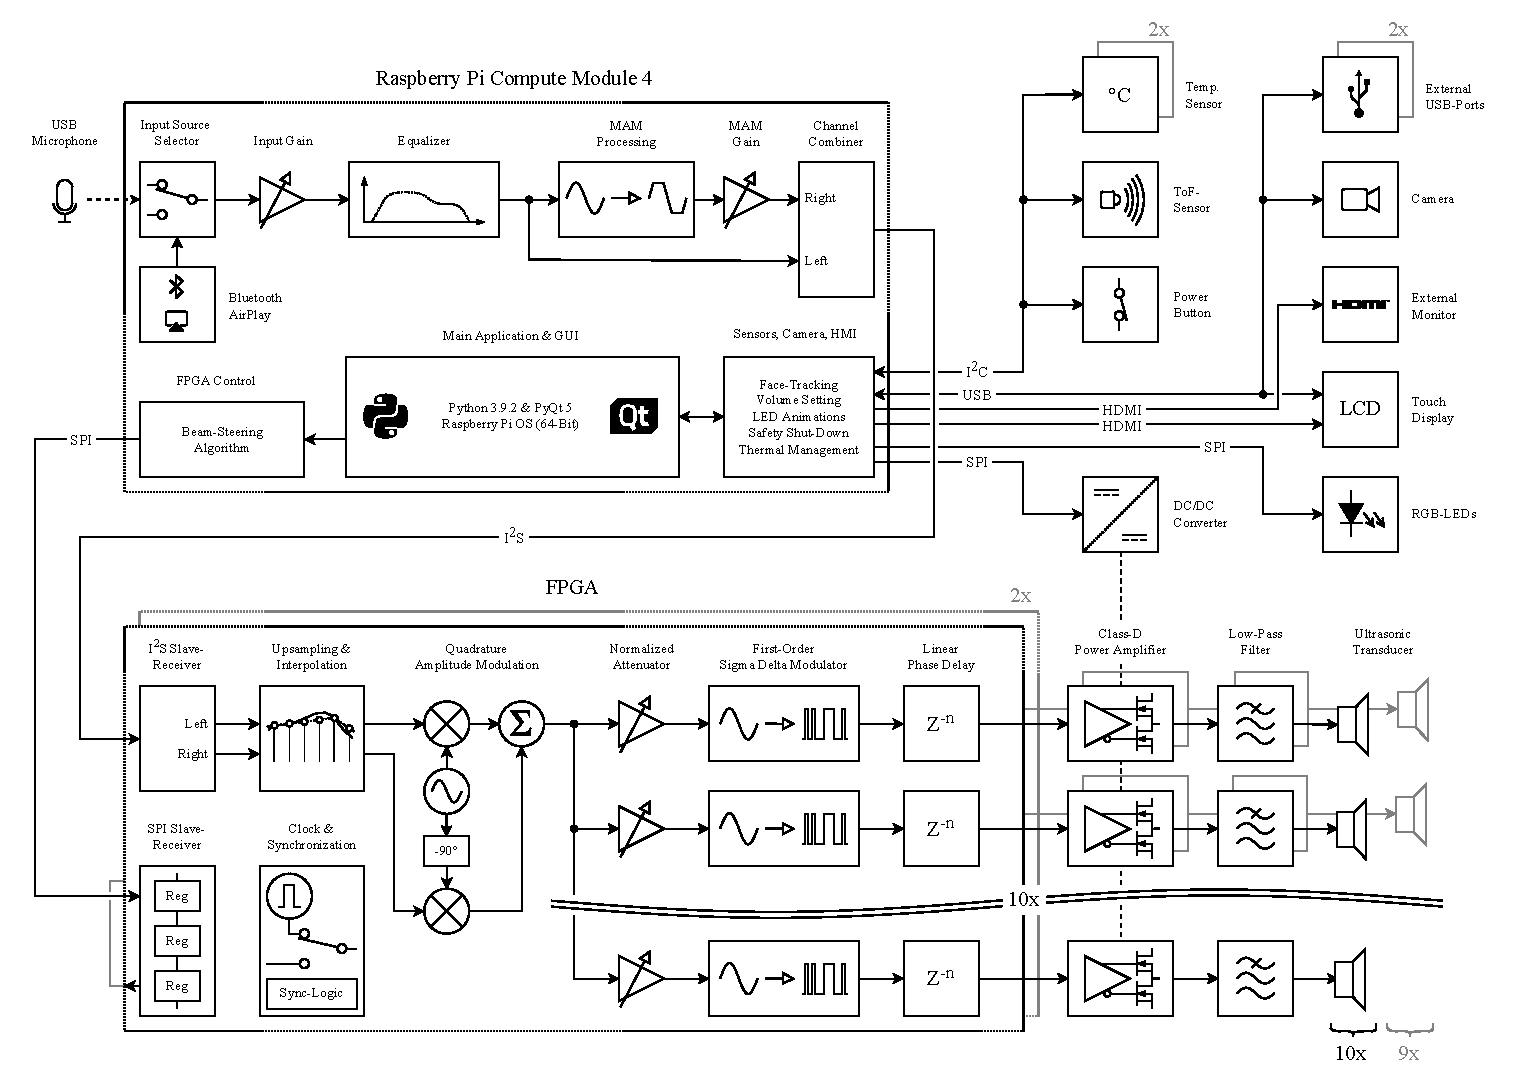
\includegraphics[width=21.5cm, angle=90]{images/4_Design/Hardware/System Block Diagram 2.pdf}
	\vspace{-0.2cm}
    \caption{System Block Diagram}
    \label{fig:hardware-block-diagram}
\end{figure}

\clearpage
\subsection{Power Management}
The Audio-Beamformer is powered directly by mains voltage. As a connector, the widely used C14 (IEC 60320) has been chosen. Because of the metallic casing, protective earth is required. It has been connected directly to the back panel. The main switched mode power supply is made by \textit{Mean Well} and delivers 48\,V \acrshort{dc} and up to 163\,W output power. The LSP-Series is specially designed for low-profile applications and therefore ideal in this use case.\newline
The simplified power management diagram \ref{fig:simplified-power} provides a better overview of how each voltage rail is created.

\begin{figure}[h!]
	\centering
	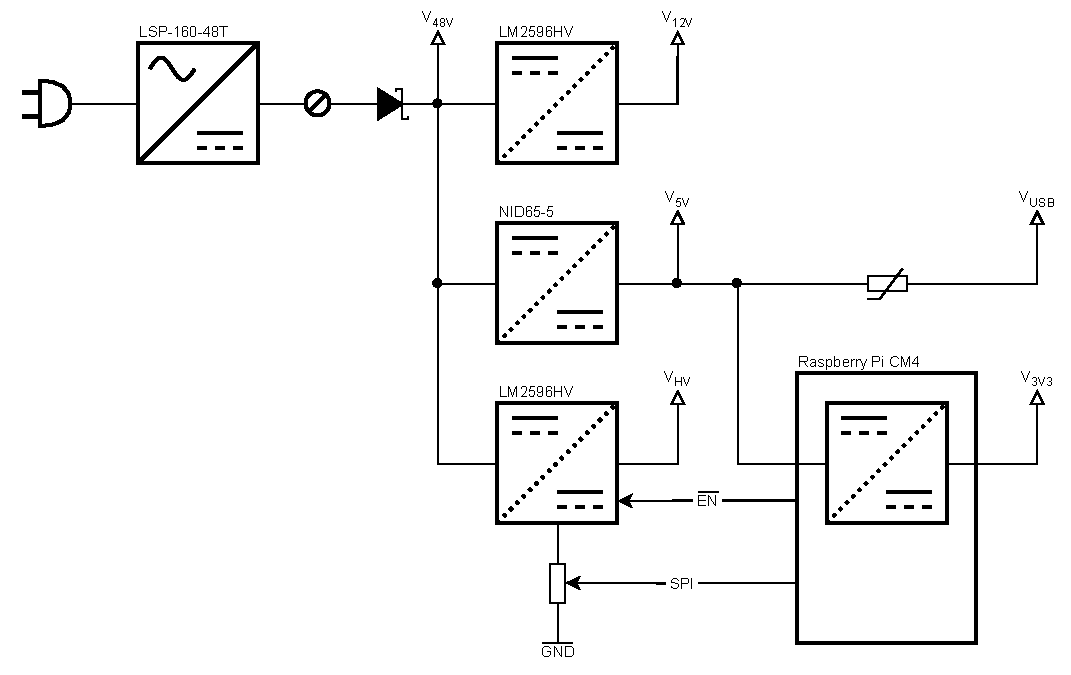
\includegraphics[width=\textwidth]{images/4_Design/Hardware/Power Supply Overview.pdf}
	\vspace{-0.6cm}
    \caption{Simplified Power Management}
    \label{fig:simplified-power}
\end{figure}

As a reversed polarity protection a schottky diode has been placed directly after the input connector. Further \acrshort{dc}-\acrshort{dc} buck converters generate fixed 5\,V (6.5\,A), 12\,V (2.0\,A) and a variable HV rail.


\bigskip
\begin{wrapfigure}{r}{7cm}
    \vspace{-0.6cm}
    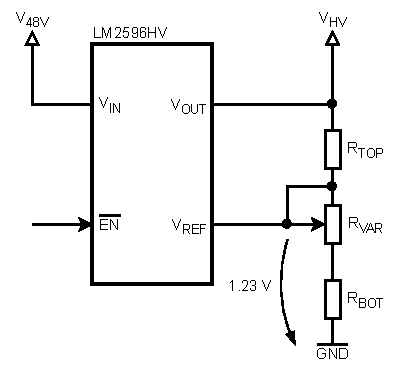
\includegraphics[width=7cm]{images/4_Design/Hardware/Variable Buck-Converter.pdf}
    \vspace{-0.6cm}
    \caption{Variable Buck-Converter}
    \label{fig:variable-buck-converter}
\end{wrapfigure} 
For adjusting the physical output volume of the ultrasonic transducers, the amplifier drive voltage must be changed accordingly. The HV voltage supply can be set between 5.2\,V and 23.5\,V (2.0\,A). This has been achieved by using a digital potentiometer (MCP41010T) which is controlled by an \acrshort{spi}-Interface.\\
For safety reasons, the HV voltage is turned off per default and must be enabled by a physical logic signal provided by the Raspberry Pi.
\clearpage

The output voltage can be calculated as follows

\begin{equation}
    V_{HV}(R_{var}) = \frac{V_{ref}}{R_{bot} + R_{var}} (R_{bot} + R_{top} + R_{var}).
\end{equation}

Where $R_{var}$ is proportional to its 8-bit value (\codeword{0x00} $\cong$ 0\,$\Omega$ and \codeword{0xFF} $\cong$ 10\,k$\Omega$). The reference voltage of the DC-DC buck converter (LM2596HV) is 1.23\,V. The resistor values used in the design are $R_{top}$ = 39\,k$\Omega$, $R_{bot}$ = 2.0\,k$\Omega$ and $R_{var}$ = 10\,k$\Omega$. This leads to the following approximation
 \begin{equation}
    V_{HV}(d) \approx 5.2\,V + d\:\frac{20\,V}{255}.
\end{equation}

\subsection{Raspberry Pi Compute Module 4}
As a main processing platform the Raspberry Pi Compute Module 4 has been chosen due to its powerful quad-core processor and the great software support based on a large community. The exact model used in the design has 4\,GB of \acrshort{ram} and fixed installed 16\,GB of embedded \acrshort{emmc} flash storage. This has the advantage of being more reliable than systems that are dependent on a \acrshort{sd}-Card.
To increase the performance, the Raspberry Pi has been overclocked to 1.0\,GHz. Sufficient cooling is provided by a heat sink and four cooling fans.
The \acrshort{io} operating voltage has been set to 3.3\,V.

\subsection{FPGA} \label{hardware_fpga}
There are two \acrshort{fpga}s used in the design for generating the drive signals for the ultrasonic transducers. Each \acrshort{fpga} is mounted on a development board called \textit{Alchitry Cu}. They are installed as daughter-boards on the main \acrshort{pcb} by high-speed board-to-board connectors. Both \acrshort{fpga}s receive the audio stream via an \acrshort{i2s}-Stream and get controlled by a simple \acrshort{spi}-Protocol in an daisy-chain configuration. More details on this in section \ref{fpga_i2s} and \ref{fpga_spi}.\\
The \acrshort{fpga} boards are powered by 5\,V, because they have an on-board 3.3\,V regulator build-in.


\subsection{Sensors and HMI}
The Audio-Beamformer contains several sensors that are connected by different interfaces to the Raspberry Pi Compute Module. The \acrfull{hmi} enables easy access to change various settings of the device.

\subsubsection{Camera}
To be able to direct the sound towards a specific person, a camera is needed. In this case a \acrshort{usb}-Camera has been chosen since it is easy to connect and does not need any special device drivers. The type \textit{ELP-USB500W02} provides a resolution of 1280\,x\,720 pixels and a frame rate of up to 30\,FPS. The optics used in this application are designed to match the viewing angle of the camera to the maximal beam-steering angle of the Audio-Beamformer. In this particular case, a camera lens with a focal length of 4.2\,mm has been chosen which results in a viewing angle of ca. ±40°.

However the camera had to be slightly modified. On startup, it tries immediately to establish an \acrshort{usb} connection to the host device. If there is no response during the first 500\,ms the camera goes into a power-down/suspend mode. In this state it can't be recognized by the host until it gets power-cycled. This issue has been solved by increasing the RC time constant of the camera internal power-on reset circuitry from 4.7\,ms to ca. 4.7\,s. In addition a schottky diode has been added to guarantee a fast discharge time after powering off the device. This ensures a valid reset-pulse even if the device gets power-cycled very rapidly.

\begin{figure}[h!]
    \centering
    \subfloat[\centering Reset-Circuit]{{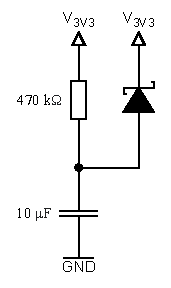
\includegraphics[height=6cm]{images/4_Design/Hardware/Camera Reset-Circuit.pdf}}}
    \qquad
    \subfloat[\centering Location of RC-Circuit]{{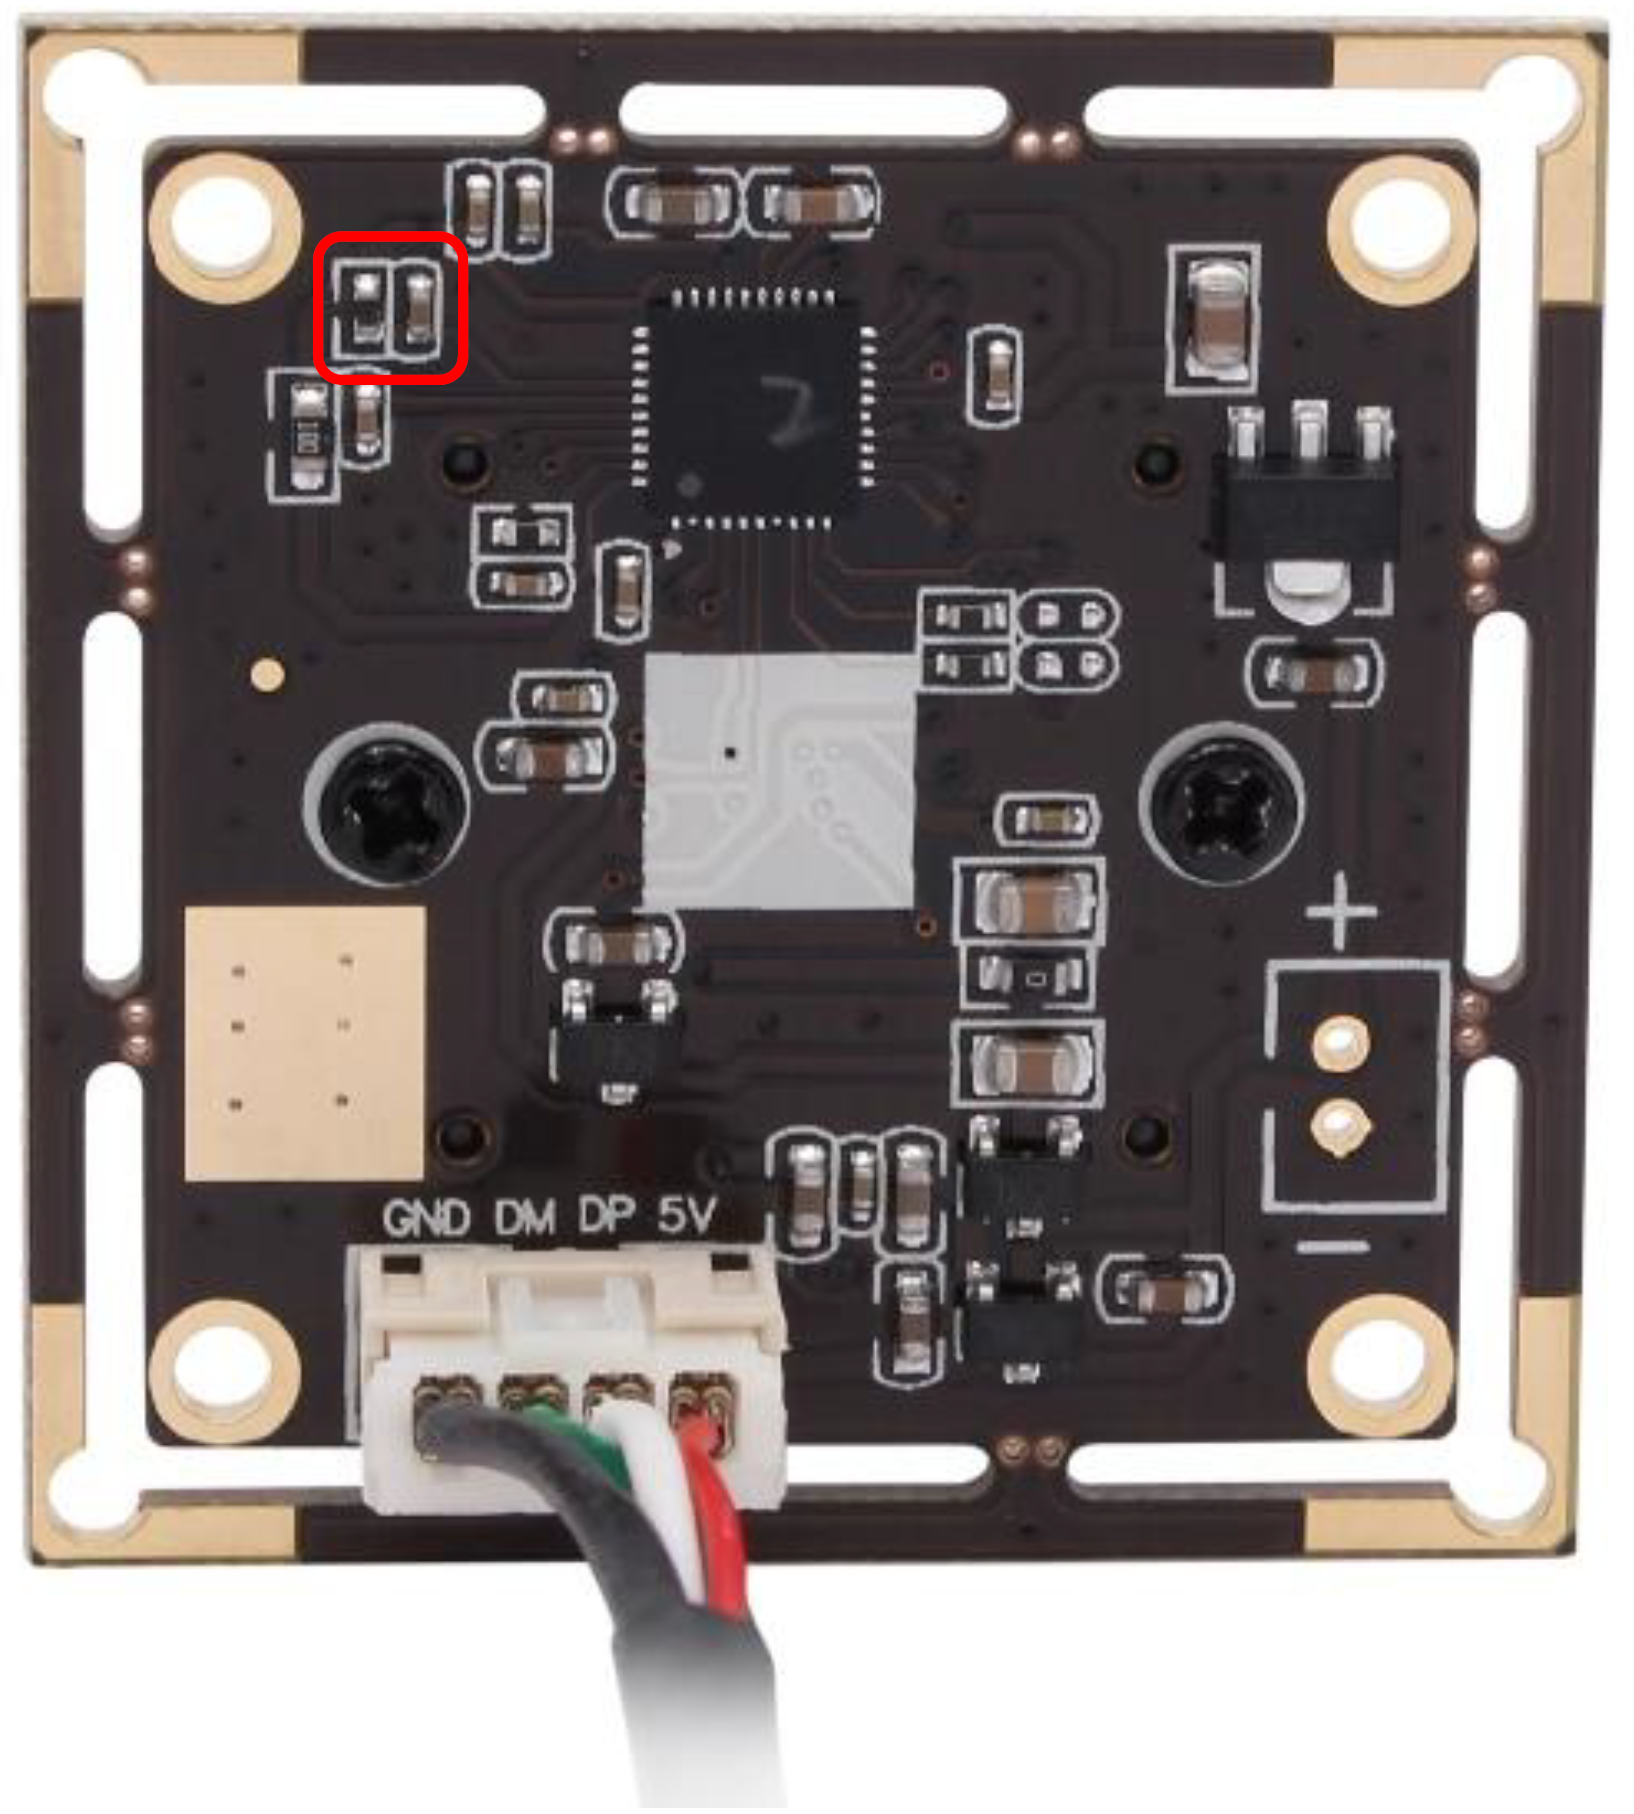
\includegraphics[height=5.5cm]{images/4_Design/Hardware/Camera-Modification.PNG}}}
    \caption{Camera Modification}
    \label{fig:camera-modification}
\end{figure}


\subsubsection{Temperature Sensor}
There are two temperature sensors embedded on the \acrshort{pcb}. One to measure the ambient temperature (and therefore be able to calculate the speed of sound in air according to the temperature, described in \ref{equ:speed_of_sound}) and the second-one to measure the system temperature which is used to control the speed of the four \acrshort{dc}-Fans. The temperature sensors used in the design are of the type \textit{TMP112} made by Texas Instruments. They have an accuracy of ±0.5\,°C and are connected to the \acrshort{i2c}-Bus of the system with individual IDs (\codeword{0x48} \& \codeword{0x49}). The temperature gets read every 500\,ms.

\subsubsection{Time-of-Flight Sensor}
For various safety reasons it is important to turn off the speaker output when a person enters the near-field of the Audio-Beamformer (d $<$ 1\,m). This safety mechanism has been realized by using a multi-zone \acrfull{tof} sensor. The \textit{VL53L5CX}, made by ST Microelectronics is specially designed for a wide field of view (63°). It can measure distances up to 4\,m and has a resolution of 8\,x\,8 zones. It is connected to the \acrshort{i2c}-Bus and can be address by the ID of \codeword{0x52}. The internal update rate has been set to 5\,Hz to minimize traffic on the \acrshort{i2c}-Bus. To further increase the data throughput, the \acrshort{i2c} clock rate has been set to 1\,MHz.

The distance-map data then gets further processed as described in section \ref{4_Sensors_Near-field}.

\newpage
\subsubsection{Rotary Encoder}
To easily adjust the volume of the Audio-Beamformer, a pushable rotary encoder has been placed below the display. Pressing the knob toggles the mute state of the output stage. This becomes very handy if the volume level should stay the same, but the speaker needs to be turned off temporarily. Both, the volume level and the mute state can be overwritten in the \acrshort{gui}. This is can only be achieved by the relative position measurement of rotary encoders and would not be possible with ordinary potentiometers.

To suppress contact bouncing and thus prevent false inputs, a simple RC debouncing circuit with a schmitt-trigger buffer has been installed.

\begin{figure}[h!]
	\centering
	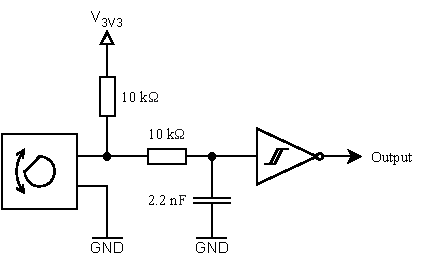
\includegraphics[width=8.5cm]{images/4_Design/Hardware/Rotary Encoder Debounce.pdf}
	\vspace{-0.1cm}
    \caption{Rotary Encoder Debounce-Circuit}
    \label{fig:rotary_encoder-debounce_circuit}
\end{figure}

\subsubsection{Power-Button and Cooling-Fans}
On the right side of the Audio-Beamformer, a 22\,mm stainless steel push button has been installed to power-on and off the Raspberry Pi Compute Module 4. The integrated \acrshort{rgb}-\acrshort{led} ring is driven by a specialized \acrshort{pwm}-Driver \acrshort{ic} with \acrshort{i2c}-Interface. The \textit{PCA9633DP1}, made by Texas Instruments provides four individual addressable 8-Bit \acrshort{pwm} channels and is addresses at the \acrshort{i2c}-Address of \codeword{0x62}. \acrshort{pwm}-Channel 1, 2 and 3 are used for the red, green and blue \acrshort{led}s of the bush button, while channel 0 is connected to the four \acrshort{dc}-Fans installed in the back of the enclosure. The Fans are wired in parallel and operate at a maximal voltage of 12\,V.\\
The system temperature is used to control the speed of the cooling fans. They start running at a temperature of 40\,°C and provide proportional air flow as the temperature increases. At 60\,°C the operate at full speed.

\subsubsection{LCD Touchscreen}
Since the beginning of the project, the idea was to create an attractive and modern looking device. One of the key components is the large \acrshort{lcd} touchscreen. It has a diagonal size of 11.9\,inch and a resolution of 1480\,x\,320 pixels. As interface, \acrshort{hdmi} is used for the video stream and \acrshort{usb} to transmit the touch-screen data to the Raspberry Pi Compute Module 4. Important to notice is, that the corners of the display are rounded (radius of 5\,mm), this has been considered when designing the \acrlong{ui}.

\subsubsection{RGB-LEDs}
To present a visual feedback of the current beam-steering angle and the active window-function, each row of the array contains one individually addressable \acrshort{rgb}-\acrshort{led} on top and on the bottom of the ultrasonic transducers. The type of those intelligent \acrshort{led}s is called \textit{APA102}. They embed an integrated driver \acrshort{ic} which can be controlled via a non-standard \acrshort{spi} protocol (special start and end sequence instead of a chip select line) in a daisy-chain configuration. The LEDs have a physical size of 5.0\,x\,5.0\,mm and are directly powered by the 5\,V voltage rail.\\
Next to the 38 \acrshort{led}s used for the array channel illumination, further 20 \acrshort{led}s are placed on a ring around the camera. This offers direct visual insight of the face-tracking algorithm. While a person is tracked, the \acrshort{led}s are animated in a "breathing" brightness motion. When there is no face detected, a spinning gradient animation is shown.\\
The maximal power consumption is about 25\,W if all \acrshort{led}s are fully turned on.

\subsubsection{External Interfaces}
The Audio-Beamformer can easily be connected to an external display by using the \acrshort{hdmi}-Port on the left side of the enclosure. In combination with the two spare \acrshort{usb}-Ports, e.g. for connecting a keyboard and mouse, the system can easily be debugged. Even developing new software features directly on the target platform is possible. To back-up the data of the \acrshort{emmc} flash storage on the Raspberry Pi Compute Module 4, a  \acrshort{usb} Type-C Port has been added. To start the back-up procedure, the tiny slide switch next to the \acrshort{usb}-C Port must be set to the up-position. This enables the bootloader of the Raspberry Pi Compute Module 4 on power-up of the device. When connected to an external host (such as a computer), the Audio-Beamformer gets recognized as a mass-storage-device. A back-up tool like e.g. \textit{Win32DiskImager} can be used to create a binary image of the operating system inclusive all user data.

\subsection{Output Stage}
The output stage represents a Class-D design in a \acrshort{mosfet} full-bridge configuration. This topology has the advantage of high efficiency and low part count. However, the proper design of such output amplifiers has its difficulties. Specially when operated at high switching frequencies (3.125\,MHz in this case), transient turn-on and turn-off times must be very short. This can lead to ringing and voltage spikes on the output signal.
\acrshort{mosfet}s are known to be very sensitive when it comes to such transient voltage spikes. Exceeding the maximal Drain-Source voltage will likely result in a breakdown and a permanent short circuit. To prevent such behavior, several options can be considered:

\begin{itemize}
    \item Utilize \acrshort{mosfet}s with higher voltage rating
    \item Reduce switching speed and therefore increase transient time
    \item Impedance matching of load and driving source (e.g. with series resistor)
    \item Introducing passive dampening networks, such as RC-Snubber circuits
    \item Dump excess energy into bypass capacitors using clamping diodes
\end{itemize}
\newpage

\acrshort{mosfet}s with higher Drain-Source voltage ratings have typically more gate capacitance and therefore would lead to a drastically higher switching current. A great compromise has been found with the type \textit{BSS123}, it has a Drain-Source voltage rating of 100\,V and can withstand a continuous current of 200\,mA. The gate capacity is around 32\,pF (at a gate voltage of 12\,V). 

\begin{figure}[h!]
	\centering
	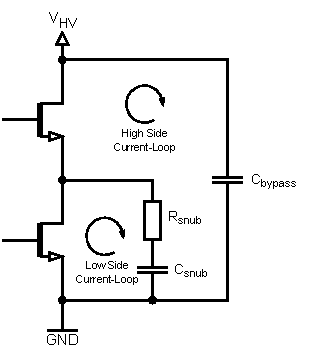
\includegraphics[width=5.5cm]{images/4_Design/Hardware/Class D Snubber.pdf}
	\vspace{-0.2cm}
    \caption{Class-D Half-Bridge with RC-Snubber}
    \label{fig:rc-snubber}
\end{figure}

As mentioned above, RC-Snubber networks can help to suppress voltage spikes by creating a low-impedance path for the current, circling in the low-side of the half-bridge. Figure \ref{fig:rc-snubber} shows how important a sufficient bypass capacitor is to stabilize the high-side. Texas Instruments published a very comprehensive guide on how to design such RC-Snubber networks \cite{ti_class_d_snubber_design}.

The amplified digitally modulated output signal must be low-pass filtered in order to suppress the high frequency switching content. This can easily be achieved by the use of a series inductance. To keep the design symmetrical, on both half-bridge output signals a shielded inductor with an inductance of 220\,$\mu$H has been installed. The inductance value has experimentally be evaluated by trying out different combinations of inductors and switch frequencies compared to the output noise level.
%\pagebreak

\subsection{Ultrasonic-Transducer Array}
Achieving a decent array size is important to get a better directivity, higher output volume and in general greater beam-steering properties. Thus a large amount of ultrasonic transducers is needed. In order to keep the cost down of the project, one of the key criteria was the unit price. Directly ordering by professional suppliers, such as Digikey, Mouser, Farnell, etc. results in very high prices of more than 7\,CHF per piece. This was not acceptable since more than 150 pieces are needed in the final design. Fortunately it was possible to get directly in touch with a manufacturer based in China. The datasheet of the \textit{MA40A16} (attached in the appendix \ref{appendix_ma401a6}) has been studied firmly, with the conclusion that the type is suitable for this project and satisfies all key parameters. The price per unit is only 0.3\,CHF.\\
They operate at a resonant frequency of 40\,kHz and have physical diameter of 16\,mm. Important to notice is, that the metal case makes electrical contact to one of the pins. Thus it's important to leave enough clearance between the transducers to prevent short circuits.

\subsubsection{Arrangement \& Placement}
As prior analysis showed, the denser an array can be built, the better is it's performance. Due to the circular shape of the ultrasonic transducers, the optimal arrangement is a hexagonal pattern. This has some further advantage of creating a smaller horizontal spacing between each row of ca. 14.75\,mm (when a diagonal distance of 17.0\,mm is chosen with a gab of 1\, mm between the transducers). In general, a smaller spacing leads to higher efficiency and a better beam pattern (e.g. less dominant side lobes).\\
The final number of 19 rows has been the result of several considerations. First of all, the row count must be odd, to create a symmetrical design with only one centre row. Further the total width of the array must comply with the maximal manufacturing and assembly size of \acrshort{pcb}s by JLCPCB (max. 480\,x\,320\,mm). And at last, the overall dimension should match the size of the display to create a cleaner visual impression of the final design. At some point, adding more rows to the array will not lead to any further audible improvements. This is mainly caused by the window-function which tends to strongly reduce the gains of the rows at both ends of the array.\\
A row height of 8 has been chosen to create stronger beam-characteristics, specially in the vertical direction. In addition, the parallel wiring of multiple ultrasonic transducers lowers the total impedance, which has the advantage of operating at a lower driving voltage to create the same amount of power.

\bigskip
\begin{figure}[h!]
	\centering
	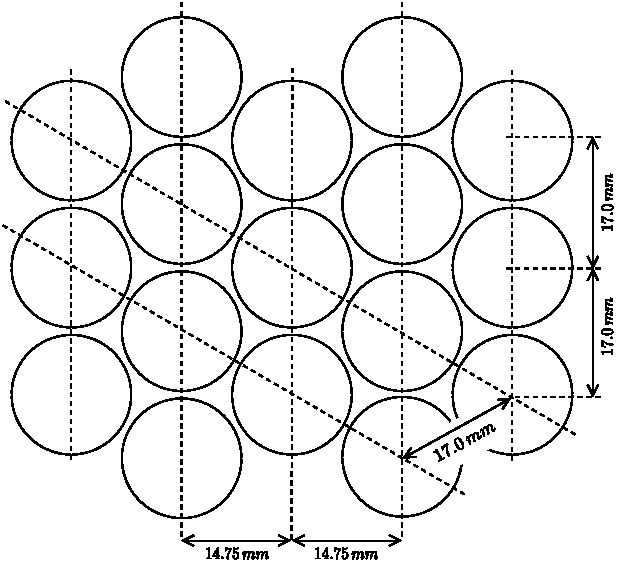
\includegraphics[width=10.5cm]{images/4_Design/Hardware/Transducer Placement.pdf}
	\vspace{0.2cm}
    \caption{Ultrasonic Transducer Placement}
    \label{fig:transducer-placement}
\end{figure}
\newpage

\section{FPGA Design}
As mentioned in Section \ref{hardware_fpga}, the \textit{Alchitry Cu} \acrshort{fpga}-Board has been used. The specific chip is called \textit{iCE40-HX8K}, made by Lattice Semiconductor. It offers a total of 7680 logic cells, 32 blocks of dual-port \acrshort{ram} (4\,KBit each), two independent \acrshort{pll}s and 79 \acrshort{io}-Pins. It is operated at 100\,MHz which is more than enough for this application.

\begin{figure}[h!]
	\centering
	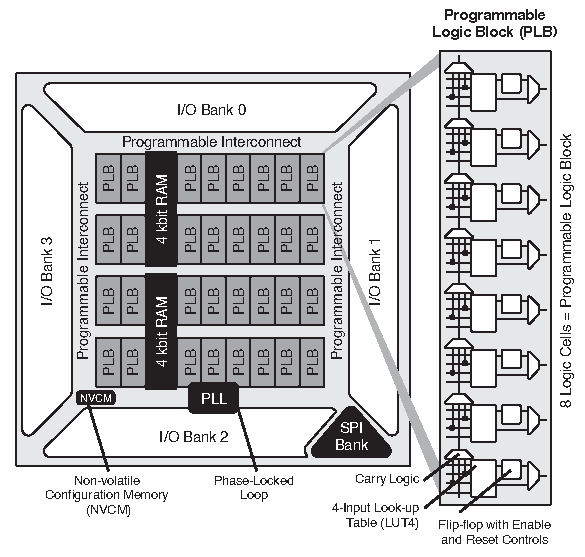
\includegraphics[width=9.5cm]{images/4_Design/FPGA/iCE40LPHXFamilyDataSheet.pdf}
	\vspace{0.0cm}
    \caption{Lattice iCE40 \acrshort{fpga} Family Architecture \cite{lattice_ice40_fpga_architecture}}
    \label{fig:rc-snubber}
\end{figure}

To keep the design process as efficient as possible, a development environment has been chosen which is easy to use and offers lots of predesigned \acrshort{ip}-Blocks. Namely the \mbox{\textit{IceStudio}} has been used in combination with the open source tool-chain called \textit{IceStorm} which currently supports all \acrshort{fpga}s of the iCE40-Family.\\
The tool offers a combination of a graphical design work-flow with the option of embedding custom blocks of Verilog code. Due to the open source nature, lots of individuals published extension libraries containing hundreds of \acrshort{ip}-Blocks. This becomes very handy, specially for integer arithmetic operations, such as addition and multiplication.

\subsection{Integer Arithmetic}
Signed integers with a fixed width of 16 bits have been chosen as a datatype. This has the advantage of making use of dedicated hardware accelerators built into the \acrshort{fpga}. The maximum range of a 16 bit integer reaches from -32,768 to +32,767. In order to make calculations easier, this range can be interpreted as normalized values between -1.0 (representing -32,767) and +1.0 (representing +32.767). Note that the most negative value of -32,768 should never be used, as the same positive value can't be reached (preventing asymmetric behaviour).\\
Using normalized values simplifies particularly the multiplication operation, since signals can be attenuated or mixed without the risk of a sign flip or the values getting clipped.
\newpage

\subsection{Signal Flow Diagram}
\enlargethispage{2.6cm}
\begin{figure}[h!]
	\centering
	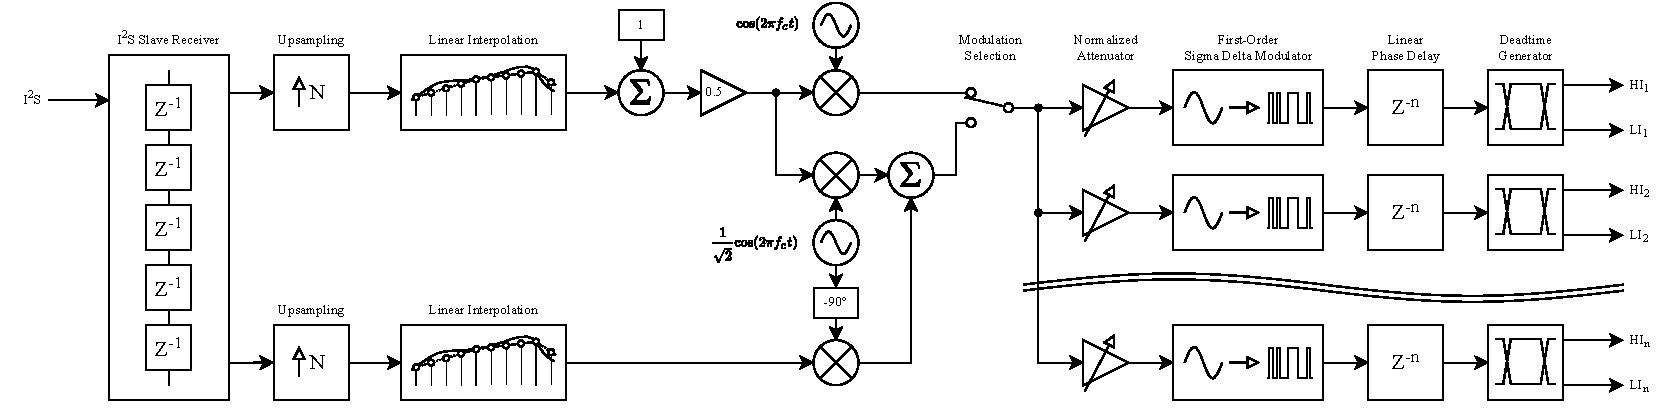
\includegraphics[width=22.7cm, angle=90]{images/4_Design/FPGA/FPGA Block Diagram.pdf}
	\vspace{-0.2cm}
    \caption{FPGA Signal Flow Diagram}
    \label{fig:fpga-signal-flow}
\end{figure}

\newpage
\subsection{Clock \& Synchronization}
Making sure that both \acrshort{fpga}s run simultaneously and don't drift apart in time, the system clocks must be shared. This means that one of the \acrshort{fpga}s acts as a master, which provides a clock signal to all slaves. In order to use the same logic configuration, a dedicated ID-Pin has been added to differentiate the master (logic level 0) and the slave (logic level 1).\\
The clock is initially created by an 100\,MHz oscillator built onto the development board. With the help of a \acrshort{pll} it can be adjusted to the needs of the application. However, in this case it turned out to be a well functioning core speed and no further adjustments have been done. If a reduction of power consumption is needed, the clock speed could be decreased.

In addition, a synchronization pulse gets created by the Raspberry Pi Compute Module 4 at the startup of the device. This signal is used to reset the local oscillators on all \acrshort{fpga}s, to make sure that the phase of the carrier signal is in sync.

\subsection{I\textsuperscript{2}S Interface} \label{fpga_i2s}
The \acrshort{i2s}-Interface is a well known and widely used protocol for real time digital audio streaming. It is mainly used for inter-chip communication (therefore its name of \acrlong{i2s}). The interface consists of 3 signals: BCLK or just BCK (Bit Clock), LRCLK (Left-Right Clock) and the unidirectional data signal. The LRCLK is used for frame synchronization and indicates the current channel that is being transmitted (logic level 0 means left channel). The start of a frame is defined by the falling edge of the LRCLK signal. On the rising edge of the BCK signal, the current data bit gets transmitted and fetched.\\
There exist various frame lengths, but the most common is 24 bit per channel, in a "left-aligned" manner. The default \acrshort{i2s} configuration of the Raspberry Pi Compute Module 4 has been implemented on the \acrshort{fpga}. This means a sample rate of 44'100\,kHz has been used. However, only the upper 16 bits of the 24 bit audio-stream get utilized for further processing, since a higher dynamic range is not needed. This has the advantage of simplifying the processing due to the use of fixed 16 bit integer arithmetic operations.

The implementation in the \acrshort{fpga} is straight forward. Basically a chain of D-Flip-Flops is created where the data is fed through. On the falling edge of the LRCLK signal, the data is then fetched and ready to be processed.

\todo[inline]{Include Graphic}

\newpage
\subsection{SPI Interface} \label{fpga_spi}
The \acrfull{spi} is used for controlling the configuration of the \acrshort{fpga}s. The protocol is very simple and can easily be implemented as a chain of shift registers (consisting of cascaded D-Flip-Flops). This structure allows daisy-chain operation, where the output of the first \acrshort{fpga} is fed into the input of the second one. The interface consists of 3 signals: CS (Chip select), SCLK or just SCK (Serial Clock) and the data signal, often called MOSI (Master-Out $\rightarrow$ Slave-In). The data gets shifted through the shift registers at each rising edge of the clock signal by one position. At the rising edge of the chip select signal, the current state then gets fetched from the shift-register chain to the output. \\
A clock frequency of 8\,MHz has been chosen to ensure fast update rates. In Table \ref{tab:spi_protocol} the protocol gets described further.


\begin{table}[h]
    \hfuzz=23.0pt
    \begin{tabular}{ | p{2.8cm} | p{3.0cm} | p{6.6cm} |}
      \hline
      \multicolumn{1}{|c|}{\textbf{Byte Number}} & \multicolumn{1}{c|}{\textbf{Data Type}} & \multicolumn{1}{c|}{\textbf{Description}}\\ \hline
      \codeword{[0]} & binary & \codeword{[2:0]} Interpolation: 1 ... 64 \\
                   &        & \codeword{[3]  } Modulation Type: AM / MAM \\
                   &        & \codeword{[7:4]} Reserved \\ \hline
      \codeword{[2:1]} & boolean & \codeword{[9:0]} Channel Enable (0 ... 9)\\ \hline
      \codeword{[4:3]} & unsigned integer & Sigma-Delta Coefficient \\ \hline
      \codeword{[6:5]} & unsigned integer & Channel 0 Delay \\ \hline
      \codeword{[8:7]} & signed integer & Channel 0 Gain  \\ \hline
      \codeword{[10:9]} & unsigned integer & Channel 1 Delay \\ \hline
      \codeword{[12:11]} & signed integer & Channel 1 Gain  \\ \hline
      ... & ... & ...  \\ \hline
      \codeword{[38:37]} & unsigned integer & Channel 8 Delay \\ \hline
      \codeword{[40:39]} & signed integer & Channel 8 Gain  \\ \hline
      \codeword{[42:41]} & unsigned integer & Channel 9 Delay \\ \hline
      \codeword{[44:43]} & signed integer & Channel 9 Gain  \\ \hline
      \codeword{[45]} & binary & \textit{Same as above, Byte 0} \\ \hline
      \codeword{[47:46]} & boolean & \codeword{[9:0]} Channel Enable (19 ... 10)\\ \hline
      \codeword{[49:48]} & unsigned integer & Sigma-Delta Coefficient \\ \hline
      \codeword{[51:50]} & unsigned integer & Channel 10 Delay \\ \hline
      \codeword{[53:52]} & signed integer & Channel 10 Gain  \\ \hline
      \codeword{[55:54]} & unsigned integer & Channel 11 Delay \\ \hline
      \codeword{[57:56]} & signed integer & Channel 11 Gain  \\ \hline
      ... & ... & ...  \\ \hline
      \codeword{[83:82]} & unsigned integer & Channel 18 Delay \\ \hline
      \codeword{[85:84]} & signed integer & Channel 18 Gain  \\ \hline
      \codeword{[87:86]} & unsigned integer & Channel 19 Delay \\ \hline
      \codeword{[89:88]} & signed integer & Channel 19 Gain  \\ \hline
    \end{tabular}
    \caption{\label{tab:spi_protocol}SPI Protocol Description}
\end{table}

\todo[inline]{Include Graphic}

\newpage
\subsection{Interpolation} \label{fpga_interpolation}
To enhance the \acrfull{snr}, the incoming base band signal gets up-sampled to a sampling rate of 6.25\,MHz. Oversampling improves the \acrshort{snr} by the following factor:
\begin{equation}
    \Delta SNR \approx 0.5 \log_2 \left(\frac{6.25\,MHz}{44.1\,kHz}\right)\  6.02\,dB = 21.5\,dB
\end{equation}
The formula however implies, that the signal gets perfectly interpolated and reconstructed. This is definitely not the case if simple sample-and-hold methods are applied. To improve the signal quality, linear interpolation is used. The implementation allows to change the interpolation depth between 1 (no interpolation) and a maximum of 64. However in practice, there is not really a noise reduction noticeable when the linear-interpolation gets enabled or the interpolation depth gets increased. The audible noise is mostly caused by other factors, such as the sigma-delta-modulator, clock jitter, phase noise, etc.

\subsection{Modulation}
There are two modulation types implemented: Regular amplitude modulation and modified amplitude modulation (similar to \acrlong{qam}). Both modulation types are build around a mixer (multiplier), which multiplies the base band signal with the carrier oscillator, in this case a 40\,kHz sine wave. This sinusoidal signal gets created by a \acrfull{lut} which is stored in Block-\acrshort{ram}. The table is automatically generated by a Python script.\\
Important to note is that there are two different \acrshort{lut}s for each modulation type. The values for the regular amplitude modulation are fully scaled and calculated like this: $f_{AM}(t) = \cos(2\pi f_c t)$, where for the modified amplitude modulation a reduced amplitude is used of the factor: $1/\sqrt{2}$.

This prevents the case, where a value of more than ±1 occurs and could cause an arithmetic overflow
\begin{equation}
    f_{MAM}(t) = Q(t)\frac{1}{\sqrt{2}}\cos(2\pi f_c t) + I(t)\frac{1}{\sqrt{2}}\cos(2\pi f_c t - \frac{\pi}{2})  \overset{!}{\leq} 1.
\end{equation}

\subsection{Sigma-Delta-Modulator}
In order to keep the overall complexity as low as possible, the focus has been set onto the implementation of a first-order sigma-delta modulator. Higher order sigma-delta modulators tend to have better noise-shaping capabilities and thus will result in a lower \acrshort{snr}. The implementation complexity however, increases drastically with higher orders, as e.g. specially tuned \acrshort{iir}-Filters are needed.

The first-order implementation is very straight forward. The core consists of an integrator (binary adder) and a feedback-loop constructed with a single D-Flip-Flop stage. Basically the output of the integrator tries to "follow" the input signal, similar to any control loop. The error (difference between the target and actual value) is the source of the modulating output signal. The \acrshort{msb} (sign bit) is used to determine if the error is positive or negative. This binary output single tends to toggle at a very high frequency (up to half the sigma-delta clock rate). The spectral view shows a clearly shifted noise level to the higher frequency range. When the output signal gets low-pass filtered (by a physical analog filter), the switching noise gets suppressed and the main low-frequency target signal shows up with a much higher \acrshort{snr}.

The steepness of the integrator can be adjusted by the "addition-factor". This coefficient has major impact on the spectral noise figure. It turned out to be rather complex to find an optimal value, the implementation allows to adjust the coefficient by software over the \acrshort{spi}-Interface. Extensive tests showed that in combination with the chosen analog filter (inductance value), a sigma-delta-modulator coefficient of 8,192 performs best.

As described in Section \ref{fpga_interpolation}, the higher the over-sampling ratio, the greater the \acrshort{snr}. Increasing the clock rate has however the major disadvantage of creating much more switching losses. A clock frequency of 6.25\,MHz has proved to be sufficient for both, low audible noise and reasonable switching losses. This results in a output bandwith of $B=3.125$\,MHz.

\begin{figure}[h!]
    \centering
    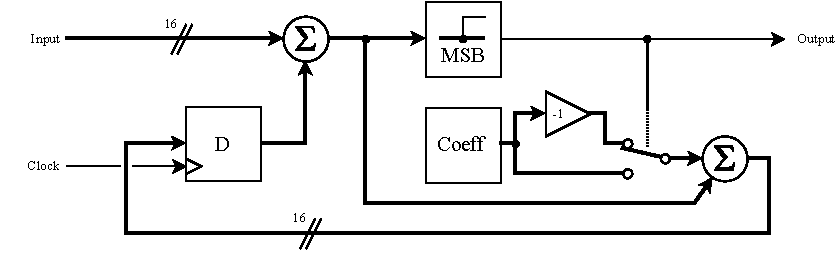
\includegraphics[width=\textwidth]{images/4_Design/FPGA/Sigma-Delta-Modulator.pdf}
    \caption{First-Order Sigma-Delta-Modulator}
    \label{4_fig:fpga_Sigma-delta-modulator}
\end{figure}

\subsection{Channel Delay \& Gain}
Each channel can be attenuated and delayed individually. The gain-factor can ether be positive or negative, which can be used to flip the phase polarity to 180°. This is needed for some window-functions. Note that for normal operation (no attenuation) a gain-factor of 1.0 (integer value of +32,767) must be set.

The delay line has been implemented as a ring buffer structure in Block-\acrshort{ram}. The dual port configuration is needed, since data is getting written and read at the same time at different memory addresses. The signal flow diagram \ref{fig:fpga-signal-flow} shows that the delay-line block has been placed at the far end of the processing pipe-line. This means, only a single bit (namely the binary output signal of the sigma-delta-modulator) must be stored instead of a 16 bit integer vector.\\
Due to the maximal capacity of 4\,kBit per \acrshort{ram}-Block, the signal can be delayed by a maximum of 4,092 ticks. However the configuration of those \acrshort{ram}-Blocks allows only a minimum bus-width of 2 bits.This means that one memory cell must be filled with two single-bit samples. As a result, the signal can be delayed in 2,047 adjustable steps (0 ... 2,046). The tick time is derived by the Sigma-Delta-Modulator frequency, in this case: \mbox{$\Delta t = 1/6.25$\,MHz$ = 160$\,ns}. This results in a maximal delay time of \mbox{$t_{max} = 4092\ \Delta t \ \approx \ 654.7\,$ns}. In Section \ref{beamsteering_delays} the calculation of the delay time, based on the beam-steering angle, is further described.

\todo[inline]{Include graphic of ring buffer structure}

\subsection{Dead Time Generator}
The \acrshort{fpga} directly drives the high and low side of the Class-D output stage. In any half-bridge design it is key to make sure that at no time, both the high-side and low-side \acrshort{mosfet}s are turned on at the same time. Violating this restriction, causes a temporary short circuit when switching. This can lead to inefficiency and must be prevented in any case. The solution is very simple. Adding a fixed delay before turning on any \acrshort{mosfet} makes sure, that the complementary side is for sure not conductive anymore. This time is called "dead-time".

In the \acrshort{fpga} a dedicated dead-time-block has been implemented to create the exact timings for this particular hardware configuration. A dead time of 50\,ns has been chosen as a good trade-off since it leaves enough timing margins, but also ensures high efficiency. If the dead time is set to high, the output power will decrease significantly. In addition the \acrshort{snr} will become smaller and harmonic distortion will become noticeable.

The dead time generator block also provides a possibility to shut down the output completely. This can be handy for debugging purposes or to show the effect of a smaller array. The channel enable function is configurable per \acrshort{spi}-Interface.

\todo[inline]{Include Graphic}

\newpage
\section{Software Design}
The software on the Raspberry Pi was written in Python 3.9.2 due to its simplicity. However,  most libraries in Python being implemented in the background with C it is still fast enough for real-time audio processing.
The program was also built so that it can be run on Windows or Linux and not have a necessity for the hardware to be there.
\subsection{Structure}
The software structure of the Audio-Beamformer program is shown in Figure \todo{Figure}. The AudioBeamformer module creates all the instances of the other modules and distributes them accordingly to the submodules. Each module has for the initialisation a begin function and for correctly destructing it a end function. 

\todo[inline]{Include Graphic}

\newpage
\subsection{GUI}
The GUI was made with PyQt, a wrapper for Qt in python. The main goal was to create an intuitive, easy-to-use, and informative graphical user interface. 
The three main sections of the UI can be reached through the buttons on the left. We separated the configurable parameters into three sections, processing, channels, and settings. General settings such as mute, volume, and output level are always present on the right side of the screen. 
\subsubsection{Processing}
The processing window is divided into five different sections. All of these sections contain settings for audio processing.
\begin{enumerate}
    \item Source \\
    The audio input source and gain can be adjusted in this section. A gauge was added to get direct visual feedback on the input sound level.
    \item Equalizer \\
     In the second section, the equalizer can be enabled and chosen from the preset list. A bode plot can be seen at the bottom to give more information about the current equalizer used. 
    \item Interpolation \\
    In this section, the interpolation can be enabled, and the oversampling rate can be chosen. The oversampling values are 2, 4, 8, 16, 32, and 64.
    \item Modulation type \\
    In the last section the modulation type can be chosen. Additionally if the modulation type chosen is MAM a gain for the distortion channel can be set. 
\end{enumerate}

\begin{figure}[h!]
    \centering
    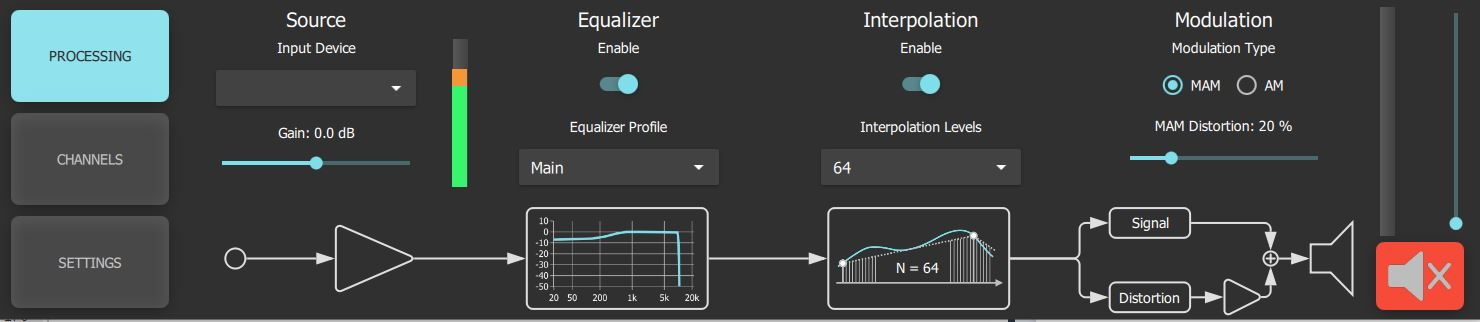
\includegraphics[width=\textwidth]{images/4_Design/GUI_Processing.JPG}
    \caption{GUI Processing View}
    \label{4_fig:gui_processing}
\end{figure}
\todo[inline]{Update Graphic}

\subsubsection{Channels}
The channels window is split up into 3 different areas.
\begin{enumerate}
    \item Beamsteering \\
    In this section, beamsteering can be enabled, and the angle source can be set. If the angle source is set to "Camera" the face tracking is activated, else if it is set to "Manual" a slider appears with which the angle can be set manually. The last angle source is "Pattern" for which a predefined pattern of angles are set for a predefined time. 
    \item Window \\
    In this section the window function can be enabled. If it is disabled the window "Rectangle" is used. To give more information about the current window function, a plot of how the gains are set is shown at the bottom.
    \item Video feed \\
    In this video feed one can see who is currently being detected and tracked. If a light blue window surrounds a face this is the current tracked face. If it is grayed out a face was detected but is currently not tracked.
\end{enumerate}
\begin{figure}[h!]
    \centering
    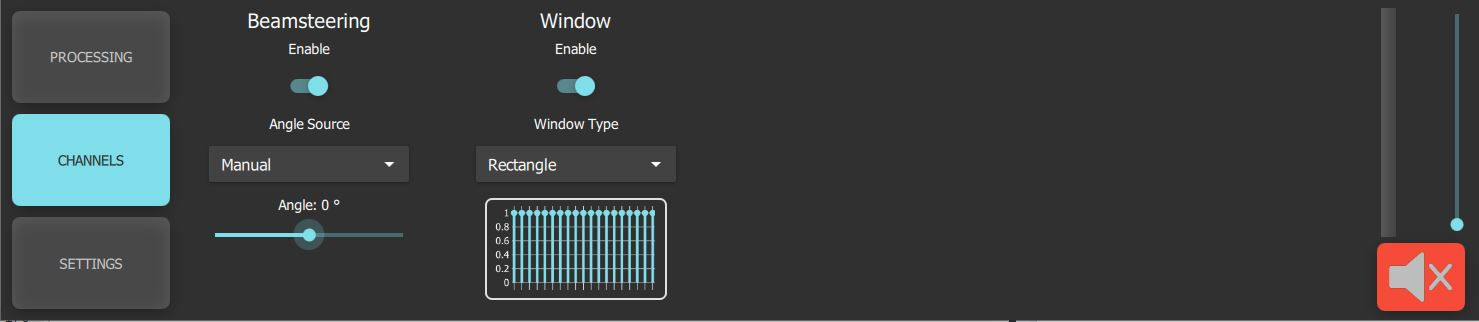
\includegraphics[width=\textwidth]{images/4_Design/GUI_Channels.JPG}
    \caption{GUI Channels View}
    \label{4_fig:gui_channels}
\end{figure}
\todo[inline]{Update Graphic}

\subsubsection{Settings}
The setting page is split up into 6 different areas.
\begin{enumerate}
    \item LED \\
    In this section the LEDS can be enabled and their brightness can be set. 
    \item ToF Sensor \\
    In this section the ToF Sensor can be disabled and its sensitivity can be changed. To get a visual feedback of the sensitivity a gauge is present.
    \item Max volume \\
    With this slider the maximum volume which can be reached by the loudspeaker can be adjusted. This can be done if the device needs to be used inside to guarantee safety.  
    \item Beamfocusing \\ 
    In this section the beamfocusing can be enabled and the distance where the beams should meet can be adjusted. 
    \item Stats
    This section shows temperature and load information about the system and the CPU.
\end{enumerate}
\begin{figure}[h!]
    \centering
    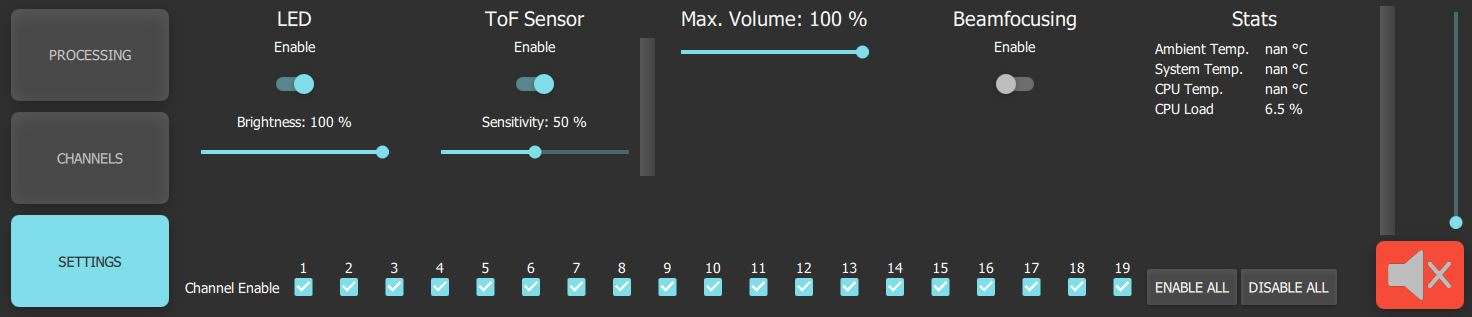
\includegraphics[width=\textwidth]{images/4_Design/GUI_Settings.JPG}
    \caption{GUI Settings View}
    \label{4_fig:gui_settings}
\end{figure}
\todo[inline]{Update Graphic}

\subsection{Audio Processing}
In this module the audio processing is made. First the audio input is read block based into the program then the audio is filtered through an equalizer and changed for the modulation and in the end it is outputted through \acrshort{i2s} to the \acrshort{fpga}.
\subsubsection{Audio Stream}
The audio stream is implemented in python using a library called "Sounddevice", which wires the input to the output in a non blocking way. The audio is read block based with a block size of 8192. We tried to keep the block size as small as possible to guarantee low latency if a microphone is used. 
\subsubsection{Equalizer}
To compensate the distortion generated by the frequency response of the transducer, which is shown in Section \ref{6_sec:Frequency_response}, a FIR equalizer can be enabled between the input and the output of the audio stream. New equalizers can be added easily into the code. 
\subsubsection{Modulation Type}
Currently the two modulation types implemented are \acrshort{am} and \acrshort{mam}.
The left channel carries always the processed audio information.
In the case of \acrshort{am} the right channel is just a copy of the left channel, but in case of \acrshort{mam} it is a second order approximation of the distortion term shown in Equation \ref{3_eq:mam_distortion_approx} 
\begin{equation}
    \text{Left Channel} = 1 - \frac{1}{2}i(t)^2 - \frac{1}{8}i(t)^4.
\end{equation}
Where $i(t)$ is the incoming audio signal. 
\subsection{Beam Steering}
In the beam-steering modules delay and gain for all the channels are calculated and are adjusted using the SPI-Interface. 
\subsubsection{Channel Delays} \label{beamsteering_delays}
The formula used for calculating the individual delays are
\begin{equation}
    \tau_m = m\frac{d}{c_0}\sin{\varphi},
\end{equation}
where d is the distance between the transducers, $\varphi$ the angle to steer to and $c_0$ the sound of speed. The sound of speed is also directly calculated in this module by using the ambient temperature input from the sensors module using the formula
\begin{equation}
    c_o = 331.5 + 0.607 \cdot T_{\text{Ambient}}
    \label{equ:speed_of_sound}
\end{equation}
The minimum angle which a phased array can reach is determined by the physical properties of the construction and by the smallest delay that can be applied to a signal. The physical properties of the transducer arrays are a spacing of $d=14.75 \,$mm and the numbers of channels $M=19$. The smallest delay in our case is $\tau_{min} = \frac{2}{6.25 \,\text{MHz}} = 320\,$ns and is determined by the output sampling rate
\begin{equation}
    \varphi_{min} = \arcsin{\left ( \frac{\tau_{min} c_0}{M d} \right ) } \approx  0.21^{\circ}.
\end{equation}
The maximal angle that can be reached is determined by the largest delay that can be applied to a signal. This is determined by the maximum number of memory cells, which in this case is $N_{MC} = 4092$, available for a channel on the FPGA. The largest delay that can be applied is $\tau_{max} = \tau_{min} \cdot N_{MC} \approx 654 \, \mu$s. Which leads to a maximal angle of 
\begin{equation}
    \varphi_{max} = \arcsin{\left ( \frac{\tau_{max} c_0}{M d} \right ) } \approx  53.4^{\circ}.
\end{equation}
\subsubsection{Channel Gains}
For controlling the main lobe with and side lobe level different windows can be applied to the loudspeaker. In addition to the gain of the channel this also effects the brightness of the LEDs to give the user more information about the window. 
\subsection{Sensors}
In the sensor module the different types of sensor of the Audio-Beamformer are read from submodules, processed and distributed. This is done in a way that other modules can easily access information from the sensors. 
\subsubsection{Near-Field Avoidance System} \label{4_Sensors_Near-field}
The \acrshort{tof} sensor gives a $8 \times 8$ matrix of distance values. To get from this an approximation for the distance where a person could be standing a simple thresholding is made, are any values below the distance where a person is allowed to stand? If yes then a two dimensional convolution is made with a $2 \times 3$ mask made out of ones is made. If now any value is bigger then a predefined threshold, done with the sensitivity, a person is detected.  

\subsection{Face Tracking}
To be able of directing the audio beam towards a specific person, a face-detection algorithm is needed. It is key to differentiate between multiple recognized faces. An additional restriction is the limited processing power of the Raspberry Pi Compute Module 4, since it does not have a dedicated \acrfull{gpu} or other hardware accelerators.

This part of the project has mostly been out-sourced, due to overall lower priority compared to other parts of this thesis. In particular, Luca Jost has developed the face-detection and tracking algorithms. The detection is based on a neural network called \acrshort{mnn}, more on that later \ref{software_mnn}.

In order to keep track of each individual person as people are moving around, a tracking algorithm has been implemented. To achieve this task, a Kalman-Filter has been used. After a certain amount of time, a newly detected face gets started to be tracked. This prevents rapid flickering of unwanted falsely detected faces (popping up on single frames). The algorithm keeps track of each face, even if the view gets interrupted for a short amount of time, e.g. the person tilts its head or moves behind an obstacle.

The FaceTracking module provides a chronologically sorted list containing the coordinates of each currently tracked face. The beam-steering module picks always the lowest index of this list, meaning the person who is tracked the longest amount of time. As soon as this person disappears on the frame, the list gets shifted to the left and the next person (now again oldest in list) is getting picked as a new target.

\subsubsection{Mobile Neural Network}\label{software_mnn}
To detect multiple faces on an image, deep learning learning techniques are applied. The \acrfull{mnn}, developed and trained by the Alibaba Group, offers advanced trained models and a highly efficient processing core, which is specially optimized for mobile devices with limited processing power. With the help of the python library called \mbox{\textit{PyTorch}}, machine learning algorithms can easily be applied on a high level abstraction layer and used with scripting languages like Python.

\subsection{Operating System}
The \acrfull{os} on the Raspberry Pi Compute Module 4 is called \textit{Raspberry Pi OS} and is based on Linux. It is key to use the 64 Bit version, since frameworks like \acrshort{mnn} and PyTorch cannot be run on a 32 Bit \acrshort{os}. In this project, the graphical \acrshort{os} version has been used, as it is more convenient to work with. The disadvantage is however, that the boot time is significantly longer (ca. 20\,s).

\subsubsection{Wireless Audio Streaming}
As input sources, Bluetooth$^{\circledR}$ audio streaming and AirPlay$^{\circledR}$ (product of Apple Inc.) are supported. This offers the very convenient possibility to stream music directly from any mobile device (such as smartphones or laptops) to the Audio-Beamformer. Important to note is that, for connecting via AirPlay$^{\circledR}$, both devices need to be in the same wireless network.

The wireless signal strength is attenuated by the metal enclosure. This leads to a smaller range of a reliable audio streaming transmission. Tests have shown that a distance of more than 3\,m can become problematic. This issue could be overcome by connecting an external antenna to the Raspberry Pi Compute Module 4.

\newpage
\section{Mechanical Design}
The mechanical design has proven to be a substantial part of the overall development process. With the help of modern \acrshort{cad} tools like \mbox{\textit{SolidWorks 2022}}, the design of the mechanical parts could vastly be accelerated.\\
A further advantage of creating an exact 1:1 model of the complete product is the possibility to render photo-realistic images or videos. They can be used as attractive illustrations or for advertising purposes. As a 3D rendering tool, \mbox{\textit{SolidWorks Visulize 2022}} has been used.

\subsection{Concept}
The mechanical concept of the Audio-Beamformer connects several considerations. First of all, acoustic constrains had to be discussed (e.g. avoiding vibrations of loosely connected parts). Next, the electrical part must comply with regularisation and common standards (e.g. safe to operate at mains voltage). Further, all mechanical parts should be easy to manufacture and assemble. This helps reducing the cost, makes the design more accessible and improves the overall service capability. At last, the complete assembly should have a professional and modern appearance. Combining all those factors resulted in a fully customized  and sturdy construction of an enclosure.

\bigskip
\begin{figure}[h!]
	\centering
	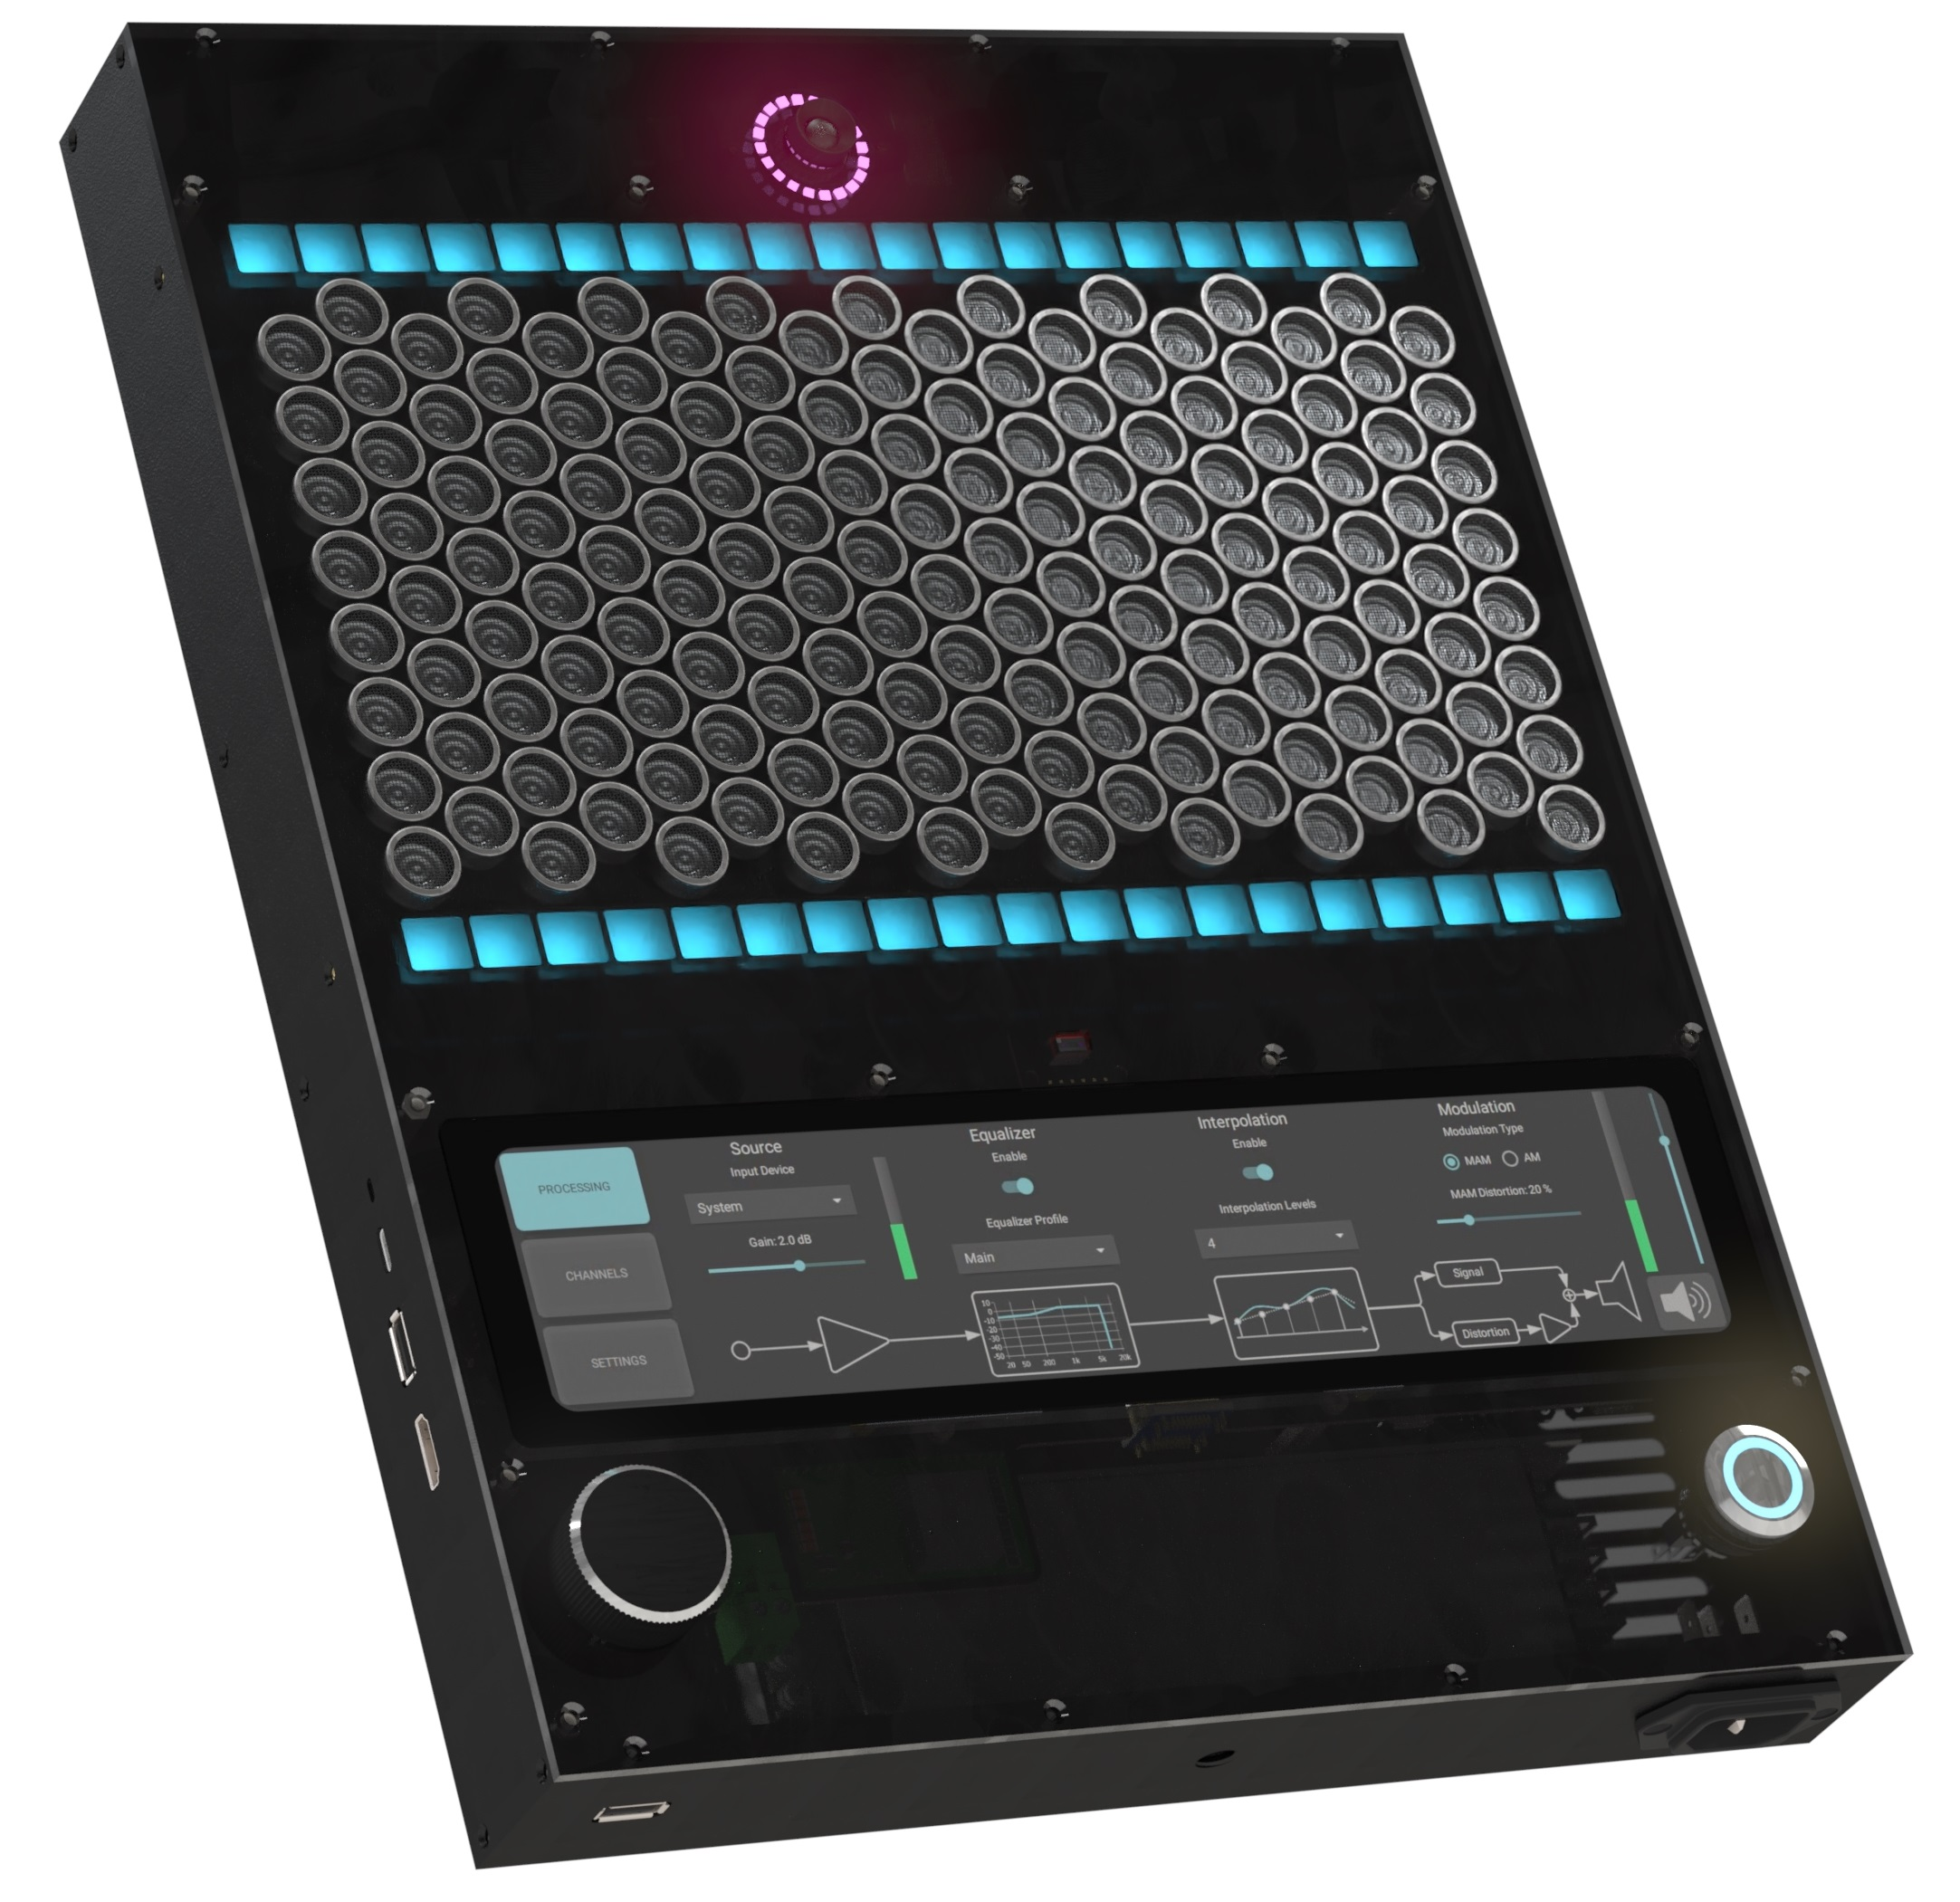
\includegraphics[width=13cm]{images/4_Design/Mechanical/Audio-Beamformer_Case.jpg}
	\vspace{0.0cm}
    \caption{3D-Render of final Product}
    \label{fig:final_product_render}
\end{figure}
\newpage

\subsection{Enclosure}
The case of the Audio-Beamformer is a combination of an aluminium sheet metal construction with a transparent acrylic front panel. The \acrshort{pcb} is held in place by M3 spacers from both the front and rear side ("sandwich" construction). The top and bottom plate is made out of 8\,mm thick aluminium bars. This is necessary, since they create a solid connection point to all other mechanical parts. The back and front panel have a thickness of 3\,mm and the side panels (left and right) of 1.5\,mm.

In the centre of the base plate, a $3/8\,"$ thread (DIN 4503-1 / ISO 1222) has been cut. This provides the possibility of attaching the Audio-Beamformer onto any standard camera tripod. Care has been taken that the fixture is capable of carrying the total weight of the Audio-Beamformer.

All aluminium sheet metal parts, as well as the acrylic front panel, have been laser-cut. All other components have been manufactured by conventional methods in the workshop at the university of \acrshort{ost}.

the final dimensions of the Audio-Beamformer are: 304\,x\,393\,x\,46\,mm. The total weight is: 3.88\,kg.



\chapter{Risks \& Safety}
\section{Risks}
The maximum sound pressure level that is allowed by \acrshort{suva} is $140 \,$dB and the averaging level 8h/day has to be below $110 \,$dB.The averaging level $L_m$ is given as
\begin{equation}\label{5_Safety_eq:AveragingLevel}
    L_m = 10 \log_{10} \left (  \frac{1}{T} \int_0^T 10^{0.1 L_p(t)}dt\right ).
\end{equation}
This can be solved for the sound pressure level $L_p(t) = L_p$ if it is assumed to be constant over a certain time $\tau$.
\begin{equation}\label{5_Safety_eq:AveragingLevel_SPL}
    L_p = L_m - 10\log_{10}\left ( \frac{\tau}{8} \right )
\end{equation}
To calculate the sound pressure level at any given point the directivity of the used transducers has to be calculated. As explained in Section \ref{3_sec:directivity} the sound directivity can be calculated as
\begin{equation}\label{5_Safety_eq:Directivity}
    Q_D = \frac{2 p(0)^2}{\int_{0}^{\pi}p^2(\theta)\sin{\theta}d\theta}. 
\end{equation}
The sound pressure ratio emitted by the transducers according to the data sheet is displayed in \ref{5_fig:directivity_transducer}.
\begin{figure}
    \centering
    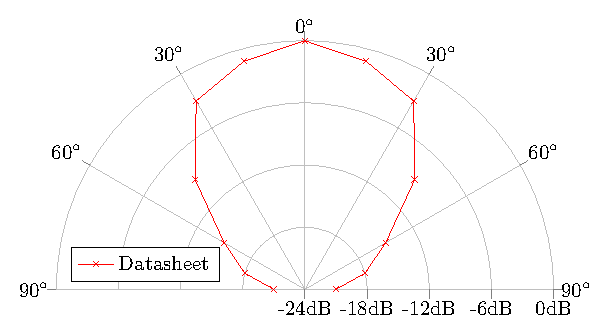
\includegraphics[width=0.8\textwidth]{images/5_Safety_Risks/Polar_PlotDirectivity.pdf}
    \caption{Directivity of a transducer}
    \label{5_fig:directivity_transducer}
\end{figure}
With this information the directivity index turns out to be $Q_D = 22$ with which the maximum sound power level in relation to the distance of the listener can be calculated as
\begin{equation}
         L_{wmax} 
     = 
     \underbrace{L_{pmax}}_{140dB} - 10\left ( \underbrace{\log_{10}(Q_D)}_{1.35B} - \log_{10}(r^2) - \underbrace{\log_{10}(4\pi)}_{\approx 1.1B}  \right ) = 137.5 + 20\log_{10}(r).
\end{equation}
The maximum sound power allowed in relation to the distance is plotted in Figure \ref{5_Safety_fig:Max_power_allowed}.
\begin{figure}
    \begin{minipage}{0.49\textwidth}
        \centering
        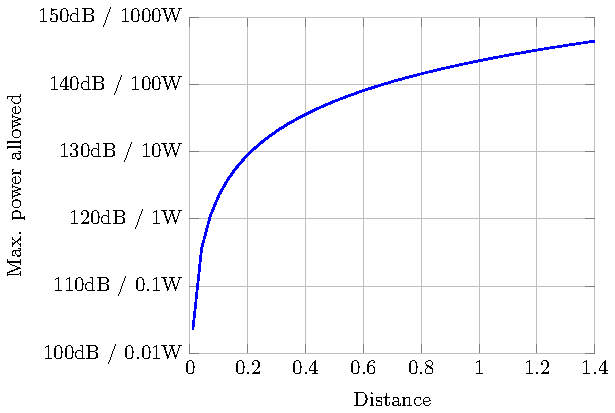
\includegraphics[width=\textwidth]{images/5_Safety_Risks/Max_Power_Allowed.pdf}
        \caption{Maximum sound power allowed}
        \label{5_Safety_fig:Max_power_allowed}
        \end{minipage}
    \begin{minipage}{0.49\textwidth}
        \centering
        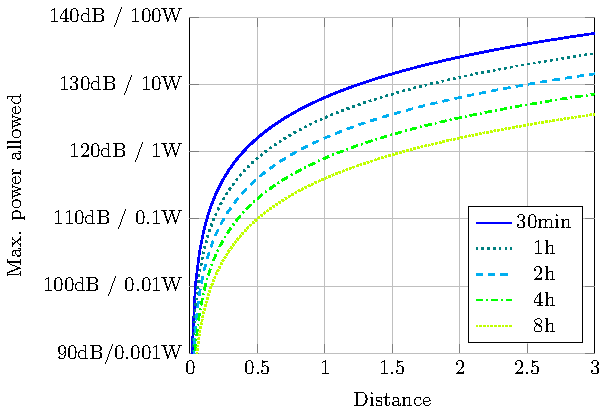
\includegraphics[width=\textwidth]{images/5_Safety_Risks/Max_Power_Allowed_Time.pdf}
        \caption{Maximum power allowed over time daily}
        \label{5_Safety_fig:Max_power_allowed:daily}
    \end{minipage}
\end{figure}
In Figure \ref{5_Safety_fig:Max_power_allowed:daily} the maximum sound power allowed over different periods of time is shown. This was calculated by using Equation \ref{5_Safety_eq:AveragingLevel_SPL} where $L_m = 110\,dB$ as stipulate by \acrshort{suva}.  

\newpage
\section{Safety}
Through measuring the voltage over a resistor $R$ right in front of each line of transducer arrays the total current going into the transducers could be measured additionally the voltage was measured. Out of these measurements the total possible sound power which the whole transducer array could produce can be calculated
\begin{equation}
    L_{P,max} = M \cdot \frac{U_R}{R} U_{T}\eta_{T}.
\end{equation}
Where M is the number of channels, $U_R$ is the voltage over the resistor, $U_T$ is the voltage over the transducer and $\eta_{T}$ is the efficiency of the transducer. To guarantee maximal safety the efficiency $\eta_{T}$ is assumed to be one, which is a high over estimation.
In this particular case the number of channels $M = 19$. For our loudspeaker the voltage are $U_R = 1.78 \, V$ and $U_T = 9.5 \, V $ and the resistor is $R = 22 \, \Omega$. This can be used to calculate the maximum sound power. And with this power the distance on which the device has to be muted to guarantee the safety of the ears of the listeners
\begin{equation}
     L_{P,max} = 19 \cdot \frac{1.78 V}{22 \Omega} 9.5 V = 14.36 \, \text{W}
\end{equation}
So to guarantee that a person could listen daily one hour to our loudspeaker on full volume without any harm the minimum distance was set to 2.5 meters. This distance is measured by a time of flight (\acrshort{tof}) sensor. How this is implemented can be seen in \ref{4_Sensors_Near-field}.     
\newpage
\chapter{Measurements}
\section{Human Expertise Test}\label{6_sec:expertise_test}
In order to better grasp the audio quality, directivity and beam steering of the Audio-Beamformer, a human expertise test was conducted. The device was shown to 17 people in different test settings.   
\subsection{Test Setup}
To fully test the capabilities of the device a free standing location was chosen so that the reverberation could be neglected. In Figure \ref{6_fig:measurement_setup_final} the five different points (A, B, C, D, E) where the measurements took place are shown. These points are all in a distance of ten meters to the loudspeaker. The points A and E are at an angle of 30 degrees and B and D are at 15 degrees. The point C is directly in front of the device.

\bigskip
\begin{figure}[h!]
    \centering
    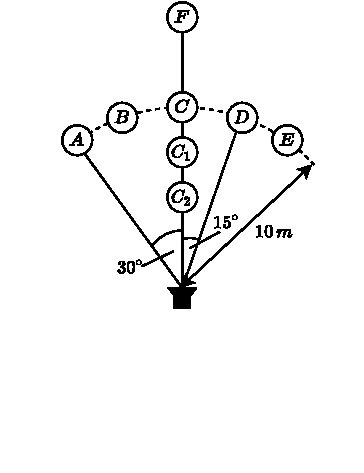
\includegraphics[width=8cm, trim=0mm 22mm 0mm 0mm]{images/6_Measurements/MeasurementSetup.pdf}
    \caption{Measurement Setup Final Tests}
    \label{6_fig:measurement_setup_final}
\end{figure}
\newpage

\subsection{Audio Quality}
To evaluate the audio quality, a rating scale has been developed, based on the Swiss grading system. This is shown in Table \ref{6.1.2_tab:audio_quality}.
\begin{center}
\begin{table}[h!]
\centering
\begin{tabular}{ |m{2.1cm}|m{2.1cm}|m{2.1cm}|m{2.1cm}|m{2.1cm}|m{2.1cm}|}
  \hline 
  1 & 2 & 3 & 4 & 5 & 6\\ 
  \hline
 Completely unrecognizable audio, very distorted and noisy & Hardly anything can be recognized, noise and distortion are dominant & Mostly recognizable audio, distortion and noise clearly audible &  Acceptable hearing experience, speech recognizable without effort & Enjoyable hearing experience, appropriate for daily use &  Outstanding Hi-Fi audio quality, no noise audible \\
 \hline
\end{tabular}
\caption{Audio Quality Grading Scale}
\label{6.1.2_tab:audio_quality}
\end{table}
\end{center}

\subsubsection{Measurements}
\begin{enumerate}
    \item General Audio Quality \\
    To test the general audio quality, music and speech was played. All settings were set to default.
    \begin{center}
     \begin{table}[ht]
    \centering
    \begin{tabular}{ |c|c|c|}
      \hline 
      Test & Average & Variance \\ 
      \hline
     Music quality & 4.2 & 0.46 \\
     \hline
     Speech quality & 4.5 & 0.38 \\
     \hline
    \end{tabular}
    \caption{Audio Quality Score}
    \label{6.1.2_tab:music_audio_quality}
    \end{table}   
    \end{center}
    \item Equalizer \\
    For the second test, the equalizer was changed and the music quality of each preset was tested. The equalizer \textit{Main} was not specifically tested but it is the default equalizer and is mentioned in Table \ref{6.1.2_tab:music_audio_quality_eq} as a comparison.
     \begin{center}
     \begin{table}[ht]
    \centering
    \begin{tabular}{ |c|c|c|}
      \hline 
      Test & Average & Variance \\ 
      \hline
     No equalizer & 4.1 & 0.67 \\
     \hline
     Equalizer: \textit{Lowcut 300Hz} & 4.25 & 0.60 \\
     \hline
     Equalizer: \textit{Sharp} & 4 & 0.66 \\
     \hline
     Equalizer: \textit{Main} & 4.2 & 0.46 \\
     \hline
    \end{tabular}
    \caption{Audio Quality of different Equalizers}
    \label{6.1.2_tab:music_audio_quality_eq}
    \end{table}   
    \end{center}
    \item Modulation Type \\
    At last, the audio quality of the two modulations types \acrshort{am} and \acrshort{mam} were compared. The other settings were again set to default.
    \begin{center}
     \begin{table}[ht]
    \centering
    \begin{tabular}{ |c|c|c|}
      \hline 
      Test & Average & Variance \\ 
      \hline
     \acrshort{am} & 3.9 & 0.40 \\
     \hline
     \acrshort{mam} & 4.4 & 0.34 \\
     \hline
    \end{tabular}
    \caption{Audio Quality of different Modulation Types}
    \label{6.1.2_tab:music_audio_quality_mod}
    \end{table}   
    \end{center}
\end{enumerate}
A more detailed overview of the quality measurements can be seen in Figure \ref{6_fig:box_plot_quality}.
\begin{figure}[h!]
    \centering
    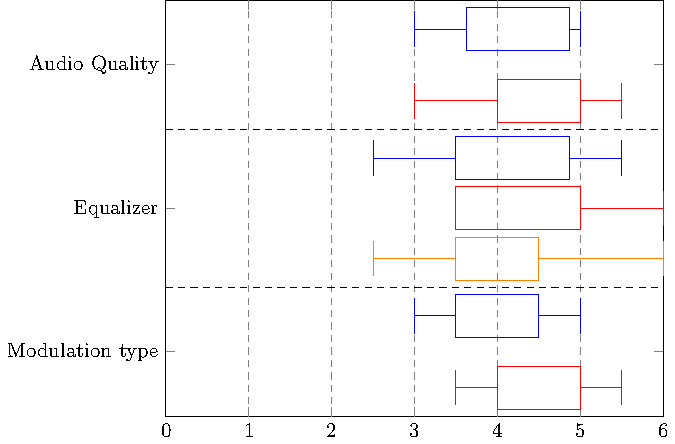
\includegraphics[width=0.7\textwidth]{images/6_Measurements/BoxPlotQuality.pdf}
    \caption{Audio Quality Box-Plot}
    \label{6_fig:box_plot_quality}
\end{figure}

\subsubsection{Evaluation}
The general audio quality test turned out well, as both music and speech were rated on average better than an acceptable hearing experience. Especially the audio quality of speech surprised us and showed that this could be an important use case. In the equalizer test all results turned out to be about the same and statistically show no significant difference between them. We think with more time and more testing better and more impressive equalizer settings can be found and these results can be improved on. 
The modulation type test painted a strong picture that \acrshort{mam} modulation is the way to go. 
Overall, we are very pleased with these results and think a real alternative to conventional loudspeakers can be created with further improvements. 
\newpage

\subsection{Audio Volume}
To evaluate the beam steering capability and overall directivity, a grading system was developed. This is shown in Table \ref{6.1.3_tab:audio_volume}.

\begin{center}
\begin{table}[h!]
\centering
\begin{tabular}{ |m{2.2cm}|m{2.2cm}|m{2.2cm}|m{2.2cm}|m{2.2cm}|}
  \hline 
  -4 & -3 & -2 & -1 & 0\\ 
  \hline
Nearly nothing audible, not noticeable volume level &	Noticeable if background is quiet (no one is talking) &	Strongly noticeable volume level, even with background noise (speech) &	Clearly audible volume level & Very present volume level, strongly dominates background noise
\\
 \hline
\end{tabular}
\caption{Audio Volume Grading Scale}
\label{6.1.3_tab:audio_volume}
\end{table}
\end{center}

\subsubsection{Measurements}
Due to the absolute value of the volume being very objective, the results of each individual test was normalized to be between 1, very loud, and zero, nothing audible. This means that the following list of test results says nothing about the absolute value of the Audio-Beamformer.
\begin{enumerate}
    \item Directivity \\
    To test the directivity, the test person had to rate the volume at every point (A, B, C, D and E). Once with no window applied and once with the Dolph-Chebyshev window, which should, in theory, generate a more directive beam.
    \begin{center}
     \begin{table}[h!]
    \centering
    \begin{tabular}{ |c|c|c|c|c|c|c}
      \hline 
      Test & A & B & C & D & E \\ 
      \hline
     No window & 0.34 & 0.57 & 1 & 0.66 & 0.43 \\
     \hline
     Dolph-Chebyshev & 0.32 & 0.5 & 1 & 0.54 & 0.34 \\
     \hline
    \end{tabular}
    \caption{Audio Directivity}
    \label{6.1.2_tab:music_audio_volume_directivity}
    \end{table}   
    \end{center}
    \item Beam Steering \\
    To test the beam steering, two different tests were carried out.
    \subitem Point C\\
    In the first test, the test person stood on Point C and the beam was steered to an angle of 0, 15 or 30 degrees. This was testes with no window and the Dolph-Chebyshev window.
    \begin{center}
     \begin{table}[h!]
    \centering
    \begin{tabular}{ |c|c|c|c|}
      \hline 
      Test & $0^\circ$ & $15^\circ$ & $30^\circ$ \\ 
      \hline
     No window & 0.98 & 0.8 & 0.83 \\
     \hline
     Dolph-Chebyshev & 1 & 0.72 & 0.70 \\
     \hline
    \end{tabular}
    \caption{Beam Steering Point C}
    \label{6.1.3_tab:music_audio_volume_steering_c}
    \end{table}   
    \end{center}
     \subitem Point A\\
    For the second test, the test person stood on Point A and the beam was steered to an angle of 0, 15 or 30 degrees. This was testes with no window or the Dolph-Chebyshev window.
    \begin{center}
     \begin{table}[h!]
    \centering
    \begin{tabular}{ |c|c|c|c|}
      \hline 
      Test & $0^\circ$ & $15^\circ$ & $30^\circ$ \\ 
      \hline
     No window & 0.55 & 0.71 & 0.96 \\
     \hline
     Dolph-Chebyshev & 0.38 & 0.51 & 1 \\
     \hline
    \end{tabular}
    \caption{Beam Steering Point A}
    \label{6.1.3_tab:music_audio_volume_steering_A}
    \end{table}   
    \end{center}
\end{enumerate}
\subsubsection{Evaluation}
The directivity test showed that already at around $\pm 30^\circ$ the sound is almost only noticeable if the background is quiet. One can also see that the Dolph-Chebyshev window is, as expected, more directive. From the beam steering tests one saw that, especially with no window it is very difficult to keep the point directly in front of the speaker quiet. This is in our opinion mainly due to the inherit directivity of the loudspeaker. The second test, at point A, shows that the beam steering works as expected.
\newpage

\section{Ultrasound Measurements}\label{6_sec:ultrasonic}
As an addition to the human expertise test, a measurement series was carried out. Because we had no sound chamber at our disposal we had to carry out these measurements outside. But due to the surrounding noise, a measurement in the audible spectrum was impossible so all the measurements where carried out only with the carrier. As a result of this, and the difficulties of sound measurement without am ideal setup, measurement device and location these measurements have to be viewed with a pinch of salt.
\subsection{Directivity}
The directivity of the ultrasound was measured with and without a window at 9 distinct points between $-30^\circ$ and $30^\circ$. The results of these measurements are shown in Figure \ref{6.2.1_fig:Directivity_measurements}.
\begin{center}
    \begin{figure}[h!]
        \centering
        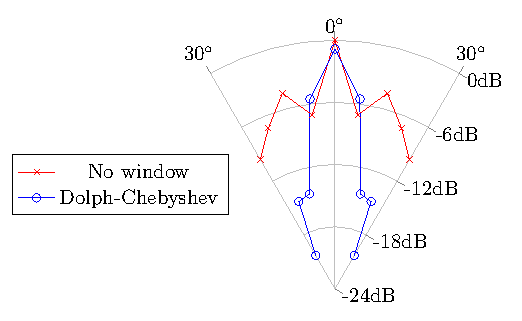
\includegraphics[width=0.5\textwidth]{images/6_Measurements/Polar_PlotDirectivity_Measurement.pdf}
        \caption{Directivity Measurements}
        \label{6.2.1_fig:Directivity_measurements}
    \end{figure}
\end{center}

\subsection{Beam Steering}
To measure the effects of the beam steering, the beam was once directed to $15^\circ$, as seen in Figure \ref{6.2.2_subfig:beamsteering_15}, and once directed to $30^\circ$, as seen in Figure \ref{6.2.2_subfig:beamsteering_30}. The dashed lines in both figures show the on the steered angle mirrored points to give a better feeling of how the beam looks. Due to the inherit directional nature of the loudspeaker, these dashed lines would in practice fall off a lot quicker than shown here. 
\begin{figure}[h!]
    \begin{minipage}{0.49\textwidth}
        \centering
        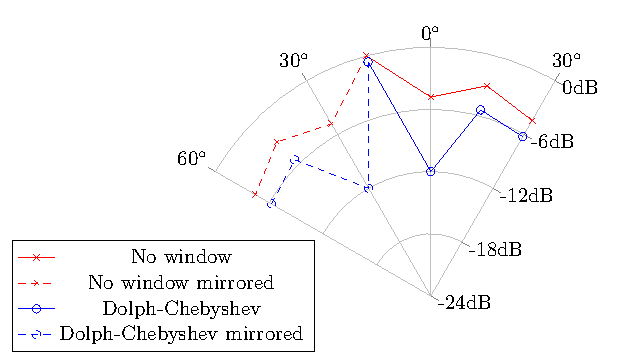
\includegraphics[width=\linewidth]{images/6_Measurements/Polar_PlotSteering_Measurement_15.pdf}
        \caption{Beam steered to 15$^\circ$}
        \label{6.2.2_subfig:beamsteering_15}
    \end{minipage}
    \begin{minipage}{0.49\textwidth}
        \centering
        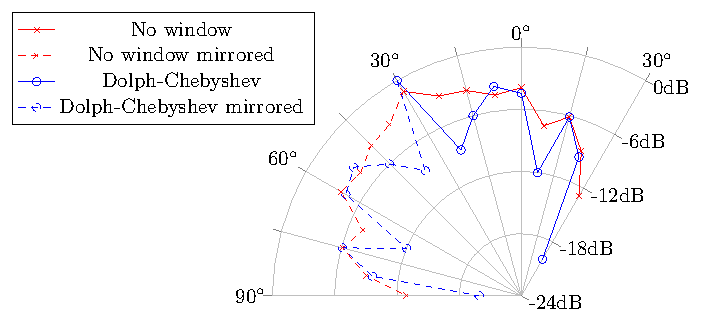
\includegraphics[width=\linewidth]{images/6_Measurements/Polar_PlotSteering_Measurement_30.pdf}
        \caption{Beam steered to 30$^\circ$}
         \label{6.2.2_subfig:beamsteering_30}
    \end{minipage}
\end{figure}

\subsection{Beam Focusing}
The beam focusing was tested on the Points C1 (7.5m), C2 (5m) and F (15m). The results of this are shown in Figure \ref{6_fig:beamforming_measurements}.
\begin{figure}[h!]
    \centering
    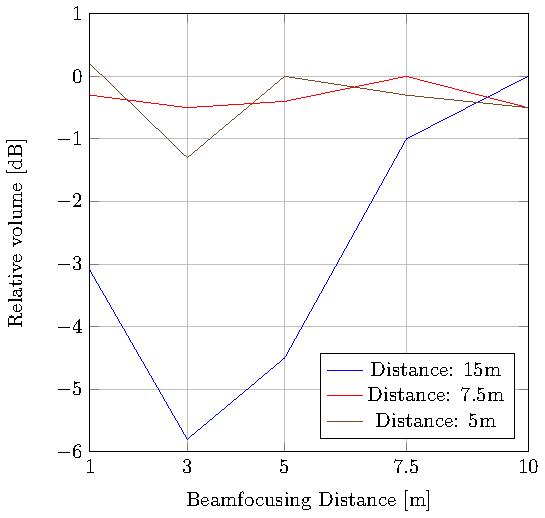
\includegraphics[width=0.4\textwidth]{images/6_Measurements/Beamfocusing.pdf}
    \caption{Beam Focusing Measurements}
    \label{6_fig:beamforming_measurements}
\end{figure}
\subsection{Evaluation}
As already said, due to the imperfect measurement setup these measurements have to be looked at critically. That said, the directivity and beam steering reflect the human expertise tests really well. In comparison to the calculations made in \ref{3_Parametric_array_Sec:Array_signal_processing} the measurements look similar, the main difference is the size of the side lobes, which in our measurements are a lot smaller than calculated. This is most likely due to the directivity of the transducers not being the their assumed sinc function, as shown in Figure \ref{5_fig:directivity_transducer}. 
The beam focusing, on the other hand seems to only work if the distance to the loudspeaker is big enough. To verify further tests have to be made under more ideal conditions. 
\newpage

\section{Transducer Measurements}
To get a better feeling for the transducers and to see how they behave under different circumstances, several measurements where taken. 
\subsection{Frequency Response}\label{6_sec:Frequency_response}
To be able to design more accurate equalizers, the sound pressure level output at each frequency between 22.5\,kHz and 55\,kHz was measured and is shown in Figure \ref{6_Measurement_fig:Transducer_FR}. But again due to no access to a sound chamber these measurements have to be looked at critically.
\begin{figure}[h!]
    \centering
    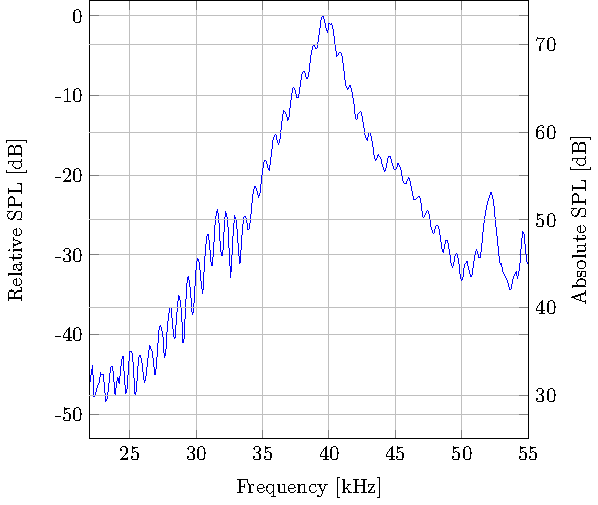
\includegraphics[width=0.5\textwidth]{images/6_Measurements/Transducer_Frequency_Respone.pdf}
    \caption{Frequency Response Transducer}
    \label{6_Measurement_fig:Transducer_FR}
\end{figure}
\subsection{Power Consumption}\label{6_subsec:Power_cons}
The power consumption of each of the 19 transducer lines is very important to access the output power of the loudspeaker. Over a $22 \, \Omega$ resistor in front of the transducer the current could be calculated. The voltage over the transducer and the voltage over the resistor was measured for 4 hours and it turned out that both these values were very constant. The voltage measured over the transducer was $U_T = 9.5 \,$V \acrshort{rms} and the voltage over the resistor $U_R = 1.78 \,$V \acrshort{rms}.
\subsection{Impedance Measurements}\label{6_subsec:impedance_measure}
To get information about the electrical side of the transducers, an impedance measurement was carried out with a series of 20 transducers. It was measured using a vector network analyser.
These measurements can be found in the Audio-Beamformer-software repository (Appendix \ref{Data Archive}).
\newpage
\chapter{Summary \& Conclusion}

\section{Continuing Work}


\begin{itemize}
		\item Testing the device in the field (e.g. installed in a bus). The test results can show the impact of harsh weather conditions, vibrations and other environmental influences.
		\item Beamfocusing improvement
\end{itemize}

\newpage
\section{Reflection}
bla

\section{Personal Reflections}

\subsubsection{Florian Baumgartner}
bla

\subsubsection{Thierry Schwaller}
Made bugs :(

\appendix
\chapter{Appendix}
\clearpage

\section{Declaration of Authorship} \label{Declaration of Authorship}
We hereby certify that the thesis we are submitting is entirely our own original work except where otherwise indicated. We are aware of the University’s regulations concerning plagiarism, including those regulations concerning disciplinary actions that may result from plagiarism. Any use of the works of any other author, in any form, is properly acknowledged at their point of use.

\bigskip
\textbf{Location, Date} \\
Rapperswil, 03. June 2022

\vspace{1.2cm}
\begin{tabular}{@{}p{0.1cm}p{6cm}p{0.6cm}p{6cm}@{}}
& \hrulefill & & \hrulefill\\ \\[-0.7em]
& Florian Baumgartner & & Thierry Schwaller\\
\end{tabular}


\includegraphics[width=4.8cm, align=t, smash=br, hshift=0.9cm, vshift=2.55cm]{appendix/Signature_Florian_Baumgartner.pdf}
%
\includegraphics[width=4.8cm, align=t, smash=br, hshift=8.25cm, vshift=2.77cm]{appendix/Signature_Thierry_Schwaller.pdf}
\newpage

\iffalse

\section{Fleet-Monitor V1.0 Schematics} \label{Fleet-Monitor V1.0 Schematics}
\enlargethispage{2.5cm}
\begin{adjustwidth}{-0.23cm}{0cm} \hfuzz=7.0pt \vfuzz=20.0pt
\makebox[\textwidth]{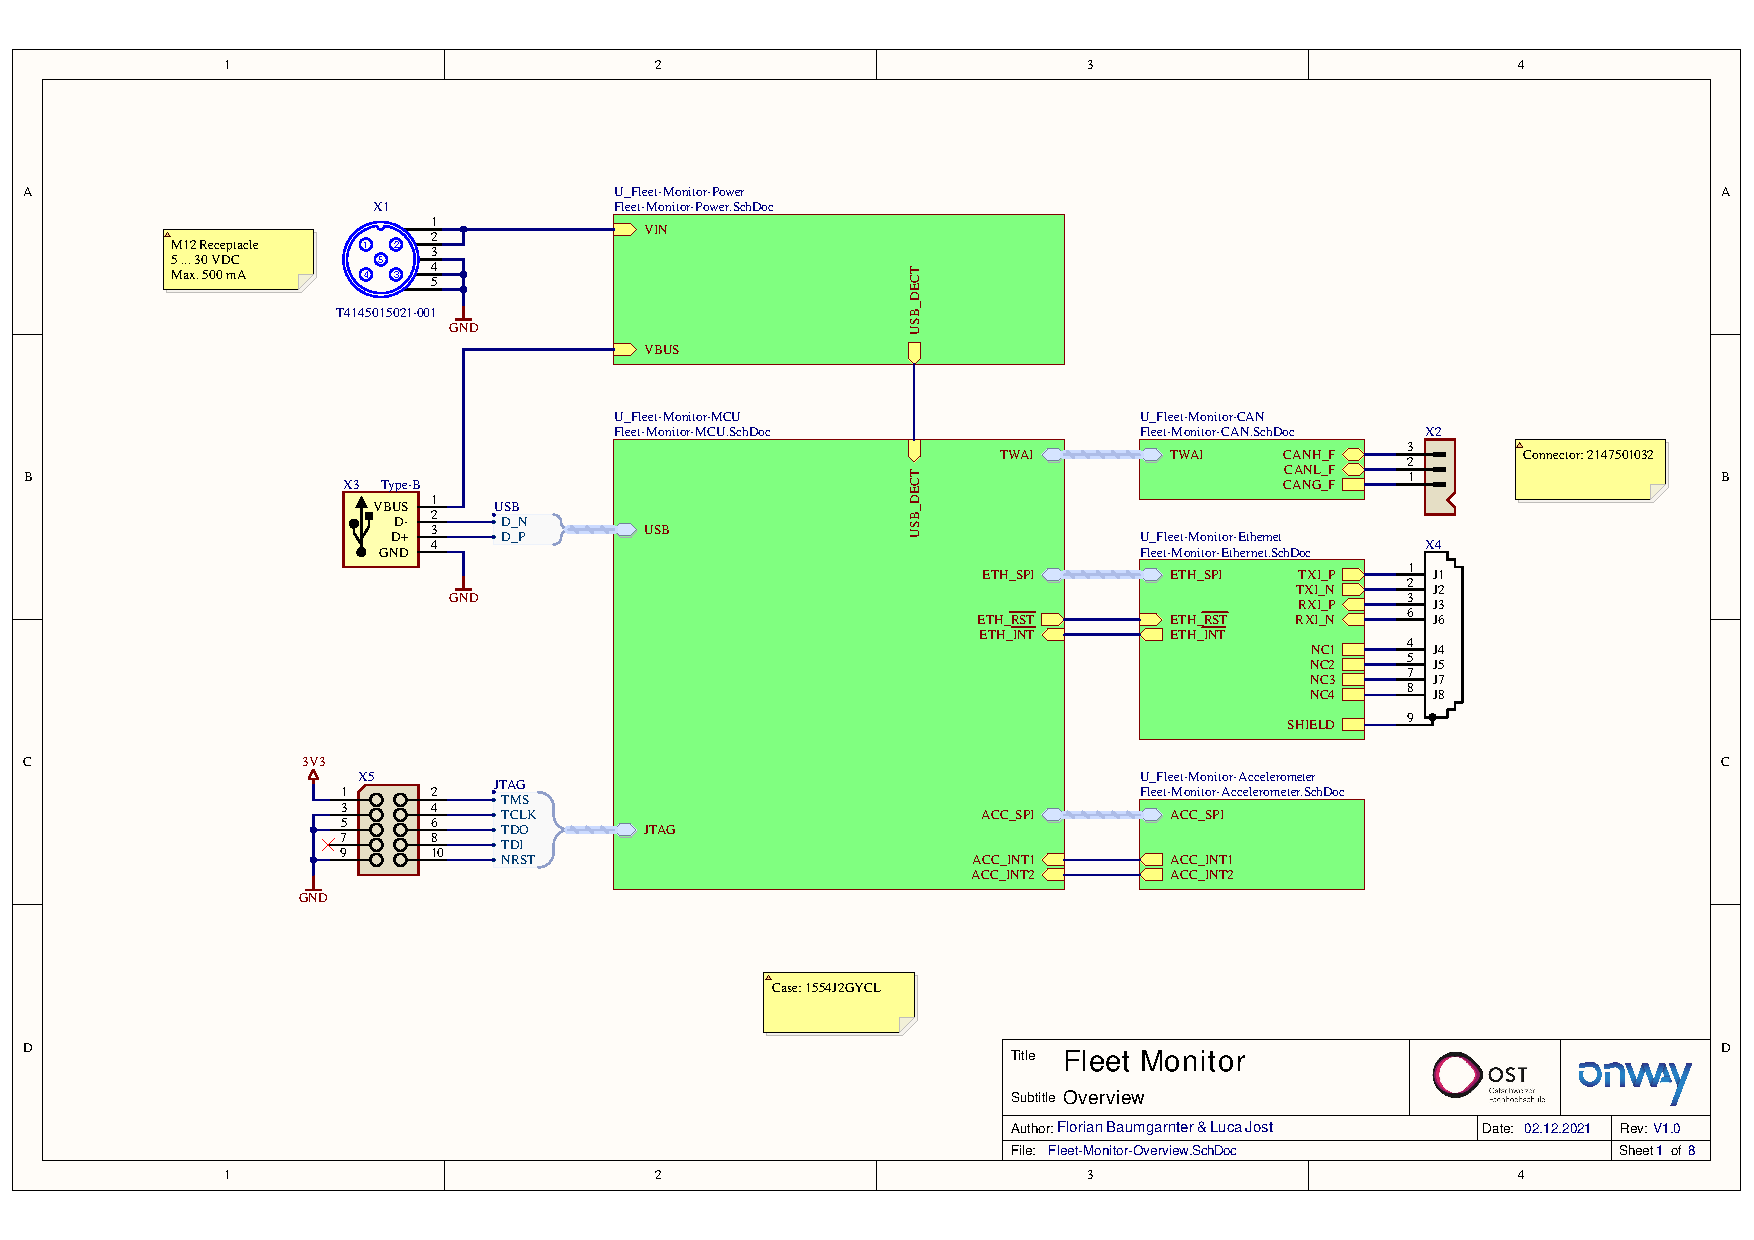
\includegraphics[angle=90, width=17.3cm, page=1]{appendix/Fleet-Monitor Schematics}}
\end{adjustwidth}
\newpage

\begin{adjustwidth}{0.23cm}{0cm} \hfuzz=7.0pt \vfuzz=20.0pt
\makebox[\textwidth]{\includegraphics[angle=90, width=17.3cm, page=2]{appendix/Fleet-Monitor Schematics}}
\end{adjustwidth}
\newpage

\begin{adjustwidth}{-0.23cm}{0cm} \hfuzz=7.0pt \vfuzz=20.0pt
\makebox[\textwidth]{\includegraphics[angle=90, width=17.3cm, page=3]{appendix/Fleet-Monitor Schematics}}
\end{adjustwidth}
\newpage

\begin{adjustwidth}{0.23cm}{0cm} \hfuzz=7.0pt \vfuzz=20.0pt
\makebox[\textwidth]{\includegraphics[angle=90, width=17.3cm, page=4]{appendix/Fleet-Monitor Schematics}}
\end{adjustwidth}
\newpage

\begin{adjustwidth}{-0.23cm}{0cm} \hfuzz=7.0pt \vfuzz=20.0pt
\makebox[\textwidth]{\includegraphics[angle=90, width=17.3cm, page=5]{appendix/Fleet-Monitor Schematics}}
\end{adjustwidth}
\newpage

\begin{adjustwidth}{0.23cm}{0cm} \hfuzz=7.0pt \vfuzz=20.0pt
\makebox[\textwidth]{\includegraphics[angle=90, width=17.3cm, page=6]{appendix/Fleet-Monitor Schematics}}
\end{adjustwidth}
\newpage

\begin{adjustwidth}{-0.23cm}{0cm} \hfuzz=7.0pt \vfuzz=20.0pt
\makebox[\textwidth]{\includegraphics[angle=90, width=17.3cm, page=7]{appendix/Fleet-Monitor Schematics}}
\end{adjustwidth}
\newpage

\begin{adjustwidth}{0.23cm}{0cm} \hfuzz=7.0pt \vfuzz=20.0pt
\makebox[\textwidth]{\includegraphics[angle=90, width=17.3cm, page=8]{appendix/Fleet-Monitor Schematics}}
\end{adjustwidth}
\newpage


\section{Fleet-Monitor V1.0 BOM} \label{Fleet-Monitor V1.0 BOM}
\enlargethispage{1.6cm}
\begin{adjustwidth}{-0.23cm}{0cm} \hfuzz=7.0pt \vfuzz=20.0pt
\makebox[\textwidth]{\includegraphics[angle=90, width=16.5cm]{appendix/Fleet-Monitor_BOM_croped}}
\end{adjustwidth}
\newpage


\section{Fleet-Monitor V1.0 PCB Layout} \label{Fleet-Monitor V1.0 PCB Layout}
\enlargethispage{2.5cm}
\begin{adjustwidth}{0.23cm}{0cm} \hfuzz=7.0pt \vfuzz=20.0pt
\makebox[\textwidth]{\includegraphics[angle=90, width=17.3cm, page=1]{appendix/Fleet-Monitor Layout}}
\end{adjustwidth}
\newpage

\begin{adjustwidth}{-0.23cm}{0cm} \hfuzz=7.0pt \vfuzz=20.0pt
\makebox[\textwidth]{\includegraphics[angle=90, width=17.3cm, page=2]{appendix/Fleet-Monitor Layout}}
\end{adjustwidth}
\newpage

\begin{adjustwidth}{0.23cm}{0cm} \hfuzz=7.0pt \vfuzz=20.0pt
\makebox[\textwidth]{\includegraphics[angle=90, width=17.3cm, page=3]{appendix/Fleet-Monitor Layout}}
\end{adjustwidth}
\newpage

\begin{adjustwidth}{-0.23cm}{0cm} \hfuzz=7.0pt \vfuzz=20.0pt
\makebox[\textwidth]{\includegraphics[angle=90, width=17.3cm, page=4]{appendix/Fleet-Monitor Layout}}
\end{adjustwidth}
\newpage

\begin{adjustwidth}{0.23cm}{0cm} \hfuzz=7.0pt \vfuzz=20.0pt
\makebox[\textwidth]{\includegraphics[angle=90, width=17.3cm, page=5]{appendix/Fleet-Monitor Layout}}
\end{adjustwidth}
\newpage

\begin{adjustwidth}{-0.23cm}{0cm} \hfuzz=7.0pt \vfuzz=20.0pt
\makebox[\textwidth]{\includegraphics[angle=90, width=17.3cm, page=6]{appendix/Fleet-Monitor Layout}}
\end{adjustwidth}
\newpage


\section{Fleet-Monitor V1.0 Mechanical Drawing} \label{Fleet-Monitor V1.0 Mechanical Drawing}
\enlargethispage{2.5cm}
\begin{adjustwidth}{0.23cm}{0cm} \hfuzz=7.0pt \vfuzz=20.0pt
\makebox[\textwidth]{\includegraphics[angle=90, width=17.3cm, page=1]{appendix/Fleet-Monitor Case Drawing}}
\end{adjustwidth}
\newpage

\fi

\section{Datasheet Ultrasonic Transducer} \label{appendix_ma401a6}
\enlargethispage{2.5cm}
\begin{adjustwidth}{-0.23cm}{0cm} \hfuzz=7.0pt \vfuzz=20.0pt
\makebox[\textwidth]{\includegraphics[angle=0, width=17.3cm, page=1]{appendix/MA40A16}}
\end{adjustwidth}
\newpage




\section{Data Archive} \label{Data Archive}
All created files and documents of this project are publicly available on GitHub. An institution called \textbf{SA-OST-2021} (\url{https://github.com/SA-OST-2021}) has been founded which contains repositories for each individual part of the project.
A quick description of the repositories including the associated web link is listed below:

\subsubsection{fleet-monitor-admin} \label{fleet-monitor-admin} \vspace{-0.2cm}
\begin{description}
  \item[Description:] This repository contains all confidential information of the project.\vspace{-0.25cm}
  \item[URL:] \url{https://github.com/SA-OST-2021/fleet-monitor-admin}\vspace{-0.25cm}
  \item[Type:] Private\vspace{-0.25cm}
\end{description}

\subsubsection{fleet-monitor-docs} \vspace{-0.2cm}
\begin{description}
  \item[Description:] This repository contains all additional documentation of the project.\vspace{-0.25cm}
  \item[URL:] \url{https://github.com/SA-OST-2021/fleet-monitor-docs}\vspace{-0.25cm}
  \item[Type:] Public\vspace{-0.25cm}
\end{description}

\subsubsection{fleet-monitor-requirements-specification} \vspace{-0.2cm}
\begin{description}
  \hfuzz=35.0pt
  \item[Description:] This repository contains the Requirements Specification.\vspace{-0.25cm}
  \item[URL:] \url{https://github.com/SA-OST-2021/fleet-monitor-requirements-specification}\vspace{-0.25cm}
  \item[Type:] Public\vspace{-0.25cm}
\end{description}

\subsubsection{fleet-monitor-report} \vspace{-0.2cm}
\begin{description}
  \hfuzz=35.0pt
  \item[Description:] This repository contains this document.\vspace{-0.25cm}
  \item[URL:] \url{https://github.com/SA-OST-2021/fleet-monitor-report}\vspace{-0.25cm}
  \item[Type:] Public\vspace{-0.25cm}
\end{description}

\subsubsection{fleet-monitor-hardware} \vspace{-0.2cm}
\begin{description}
  \item[Description:] This repository contains hardware and mechanical related documents.\vspace{-0.25cm}
  \item[URL:] \url{https://github.com/SA-OST-2021/fleet-monitor-hardware}\vspace{-0.25cm}
  \item[Type:] Public\vspace{-0.25cm}
\end{description}

\subsubsection{fleet-monitor-embedded} \vspace{-0.2cm}
\begin{description}
  \item[Description:] This repository contains firmware source code written in C++.\vspace{-0.25cm}
  \item[URL:] \url{https://github.com/SA-OST-2021/fleet-monitor-embedded}\vspace{-0.25cm}
  \item[Type:] Public\vspace{-0.25cm}
\end{description}

\subsubsection{fleet-monitor-configuration-tool} \vspace{-0.2cm}
\begin{description}
  \item[Description:] This repository contains the filter configuration tool written in Python.\vspace{-0.25cm}
  \item[URL:] \url{https://github.com/SA-OST-2021/fleet-monitor-configuration-tool}\vspace{-0.25cm}
  \item[Type:] Public\vspace{-0.25cm}
\end{description}

\subsubsection{fleet-monitor-network-tool} \vspace{-0.2cm}
\begin{description}
  \item[Description:] This repository contains the network tool (server) written in Python.\vspace{-0.25cm}
  \item[URL:] \url{https://github.com/SA-OST-2021/fleet-monitor-network-tool}\vspace{-0.25cm}
  \item[Type:] Public\vspace{-0.25cm}
\end{description}

\subsubsection{fleet-monitor-visualizer} \vspace{-0.2cm}
\begin{description}
  \item[Description:] This repository contains the graphical data visualizer written in Python.\vspace{-0.25cm}
  \item[URL:] \url{https://github.com/SA-OST-2021/fleet-monitor-visualizer}\vspace{-0.25cm}
  \item[Type:] Public\vspace{-0.25cm}
\end{description}

\subsubsection{fleet-monitor-rasp-image} \vspace{-0.2cm}
\begin{description}
  \item[Description:] This repository contains an image of the Raspberry Pi SD-Card.\vspace{-0.25cm}
  \item[URL:] \url{https://github.com/SA-OST-2021/fleet-monitor-rasp-image}\vspace{-0.25cm}
  \item[Type:] Public\vspace{-0.25cm}
\end{description}

\backmatter

\bibliographystyle{plain}
\typeout{}
\bibliography{./sections/bibliography.bib}

\end{document}